%%% VCU thesis/dissertation template file
\makeatletter
\let\my@xfloat\@xfloat
\makeatother

\documentclass[reqno]{vcuthesis}
\makeatletter
\def\@xfloat#1[#2]{
        \my@xfloat#1[#2]%
        \def\baselinestretch{1}%
        \@normalsize \normalsize
}
\makeatother
%%%%%%%%%%%%
% PACKAGES %
\usepackage{bm,amsmath,subfigure,graphicx,url,algorithm,algorithmicx,algpseudocode,booktabs}
\usepackage{tikz-cd,adjustbox,amsfonts,mathtools,tabularx,capt-of,longtable,comment}
\usepackage[flushleft]{threeparttable}
\usepackage[top=1in,bottom=1in,right=1in,left=1in]{geometry}
\usepackage[backend=bibtex]{biblatex}
\usepackage[titletoc]{appendix}
\usepackage{pgfplots}
\pgfplotsset{compat=1.12}
\usepackage[linktocpage=true]{hyperref}
\usetikzlibrary{shapes.geometric,arrows,automata,positioning}
\usepackage{chngcntr}
\usepackage[final]{pdfpages}
\usepackage[explicit]{titlesec}

\newcommand{\iitem}{\item[-]}
\newcommand{\set}[1]{{\left\{#1\right\}}} 
\newcommand{\norm}[1]{{||#1||}} 
\newcommand{\st}{{\,|\,}} 
\newcommand{\reals}{{\mathbb{R}}}
\newcommand{\ints}{{\mathbb Z}}
\newcommand{\spa}[1]{\mathcal{#1}}
\newcommand\tab[1][1cm]{\hspace*{#1}}
\newcommand{\Rho}{\mathrm{P}}

%%%%%%%%%%%
\overfullrule=5pt
% BIBLIOGRAPHY %
\bibliography{references}
\renewcommand{\type}{Dissertation}
\renewcommand{\thetable}{\arabic{table}}
\newcommand{\comments}[1]{}
%%%%%%%%%%%

% EQUATIONS %
\numberwithin{equation}{chapter}
%%%%%%%%%%%

% DOCUMENT  %
\begin{document}
\counterwithin{figure}{chapter}
\counterwithin{algorithm}{chapter}
\counterwithin{table}{chapter}

\pagenumbering{roman}

\makeatletter
\newcommand\pagenumberingnoreset[1]{\gdef\thepage{\csname @#1\endcsname\c@page}}
\makeatother

\tikzstyle{decision} = [diamond, draw, text centered, inner sep=3pt]
\tikzstyle{block} = [rectangle, draw, fill=gray!20,text width=5em, text centered, rounded corners, minimum height=4em]
\tikzstyle{arrow} = [thick,->,>=stealth]

%%%%%%%%%%%
\newcommand{\thesisordissertation}{Dissertation}
\newcommand{\thesistitle}{\uppercase\expandafter{} Novel Support Vector Machines for Diverse Learning Paradigms}
\newcommand{\authorsname}{Gabriella Angela Melki}
\newcommand{\thesismonth}{August}
\newcommand{\graduatingyear}{2018}
\newcommand{\degree}{Doctor of Philosophy}
\newcommand{\pastdegreeone}{Ph.D. Candidate}
\newcommand{\pastdegreetwo}{MSc. Computer Science, Virginia Commonwealth University, 2016} % 897 in .cls
\newcommand{\committeechair}{Alberto Cano}
\newcommand{\committeechairtwo}{Sebastian Ventura}
\newcommand{\major}{Computer Science}
\newcommand{\school}{Virginia Commonwealth University}
\newcommand{\chairposition}{Assistant Professor}
\newcommand{\chairpositiontwo}{Professor}
\newcommand{\majortwo}{Computer Science \& Numerical Analysis}
\newcommand{\schooltwo}{University of C\'{o}rdoba}

\vspace*{10em}
\begin{center}
\thispagestyle{empty}
\copyright Gabriella Angela Melki, April {\graduatingyear}\\
All Rights Reserved.
\end{center}
\vspace*{\fill}
\maketitlepage

\setlength{\headheight}{12pt}

% ABSTRACT  %

\theabstract{\label{sec:abstractlabel}
This thesis proposes novel support vector machines for two non-traditional learning paradigms, \textit{Multi-Target} Regression and \textit{Multiple-Instance} classification. 

Three multi-target support vector regression (SVR) models are first presented. The first involves building independent, single-target SVR models for each target. The second builds an ensemble of random chains using the first single-target method as a base model. The third calculates the targets' correlations and forms a maximum correlation chain, which is used to build a single chained SVR model, improving the model's prediction performance, while reducing computational complexity.

\sloppypar{Under the multi-instance paradigm, this proposal introduces a novel support vector machine (SVM) multiple-instance formulation, and presents an algorithm with a bag-representative selector that trains the SVM based on bag-level information, named MIRSVM. The contribution is able to identify instances that highly impact classification, i.e. bag-representatives, for both positive and negative bags, while finding the optimal class separation hyperplane. Unlike other multi-instance SVM methods, this approach eliminates possible class imbalance issues by allowing both positive and negative bags to have at most one representative, which constitute as the most contributing instances to the model.}

Rigorous experimental studies and statistical analyses over various metrics and datasets were conducted in order to comprehensively compare the proposed solutions against modern, widely-used methods from both paradigms. The experimental study and analysis confirms that the proposals achieve better performances and more scalable solutions than the methods compared, making them competitive in their respected fields.
}\\

\tableofcontents
\listofalgorithmsvcu
\listoftables
\listoffigures
\clearpage

\pagenumberingnoreset{arabic}

\chapter{Introduction \label{chap:chapintro}}
In traditional classification and regression problems, learning algorithms attempt to correctly predict unknown samples by finding patterns between training samples and their outputs. Identifying these patterns is a non-trivial task due to many factors such as the high dimensionality of the data, as well as the dataset size. 

% first we can talk about volume of data
Over the past decade, dataset sizes have grown disproportionately to the speed of processors and memory capacity, limiting machine learning methods to computational time. Many real-world applications, such as human activity recognition, operations research, and video/signal processing, require algorithms that are scalable and accurate, while being able to provide insightful information in a timely fashion.

% then we introduce the notion of various types of data (mi and mt)
More recently, these traditional methods have been extended to accommodate various types of data paradigms. Examples include \textit{Multiple Target} (MT) learning  and \textit{Multiple Instance} (MI) learning. These emerging paradigms require algorithms to be robust and accommodate non-traditional data representations.

% introduce MT-Regression Problems
Multi-target learning is a challenging task that consists of creating predictive models for problems with multiple outputs. Specifically, MT learning is an approach to transfer learning that improves generalization by using domain information present in training data of multiple related targets as an inductive bias. This is done by learning in parallel, and what is learned for each target can be used to help other targets be learned better~\cite{Baxter1997,Caruana1997,thrun1996learning}. MT learning includes \textit{multi-target regression} (MTR), which addresses the prediction of continuous targets, \textit{multi-label classification}~\cite{Zhang20141819} which focuses on binary targets, and \textit{multi-dimensional classification} which describes the prediction of discrete targets~\cite{Borchani2015}. 

Multi-target prediction has the capacity to generate models representing a wide variety of real-world applications, ranging from natural language processing~\cite{Jeong2009} to bioinformatics~\cite{Lui2010}. A characteristic of the MT datasets used in these applications is that they are generated by a single system, indicating that the nature of the outputs captured has some structure. Even though modeling the multi-variate nature and possible complex relationships between the target variables is challenging, they are more accurately represented by a multi-target model~\cite{Caruana1997,Evgeniou2005}.

Several methods have been proposed for solving such multi-target tasks and can be categorized into two groups. The first being \textit{problem transformation} methods in which the multi-target problem is transformed into multiple single-target (ST) problems, each solved separately using standard classification and regression algorithms. The second being \textit{algorithm adaptation} methods which adapt existing traditional algorithms to predict all the target variables simultaneously~\cite{Borchani2015}. Using \textit{problem transformation} algorithms for a domain of \textit{t} target variables, \textit{t} predictive models must be constructed, each predicting a single-target variable. Prediction for an unseen sample would be obtained by running each of the \textit{t} single-target models and concatenating their results. Conversely, when using \textit{algorithm adaptation} algorithms for the same domain of \textit{t} target variables, a single model would need to be constructed which would output all \textit{t} predictions.

It is known that \textit{algorithm adaptation} methods outperform \textit{problem transformation} methods. The most valuable advantage of using multi-target techniques is that, not only are the relationships between the sample variables and the targets exploited, but the relationships between the targets amongst themselves are as well~\cite{Baxter1997,Caruana1997}. Single-target techniques, on the other hand, eliminate any possibility of learning from the possible relationships between the target variables because a single, independent model is trained for each target separately. Another advantage of MT techniques is model interpretability~\cite{BenDavic2003}. A single multi-target model is highly more interpretable than a series of single-target models. Not only is a single MT model more interpretable, but it could also be considerably more computationally efficient to train, rather than training multiple single-target models individually~\cite{evgeniou2004regularized}. 

Multi-instance learning (MIL) is a generalization of \textit{supervised learning} that has been recently been gaining interest because of its applicability to many real-world problems such as image classification and annotation \cite{Herman2008}, human action recognition \cite{Yi2016}, and drug activity prediction \cite{Dietterich1997}. The difference between MIL and traditional learning is the nature of the data. In the multi-instance setting, a sample is considered a \textit{bag} that contains multiple \textit{instances} and is associated with a single label. The individual instance labels within a bag are unknown and bag labels are assigned based on a multi-instance assumption, or hypothesis. Introduced by Dietterich et. al.~\cite{Dietterich1997}, the standard MI assumption states that a bag is labeled positive if and only if it contains at least one positive instance. Other hypotheses and frameworks have been proposed by Foulds and Frank~\cite{Foulds2010} to encompass a wider range of applications with MI data, but for the scope of this thesis, we will focus on the standard MI assumption.

One of the major complexities associated with MIL is the ambiguity of the relationship between a bag label and the instances within the bag. This stems from the standard MI assumption, where the underlying distribution among instances within positive bags is unknown. There have been different attempts to overcome this complexity, such as ``flattening" the MIL datasets, meaning instances contained in positive bags each adopt a positive label, allowing the use of classical supervised learning techniques~\cite{Ray2005}. This approach assumes that positive bags contain a significant number of positive instances, which may not be the case, causing the classifier to mislabel negative instances within the bag, decreasing the power of the MI model. To overcome this issue, a different MIL approach was proposed, where subsets of instances are selected from positive bags for classifier training~\cite{Maron1998}. One drawback of this type of method is that the resulting training datasets become imbalanced towards positive instances. Model performance further deteriorates when more instances are selected as subsets than needed~\cite{Carbonneau2016}. 

Our MTR and MIL proposals aim to deal with these drawbacks that exist in both paradigms using support vector machines. Support vector machines (SVM), proposed by Cortes and Vapnik~\cite{Cortes1995}, represent popular linear and non-linear (kernelized) learning algorithms based on the idea of a large-margin classifier. They have been shown to improve generalization performance for binary classification problems. SVMs are similar to other machine learning techniques, but literature shows that they usually outperform them in terms of scalability, computational efficiency, and robustness against outliers. They are known for creating sparse and non-linear classifiers, making them suitable for handling large datasets. A traditional approach for training SVMs is the \textit{Sequential Minimal Optimization} (SMO) algorithm~\cite{Platt1998}, a method for solving the L1-SVM's Quadratic Programming (QP) task. 

In this thesis, various approaches are devised for solving machine learning problems for various types of learning paradigms using traditional support vector machine solvers. Specifically, novel algorithms are proposed for solving multi-target regression (a subset of multi-target learning) and multi-instance classification problems. 

\section{Contributions of the Proposal \label{sec:introcontribute} }
% multi-target regression
The current leading MT models are based on ensembles of regressor chains, where random, differently ordered chains of the target variables are created and used to build separate regression models, using the previous target predictions in the chain. The challenges of building MT models stem from trying to capture and exploit possible correlations among the target variables during training, at the expense of increasing the computational complexity of model training. One of the contributions of this proposal aims to investigate the performance changes when building a regression model using two distinct \textit{algorithm adaptation} chaining methods versus building independent single-target models for each target variable using a novel framework. Specifically, this MTR contribution includes:
\begin{itemize}
\iitem Evaluating the performance of a Support Vector Regressor (SVR) as a multi-target to single-target \textit{problem transformation} method to determine whether it outperforms current popular ST algorithms. Its performance is analyzed as a base-line model for MT chaining methods due to the fact that ST methods do not account for any correlation among the target variables.
\newpage
\iitem Building an MT ensemble of randomly chained SVR models (SVRRC), an \textit{algorithm adaptation} approach, inspired by the chaining classification method, Ensemble of Random Chains Corrected (ERCC) {\cite{Spyromitros2014}}, to investigate the effects and advantages of exploiting correlations among target variables during model training, in the context of regression problems. The main issues to be investigated with this approach are the \textit{randomness} of the created chains because they might not capture of correlations between the targets, as well as the time taken to build all the regressors in the ensemble.

\iitem Proposing an MT \textit{algorithm adaptation} model of SVRs that builds a unique chain, capturing the maximum correlation among target outputs, named SVR Correlation Chains (SVRCC). The advantages of using this approach include exploiting the correlations among the targets which leads to an improvement in model prediction performance, and a reduction in computational complexity because a single SVR-chain model is trained, rather than building an ensemble of 10 base regressors.
\end{itemize}

To address the limitations presented by MIL algorithms, this thesis proposes a novel SVM formulation with a bag-representative selector, called Multiple-Instance Representative Support Vector Machine (MIRSVM). The algorithm does not assume any distribution of the instances and is not affected by the number of instances within a bag, making it applicable to a variety of contexts. The key contributions of this work include:
\begin{itemize}
\iitem Reformulating the traditional primal L$1$-SVM problem to optimize over bags, rather than instances, ensuring all the information contained within each bag is utilized during training, while defining bag representative selector criteria.

\iitem Deriving the dual multi-instance SVM problem, with the Karush-Kuhn-Tucker necessary and sufficient conditions for optimality. The dual is maximized with respect to the Lagrange multipliers and provides insightful information about the resulting sparse model. The dual formulation is kernelized with a Gaussian radial basis function, which calculates the distances between bag representatives.

\iitem Devising a unique bag-representative selection method that makes no presumptions about the underlying distributions of the instances within each bag, while maintaining the default MI assumption. This approach eliminates the issue of class imbalance caused by techniques such as flattening or subsetting positive instances from each bag. The key feature of MIRSVM is its ability to identify instances (support vectors) within positive and negative bags that highly impact the model.
\end{itemize}

\chapter{Background}
Support vector machines represent a popular set of learning techniques that have been introduced under Vapnik-Chervonenkis theory of \textit{structured risk minimization} (SRM)~\cite{boser1992training,Cortes1995,Kecman2001,Schoelkopf2002,Shalev2014}. SRM is an inductive principle for the purpose of model selection. It minimizes the expected probability of error, resulting in a generalized model, without making assumptions about the data distribution~\cite{Shalev2014,vapnik2015uniform}. This is the basis for developing the maximal margin classifier~\cite{vapnik2015uniform}. Based on the work of Aizerman et. al.~\cite{Aizerman67theoretical}, Boser et. al.~\cite{boser1992training} generalized the linear algorithm to the non-linear case. Then, Cortes and Vapnik~\cite{Cortes1995} proposed the soft margin SVM; a modification that not only allowed maximal margin classifiers to be applied to non-linearly separable data, but also introduced a regularization parameter to prevent overfitting and gauge generalizability. That same year, the algorithm was extended by Vapnik et. al.~\cite{vapnik2013nature} to the regression case.

This chapter presents a theoretical background of support vector machines. First, the SVM paradigm is discussed in the context of classification, introducing the concepts of the linear \textit{Hard Margin} classifier, and the nonlinear \textit{Soft Margin SVM}. Next, the concept of Support Vector Regression (SVR) is introduced. Afterwards, popular methods for solving the SVM problem are presented and their advantages and problems are discussed. 

\section{Support Vector Machine Classification}
Supervised learning is the process of determining a relationship $f(\bm x)$ by using a training dataset $\mathcal{S} = \{(\bm{x}_1,y_1),\ldots,(\bm{x}_i,y_i),\ldots,(\bm{x}_n,y_n)\}$, which contains $n$ inputs of $d$-dimensionality, $\bm x_i \in \reals^d$, and their class labels $y_i$. In the case of binary classification, $y_i \in \set{+1,-1}$, where $+1$ and $-1$ are the two class labels.

\begin{figure}[t!]
\centering
\begin{minipage}[b]{0.45\textwidth}
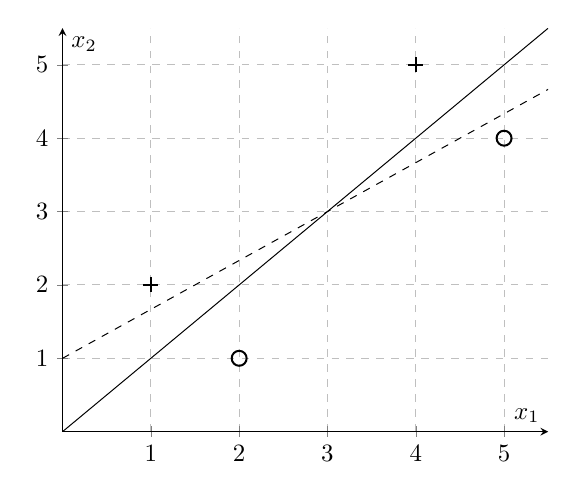
\begin{tikzpicture}[scale=0.9]
\begin{axis}[
    axis lines = center, xlabel = $x_1$, ylabel = $x_2$,
    xtick={0,1,2,3,4,5},ytick={0,1,2,3,4,5},
    ymajorgrids = true,xmajorgrids = true,grid style = dashed,]
%points defined +1
\addplot[only marks, thick, color=black, mark = +, mark size = 3pt]coordinates {(4,5)(1,2)};
%points defined -1
\addplot[only marks, thick, color = black, mark = o, mark size = 3pt]coordinates {(5,4)(2,1)};
%Below the black line is defined
\addplot [dashed,domain = 0:5.5, samples = 10, color = black,]{1/1.5 * x + 1};
%The gray line is defined
\addplot [domain = 0:5.5, samples = 10, color = black,]{x};
\end{axis}
\end{tikzpicture}
\caption{A 2-dimensional example of different possible separating hyperplanes that correctly classify all the toy data points.}
\label{fig:possiblesephyp}
\end{minipage}
\hfill
\begin{minipage}[b]{0.45\textwidth}
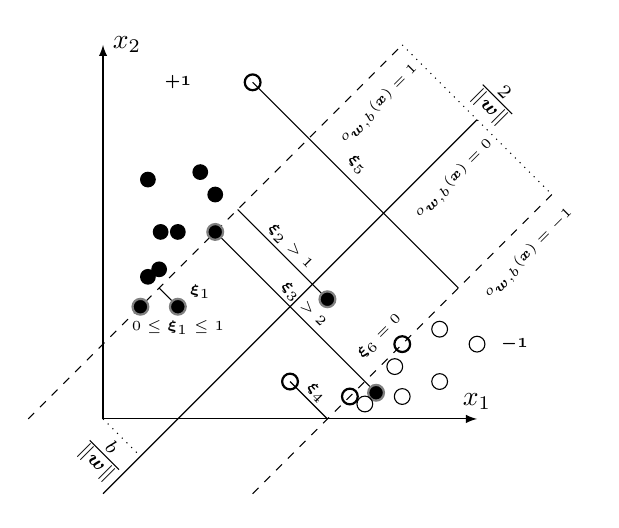
\begin{tikzpicture}[scale = 0.95]
  % Draw axes
  \draw [-latex] (0,0)--(0,5) node  [right]{$x_2$};
  \draw [-latex] (0,0)--(5,0) node  [above]{$x_1$};
  % draw line
  \draw (0,-1) -- (5,4); % y=x-1
  \draw[dashed] (-1,0) -- (4,5); % y=x+1
  \draw[dashed] (2,-1) -- (6,3); % y=x-3
  % \draw labels
  \draw (4.7,3.2) node[rotate=45,font=\tiny] {$o_{\bm w,b}(\bm{x}) = 0$};
  \draw (3.7,4.2) node[rotate=45,font=\tiny] {$o_{\bm w,b}(\bm{x}) = 1$};
  \draw (5.7,2.2) node[rotate=45,font=\tiny] {$o_{\bm w,b}(\bm{x}) = -1$};
  % draw distance
  \draw[dotted] (4,5) -- (6,3);
  \draw (5.25,4.25) node[rotate=-45] {$\frac{2}{\Vert \bm{w} \Vert}$};
  \draw[dotted] (0,0) -- (0.5,-0.5);
  \draw (0,-0.5) node[rotate=-45] {$\frac{b}{\Vert \bm{w} \Vert}$};
  \draw (1,1.5) -- (0.75,1.75);
  \draw (1.3,1.7) node [font=\tiny] {$\bm{\xi}_1$};
  \draw (1,1.225) node [font=\tiny] {$0 \leq \bm{\xi}_1 \leq 1$};
  \draw (3,1.6) -- (1.8,2.8);
  \draw (2.5,2.3) node [rotate=-45, font=\tiny] {$\bm{\xi}_2 > 1$};
  \draw (3.65,0.35) -- (1.5,2.5);
  \draw (2.675,1.525) node [rotate=-45, font=\tiny] {$\bm{\xi}_3 > 2$};
  \draw (2.5,0.5) -- (3,0);
  \draw (2.85,0.35) node [rotate=-45, font=\tiny] {$\bm{\xi}_4$};
  \draw (2,4.5) -- (4.75,1.75);
  \draw (3.4,3.4) node [rotate=-45, font=\tiny] {$\bm{\xi}_5$};
  \draw (5.5,1) node [font=\tiny] {$\bm{-1}$};
  \draw (1,4.5) node [font=\tiny] {$\bm{+1}$};
  \draw (3.7,1.1) node [rotate=45,font=\tiny] {$\bm{\xi}_6 = 0$};
  % draw negative dots
  \draw[thick, draw=gray, fill=black] 	(0.5,1.5) 	circle (3pt);
  \draw[thick, draw=gray, fill=black]   (1.5,2.5)   circle (3pt);
  \draw[thick, draw=gray, fill=black] 	(1,1.5)     circle (3pt);
  \draw[thick, draw=gray, fill=black] 	(3,1.6)     circle (3pt);
  \draw[thick, draw=gray, fill=black] 	(3.65,0.35)     circle (3pt);
  \fill[black] 	(1,2.5)     circle (3pt);
  \fill[black] 	(0.75,2)    circle (3pt);
  \fill[black] 	(0.6,1.9)   circle (3pt);
  \fill[black] 	(0.77, 2.5) circle (3pt);
  \fill[black] 	(1.5,3)     circle (3pt);
  \fill[black] 	(1.3,3.3)   circle (3pt);
  \fill[black] 	(0.6,3.2)   circle (3pt);
  % draw positive dots
  \draw[black,thick] (4,1)     circle (3pt); 
  \draw[black,thick] (3.3,.3)  circle (3pt); 
  \draw[black,thick] (2,4.5)  circle (3pt);
  \draw[black,thick] (2.5,0.5)  circle (3pt);
  \draw[black]     (4.5,1.2) circle (3pt); 
  \draw[black]     (4.5,.5)  circle (3pt); 
  \draw[black]     (3.9,.7)  circle (3pt); 
  \draw[black]     (5,1)     circle (3pt); 
  \draw[black]     (3.5,.2)  circle (3pt); 
  \draw[black]     (4,.3)    circle (3pt); 
\end{tikzpicture}
\caption{An illustration of the soft margin SVM solution on an example $2$-dimensional non-linearly separable dataset.}
\label{fig:nonlinsepdata}
\end{minipage}
\end{figure}

The goal of the soft margin SVM classifier is to find a classification function
\begin{equation}
\centering
f(\bm x) = \textsc{sign } o_{\bm w,b}(\bm x),
\label{eq:classificationfunction}
\end{equation}
where $o_{\bm w,b}(\bm x) = \bm{w}\cdot\bm{x}_i+b$ is a linear decision (output) function representing an affine mapping function $o: \reals^d \rightarrow \reals$ and is parameterized by $\bm w \in \reals^d$, the weight vector, and $b \in \reals$, the bias term. In addition, $\bm w$ and $b$ must satisfy the following,
\begin{equation}
y_i\left( \bm{w} \cdot \bm{x}_i + b\right) \geq 1 - \xi_i, \forall i \in \{1,\ldots,n\},
\label{eqn:softsvmconstraint}
\end{equation}
where $\bm \xi \in \reals^n$ are the non-negative slack variables that allow for some classification error to account for overlapping datasets. The minimal distance between points belonging to opposite classes and the hyperplane is defined as the \textit{margin} and has a width equal to $\frac{2}{||\bm{w}||}$, which is why the $\norm{\bm w}$ must be minimal in order to maximize the margin. 

In the example shown in Figure~\ref{fig:possiblesephyp}, if the training data points are slightly moved, the solid line (with the larger margin) will still correctly classify all the instances, whereas the dotted line (with a much smaller margin, comparatively) will not. This illustrates that the location of the hyperplane has a direct impact on the classifiers generalization capabilities. The hyperplane with the largest margin is called the \textit{optimal separating hyperplane}. Figure~\ref{fig:nonlinsepdata} shows the optimal separating hyperplane for overlapping training data points, where the filled data points are from the $+1$ class and the non-filled data points are from the $-1$ class. The training data points on the separating hyperplane (the circled data points), whose decision function value equals $+1$ or $-1$, are called the \textit{support vectors}. 

The soft margin SVM problem is defined as follows,
\begin{equation}
\label{eq:softsvm}
\begin{aligned}
\min\limits_{(\bm{w},b)} &{\,\,\,\,} \frac{1}{2}||\bm{w}||^2 + C\sum_{i=1}^n \xi_i \\
\text{s.t.} & {\,\,\,\,} y_i\left( \bm{w} \cdot \bm{x}_i + b\right) \geq 1 - \xi_i, {\,\,} \forall i \in \{1,\ldots,n\} \\
 & {\,\,\,\,} \xi_i \geq 0, {\,\,} \forall i \in \{1,\ldots,n\},
\end{aligned}
\end{equation}
where the penalty parameter $C \in \reals$ controls the trade-off between margin maximization and classification error minimization, penalizing large norms and errors. 

Equation~\ref{eq:softsvm} can be rewritten as a regularized loss minimization problem by representing the constraints as the Hinge loss, given by:
\begin{equation}
\centering
L(y_i,\, o_{(w,b)}(\bm{x}_i)) = \max \set{0, 1 - y_i o_{(w,b)}(\bm{x}_i)},
\end{equation}
which penalizes errors satisfying the following: $ y_i o_{(w,b)}(\bm{x}_i) < 1$ and is a crucial element that facilitates the SVM model's sparseness. The soft margin SVM represented as a regularized loss minimization problem becomes:
\begin{equation}
\label{eqn:reghingeloss}
\min\limits_{\bm (\bm{w},b) \in \mathcal{H}_o \times \reals} R {\,\,} = {\,\,} \frac{1}{2}||\bm{w}||^2 + C\sum_{i=1}^n L(y_i,\, o_{(w,b)}(\bm{x}_i)),
\end{equation}
where $\mathcal{H}_o$ is a general Hilbert space. To handle cases when the data are non-linearly separable, while enhancing the classifier's generalization capabilities, a kernel function can be used~\cite{Aizerman67theoretical}, as shown in Equation~\ref{eq:kerneltrick}:
\begin{equation}
\spa{K}\left(\bm{x}_i,\bm{x}_j\right) = \langle \phi\left(\bm{x}_i\right),\,\phi\left(\bm{x}_j\right)\rangle,
\label{eq:kerneltrick}
\end{equation}
where $\phi(\cdot)$ represents a mapping function from the original feature space to a higher dimensional space. The advantage of utilizing kernels is being able to calculate the inner product in the input space rather than in the very high feature dimensional space (including the infinite dimensional ones). The SVM model output, $o$ shown in Equation~\ref{eq:output}, for a given input vector $\bm{x}$ is defined by the kernel as given below:
\begin{equation}
o(\bm x) = \sum_{i = 1}^n \alpha_i \mathcal{K}(\bm x, \bm{x}_i) + b,
\label{eq:output}
\end{equation}
where $\alpha_i \in \reals$ are the coefficients, or weights, of the expansion in feature space, and $b \in \reals$ is the so-called bias term. Note that if a positive definite kernel is used, there is no need for a bias term $b$, but $b$ can nevertheless be used. The two terms, $\bm \alpha$ and $b$, parametrize the SVM model. A model is called \textit{dense} if the absolute value of all its weights are greater than $0$, while a \textit{sparse} model would be one that contains some $\alpha_i = 0$. The level of sparseness may vary, but the sparser the model, the more scalable the applications.

\section{Support Vector Regression}
The support vector machine was applied to the regression case~\cite{Drucker1997,vapnik1997support}, maintaining all the maximal margin algorithmic features. Unlike pattern recognition problems where the desired outputs $y_i$ are discrete, for the regression case they are continuous, real-valued, function outputs. Given training dataset $\mathcal{S} = \set{(\bm x_1,y_1), \ldots, (\bm x_n,y_n) \in \reals^d \times \reals}$, where $y_i \in \reals$ is the continuous output of input $\bm x_i \in \reals^d$, the goal is to learn a function $f(\bm x)$ with at most $\epsilon$ deviation from the true targets $y_i$ for all the training data, while being as flat as possible. This was introduced by Vapnik's linear loss function with $\epsilon$-insensitivity zone, illustrated in Figure~\ref{fig:epsloss} and given by:
\begin{equation}
\label{eq:epsloss}
\centering
|y_i - o_{(w,b)}(\bm{x_i})|_\epsilon = \begin{cases} 
															0 & if |y_i - o_{(w,b)}(\bm{x_i})| \leq \epsilon \\
															|y_i - o_{(w,b)}(\bm{x_i})| - \epsilon & \text{otherwise}.
														\end{cases}
\end{equation}
The loss is equal to 0 if the difference between the predicted and true output values is less than $\epsilon$. Vapnik's $\epsilon$-insensitivity function, shown in Equation~\ref{eq:epsloss}, defines an $\epsilon$-tube, illustrated in Figure~\ref{fig:regressionsvm}. If the predicted value is within the tube, no loss is incurred~\cite{Kecman2001}. Estimating a linear regression hyperplane is achieved by minimizing:
\begin{equation}
\label{eq:regsvmemp}
\min\limits_{(\bm{w},b) \in \mathcal{H}_o \times \reals} R {\,\,} = {\,\,} \frac{1}{2}||\bm{w}||^2 + C\sum_{i=1}^n (|y_i - o_{(w,b)}(\bm{x_i})|_\epsilon).
\end{equation}
Equation~\ref{eq:regsvmemp} is equivalent to the following, where non-negative slack variables are introduced:
\begin{equation}
\label{eq:softsvropt}
\begin{aligned}
\min\limits_{(\bm{w},b,\bm \xi,\bm \xi^*)} & {\,\,\,\,} \frac{1}{2}||\bm{w}||^2 + C\sum_{i=1}^n{\left(\xi_i + \xi^*_i \right)} \\
\text{s.t.} & {\,\,\,\,} y_i - \bm{w} \cdot \bm{x}_i  - b \leq \xi_i + \epsilon, {\,\,} \forall i = \set{1,\ldots,n}\\
				 & {\,\,\,\,} \bm{w} \cdot \bm{x}_i + b - y_i \leq \xi_i^* + \epsilon, {\,\,} \forall i = \set{1,\ldots,n} \\
				 & {\,\,\,\,} \xi_i, \xi^*_i \geq 0, {\,\,} \forall i = \set{1,\ldots,n}.
\end{aligned}
\end{equation}
Note that the constant $C$ influences the trade-off between approximation error and the model generalizability, similar to the classification setting. 
\begin{figure}[t!]
\centering
\begin{minipage}[b]{0.45\textwidth}
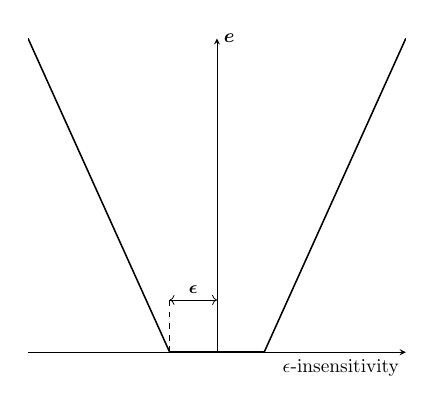
\begin{tikzpicture}[scale=0.7]
\begin{axis}[
	ticks=none,
    axis lines = center, 
    xlabel = $\epsilon\text{-insensitivity}$, 
    xlabel style={below left},
    ylabel = $\bm e$,
    ylabel style={ right}]
% negative epsilon intensity
\addplot [
	thick,
    domain=-4:-1, 
    samples=2, 
    color=black,
]
{- x - 1};
% 0 epsilon intensity
\addplot [
	very thick,
    color=black,
]
coordinates {(-1, 0) (1, 0)};
% positive epsilon intensity
\addplot [
	thick,
    domain=1:4, 
    samples=2, 
    color=black,
]
{ x - 1};
% vertical line indicating where epsilon begines
\addplot[
	color=black,
	style=dashed,
]
coordinates {(-1, 0) (-1, 0.5)};
% epsilon node
\draw[<->] (-1, 0.5) -- (0, 0.5);
\draw (-0.5,0.6) node[font=\small] {$\bm \epsilon$};
\end{axis}
\end{tikzpicture}
\caption{Vapnik's $\epsilon$-insensitivity loss function.}
\label{fig:epsloss}
\end{minipage}
\hfill
\begin{minipage}[b]{0.45\textwidth}
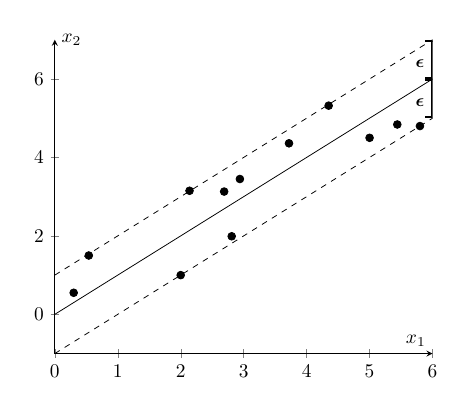
\begin{tikzpicture}[scale = 0.7]
\begin{axis}[
	%ticks = none, 
	axis lines = left, 
	xlabel = $x_1$, 
	xlabel style={at={(1,0)}, above left},
	ylabel = $x_2$,
	ylabel style={at={(0,1)}, right,rotate=-90}
    ]
% main function x
\addplot [
    domain=0:6, 
    samples=2, 
    color=black,
]
{x};
% margin function x + eps
\addplot [
	dashed,
    domain=0:6, 
    samples=2, 
    color=black,
]
{ x+1};
% margin function x - eps
\addplot [
	dashed,
    domain=0:6, 
    samples=2, 
    color=black,
]
{ x - 1};
% epsilon margin
\draw[|-|,very thick] (6,7) -- (6,6);
\draw[|-|,very thick] (6,6) -- (6,5);
\draw (5.8,6.4) node[font=\small] {$\bm \epsilon$};
\draw (5.8,5.4) node[font=\small] {$\bm \epsilon$};
\addplot[color=black,only marks, mark size=2] coordinates {(0.54,1.5) (2,1) (2.14,3.15) (2.94,3.45) (5.8,4.8) (0.30,0.55) (2.69,3.13) (2.81,1.99) (3.72,4.36) (4.35,5.32) (5.44,4.84) (5,4.5) };
\end{axis}
\end{tikzpicture}
\caption{Support vector regression example solution.}
\label{fig:regressionsvm}
\end{minipage}
\end{figure}
The optimization function given in~\ref{eq:softsvropt} can be solved more easily in its dual formulation and is key to extending the SVR to learn from non-linear functions~\cite{Schoelkopf2002}. It is as follows:
\begin{equation}
\label{eq:dualSVR}
\centering
\begin{aligned}
\max\limits_{(\bm \alpha, \bm \alpha^*)} & {\,\,\,\,} -\frac{1}{2} \sum_{i,j = 1}^n (\alpha_i - \alpha^*_i)(\alpha_j - \alpha^*_j)\mathcal{K}(\bm x_i, \bm x_j)  - \epsilon \sum_{i=1}^n (\alpha_i + \alpha^*_i) + \sum_{i=1}^n y_i (\alpha_i - \alpha^*_i) \\
 \text{s.t.} & {\,\,\,\,} \sum_{i=1}^n (\alpha_i - \alpha^*_i) = 0,\, \alpha_i, \alpha^*_i \in [0, C],\, \forall i = \set{1,\,\ldots,n},
 \end{aligned}
\end{equation}
where $\bm \alpha$ and $\bm \alpha^*$ correspond to the SVR dual variables.  

\section{Methods for Solving the SVM Problem}
Although support vector machines represent a major development in machine learning algorithms, in the case of large-scale problems (hundreds of thousands to several millions of samples), the design of SVM training algorithms still has room for improvement. So far, there have been various approaches for tackling large-scale SVM classification problems. 

The first attempts at speeding up the training time and decreasing algorithm memory requirements were aimed at decomposing the underlying SVMs quadratic programming problem. First, Boser et al.~\cite{boser1992training} implemented Vapnik's \textit{chunking} method. \textit{Sequential Minimal Optimization} by Platt~\cite{Platt1998} and its improvement by Keerthie et al.~\cite{keerthi2001improvements} are an alternative approach to decomposing the QP problem, and are implemented in popular, widely used software package LIBSVM~\cite{CC01a}. SMO is an iterative procedure that divides the SVM dual problem into a series of sub-problems, which are solved analytically by finding the optimal $\bm \alpha$ values that satisfy the Karush-Kuhn-Tucker conditions~\cite{Boyd2004}. Although SMO is guaranteed to converge, heuristics are used to choose $\bm \alpha$ values in order to accelerate the convergence rate. This is a critical step because the convergence speed of the SMO algorithm is highly dependent on the dataset size and SVM hyperparameters~\cite{Schoelkopf2002}. 

Some advancements in handling large scale problems are based on a geometric interpretation of SVM problem. Some of these \textit{geometric} SVMs include approaches that use convex hulls~\cite{bennett2000duality} and minimum enclosing balls such as \textit{Core Vector Machines} (CVM)~\cite{tsang2005core}. Tsang et al.~\cite{tsang2007simpler} then improved the scalability of CVMs by introducing \textit{Ball Vector Machines} (BVM) which do not require a QP solver. Other geometric approaches include the novel algorithms introduced by Strack~\cite{strack2013geometric}, known as the \textit{Sphere Support Vector Machine} (SphereSVM) and \textit{Minimal Norm Support Vector Machine} (MNSVM), which utilize the connection between minimal enclosing balls and convex hull problems, while demonstrating a high capability for learning from large datasets. 
The \textit{Non-Negative Iterative Single Data Algorithm} (NNISDA)~\cite{zigic2016} is an efficient approach for solving the SVM problem, shown to be faster than SMO and equal in terms of accuracy~\cite{Kecman2014}. NNISDA is an iterative algorithm that finds a solution to the L2-SVM using coordinate descent, inspired by \textit{Iterative Single Data Algorithm} (ISDA)~\cite{Huang2006} which was originally introduced by Kecman et al.~\cite{Kecman2005}.

Recently, several authors have proposed the use of a standard stochastic gradient descent (SGD) approach for SVMs to optimize large-scale learning problems~\cite{herbrich2016learning,kivinen2002large,Schoelkopf2002,Shalev2014,shalev2011pegasos}. Kivinen et al.\cite{kivinen2004online} and Bousquet and Bottou~\cite{bousquet2008tradeoffs} showed that stochastic algorithms can be both the fastest, and have the best generalization performances. Shalev-Shwartz and Ben-David~\cite{Shalev2014} have also demonstrated that the basic SGD algorithm is very effective when data are sparse, taking less than linear $[O(d)]$ time and space per iteration to optimize a system with $d$ parameters. It can greatly surpass the performance of more sophisticated batch methods on large data sets. The previously mentioned approaches are extended variants of a classic kernel perceptron algorithm~\cite{collobert2004links}. 

Notable representatives of this method of learning include the \textit{Na{\"i}ve Online R Minimization Algorithm} (NORMA) by Kivinen et al.~\cite{kivinen2004online} and the \textit{Primal Estimated Sub-Gradient SOlver for SVM} (PEGASOS) by Shalev-Shwartz et al.~\cite{shalev2011pegasos}. NORMA is an online kernel based algorithm designed to utilize SGD for solving the SVM problem, exploiting the kernel trick in an online setting. It can be regarded as a generalization of the kernel perceptron algorithm with regularization~\cite{kivinen2004online}. PEGASOS solves the primal SVM problem using stochastic sub-gradient descent, implementing both linear and non-linear kernels, and showed that the algorithm does not directly depend on the size of the data, making it suitable for large-scale learning problems. 

A more recent approach, named \textit{OnLine Learning Algorithm} (OLLA)~\cite{kecman2016fast} is a unification, simplification, and expansion of the somewhat similar approaches presented in
~\cite{herbrich2016learning,kivinen2002large,Schoelkopf2002,Shalev2014,shalev2011pegasos} and~\cite{kecman2016ieee,Melki2016,melki2016fast}. This algorithm is unique because it is not only designed to optimize the SVM cost function, but also the cost functions of several other popular nonlinear (kernel) classifiers using SGD in the primal domain. Collobert and Bengio~\cite{collobert2004links} provided justification for not using regularization, and thus OLLA was designed to handle cost functions with and without the regularization term. Comparisons of performances of OLLA with the popular SMO algorithm highlighted the merits of OLLA in terms of speed, as well as accuracy, when the number of samples was increased, making it suitable for large-scale learning. Comparisons using various different classifiers against SMO were also shown~\cite{kecman2016fast}, but for the scope of this proposal the L1-SVM was mentioned.

Although the SGD approaches mentioned above have many merits when it comes to solving large-scale machine learning problems, stochastic procedures also have their disadvantages. One of them stems from the lack of meaningful stopping criteria. The only specified stopping criteria is a user defined input for the number of iterations, which gives rise to the question of what it should be set to. Another disadvantage of kernelized online algorithms is that the training time for each update increases superlinearly with the number of samples. 

\chapter{Multi-Target SVR using Maximum Correlation Chains}
This contribution presents three multi-target support vector regression (SVR) models. The first involves building independent, single-target SVR models for each output variable. The second builds an ensemble of random chains using the first method as a base model, named SVR with Random Chains (SVRRC), inspired by the classification MT method, Ensemble of Random Chains Corrected (ERCC)~\cite{Spyromitros2014}. The third calculates the targets' correlations and forms a maximum correlation chain, which is used to build a single chained model named SVR with Correlation Chaining (SVRCC). The experimental study compares the performance of the three approaches with six other prominent MT regressors. The experimental results are then analyzed using non-parametric statistical tests. The results show that the maximum correlation SVR approach improves the performance of using ensembles of random chains. 

This chapter is organized as follows: Section~\ref{sec:MTRbackground} describes the notation used throughout this chapter and reviews related works on multi-target regression. Section~\ref{sec:MTRproposal} presents the three multi-target support vector regression approaches. Section~\ref{sec:MTRexperiments} presents the experimental study. Section~\ref{sec:MTRresults} discusses the results and the statistical analysis. Finally, Section~\ref{sec:MTRconclusions} shows the main conclusions of this work.

\section{Multi-Target Regression Background}\label{sec:MTRbackground}
This section first defines the notation that will be used throughout this chapter, and then formally describes the multi-target regression problem along with relevant popular algorithms used within this paradigm.

\subsection{Notation}\label{subsec:mtrnotation}
Let $\mathcal{D}$ be a training dataset of $n$ instances. Let $\bm{X} \in \mathcal{D}$ be a matrix consisting of $d$ input variables and $n$ samples, such that $\bm{X} \in \mathbb{R}^{n \times d}$. Let $\bm{Y} \in \mathcal{D}$ be a matrix consisting of $m$ continuous target variables and $n$ samples,  where $\bm{Y} \in \mathbb{R}^{n \times m}$. 

\subsection{Multi-Target Regression}
In the multi-target learning paradigm, the \textit{problem transformation} approach involves training $m$ independent, single-target models for each target output on datasets $\mathcal{D}_j = \set{\bm X, \bm Y_j},\, \forall j \in \{1, \ldots, m\}$, and is considered as a baseline for measuring model performance~\cite{Spyromitros2014}. Many \textit{problem transformation} methods have been proposed for solve multi-target problems, however, the main issue with this type of approach is that the relationships between the targets is lost once independent models are built for each target. Examples of \textit{problem transformation} approaches include Linear Target Combinations for MT Regression~\cite{Tsoumakas2014}, and Multi-Objective Random Forests (MORF) \cite{Kocev2007}. 

The RC, MTS, MTSC, ERC, and ERCC methods are introduced by Spyromitros et. al. in~\cite{Spyromitros2014}. The idea behind these algorithms was to investigate whether advances in multi-label learning can be successfully used in a multi-target regression setting and shed light on modeling target dependencies. These methods involve two stages of learning, the first being building ST models. The second uses the knowledge gained by the first step to predict the target variables while using possible relationships the targets might have with one another. 

The two stages of training in MTS involve firstly, training $m$ independent single-target models, like in ST. In the second step, a second set of $m$ meta models are learned for each target variable, $\bm{Y}_j,\, 1 \leq j \leq m$. These meta models are learned on a transformed dataset, where the input attributes space is expanded by adding the approximated target variables obtained in the first stage, excluding the $j^{th}$ target being predicted.

The ERC method is somewhat similar to the MTS method. In the training of a Regression Chain (RC) model, a random chain, or sequence, of the set of target variables is selected and for each target in the chain, models are built sequentially by using the output of the previous model as input for the next~\cite{Xioufis2016}. If the default, ordered chain is $C = \{\bm Y_1, \bm Y_2, \ldots, \bm Y_m\}$, the first model $h_1 : \bm X \rightarrow \mathbb{R}$ is trained for $\bm Y_1$, as in ST. For the subsequent models $h_{j,j>1}$, the dataset is transformed by sequentially appending the true values of each of the previous targets in the chain to the input vectors. For a new input vector, the target values are unknown. So once the models are trained, the unseen input vector will be appended with the approximated target values, making the models dependent on the approximated values obtained in each step. One of the issues associated with this method is that, if a single random chain is used, the possible relationships between the targets at the head of the chain and the end of the chain are not exploited due to the algorithm's sequential nature. Also, prediction error in the earlier stages of the models will be propagated as the rest of the models are trained, which is why the Ensemble of Regressor Chains was proposed in ~\cite{Spyromitros2014}. Instead of a single chain, $k$ chains are created at random, and the final prediction values are obtained by taking the mean values of the $k$ predicted values for each target. 

In the methods described above, the estimated target variables (meta-variables) are used as input in the second stage of training. In both methods, the models are trained using these meta-variables that become noisy at prediction time, and thus the relationship between the meta-variables and target variable is muddied. Dividing the training set into sets, one for each stage, would not help this situation because both methods would be trained on training sets of decreasing size. Due to these issues, \textit{Spyromitros et. al.} proposed modifications, in \cite{Spyromitros2014}, to both methods that resembles $k$-fold cross-validation (CV) to be able to obtain unbiased estimates of the meta-variables. These methods are called Regression Chains Corrected (RCC) and Multi-Target Stacking Corrected (MTSC). 

The ERCC and MTSC procedures involve repeating the RCC and MTS procedures $k$ times, respectively, with $k$ randomly ordered chains for ERCC, and $k$ different modified training sets for MTSC. The algorithms were tested and compared using Bagging of $100$ regression trees as their base regression algorithm with ERC and ERCC ensemble size of $10$, and $10$-fold cross-validation. The corrected methods exhibited better performance than their original variants, as well as ST models. The ERCC algorithm had the best overall performance, as well as being statistically significantly more accurate of all the methods tested. These methods can be found and used through the open-source Java library, Mulan~\cite{mulan}; to replicate the results found in~\cite{Spyromitros2014}.

\section{Three Novel SVMs for Multi-Target Regression}\label{sec:MTRproposal}
Three novel models have been implemented for the purposes of multi-target regression. The base model is the SVR model, where $m$ single-target soft margin non-linear support vector regressors (NL-SVR) are built for each target variable $\bm Y_j$. 
\begin{figure}[b!]
\begin{minipage}{0.9\textwidth}
\small \centering
\[\begin{tikzcd}[column sep = small, row sep = small]
& & \mathcal{D}_1 :  [\bm X][\bm Y_1]  \arrow[rr]  & & h_1 :  \mathcal{D}_1 \rightarrow \bm{\hat{Y_1}}\\
& & \mathcal{D}_2 :  [\bm X][\bm Y_2]  \arrow[rr] & & h_2 :  \mathcal{D}_2 \rightarrow \bm{\hat{Y_2}} \\        
\mathcal{D} :  [\bm X][\bm Y]  \arrow[uurr, bend left=45] \arrow[urr, bend left] \arrow[drr, bend right]  		& & \vdots \\
& & \mathcal{D}_m :  [\bm X][\bm Y_m] \arrow[rr] & & h_m :  \mathcal{D}_m \rightarrow \bm{\hat{Y}_m}
\end{tikzcd}\]
\end{minipage}
\caption{SVR Flow Diagram. Firstly, the SVR method divides the MT dataset into $m$ ST datasets, $\mathcal{D}_1, \mathcal{D}_2, \ldots, \mathcal{D}_m$. It then independently trains models, $h_1, h_2, \ldots, h_m$, for each ST dataset.}\label{diag:SVR}
\begin{algorithm}[H]
\caption{MT Support Vector Regression (SVR)} \label{alg:SVR} 
\small \centering
\begin{algorithmic}[1]
\renewcommand{\algorithmicrequire}{\textbf{Input:}}
\renewcommand{\algorithmicensure}{\textbf{Output:}}
\Require Training dataset $\mathcal{D}$
\Ensure  ST models $h_j, j = 1,\ldots,m$
\For {$j = 1$ to $m$}
\State $\mathcal{D}_j = \{\bm X, \bm Y_j\}$ \Comment{Get ST data}
\State $h_j : \bm X \rightarrow \mathbb{R}$ \Comment{Build ST model for the $j^{th}$ target}
\EndFor \\
\Return $h_j, j=1,\ldots,m$ 
\end{algorithmic} 
\end{algorithm}
\end{figure}

For NL-SVR, the regularized soft margin loss function given in equation~\eqref{eq:softsvropt} is minimized. This contribution involves solving the dual of this formulation given by \eqref{eq:dualSVR}. Using the dual formulation, the multi-target problem is solved by transforming it into $m$ single-target problems, as shown in Algorithm~\ref{alg:SVR} and Figure~\ref{diag:SVR}. This algorithm will output $m$ single-target models, $h_j,\,\forall j = 1,\ldots,m$, for a given dataset $\mathcal{D}$. It first splits the dataset into $m$ separate ones, $\mathcal{D}_j$, each with a single-target variable $\bm Y_j$, and then builds a distinct SVR model for each of the datasets. 

Building $m$ ST models is a good base-line, but as mentioned previously, it does not capture possible correlations between the target attributes during training. If these correlations are not exploited, this could retract from the model's potential performance. Therefore, creating an ensemble model using a series of random chains was proposed, using the base-line SVR method, named SVR Random Chains (SVRRC). 
\begin{algorithm}[t!]
\centering \small
\caption{Build Chained Model}
\label{alg:buildchainedmodel} 
\begin{algorithmic}[1]
\renewcommand{\algorithmicrequire}{\textbf{Input:}}
\renewcommand{\algorithmicensure}{\textbf{Output:}}
\Require Training dataset $\mathcal{D}$, random chain $\bm C$
\Ensure  A chained model $h_j, j = \{1,\ldots,m\}, c \leq 10$
\State $\mathcal{D}_1 = \set{\bm X, \bm Y_{\bm C_1}}$ \Comment{Initialize first dataset}
\For {$j=1$ to $m$} \Comment{For each target in chain $\bm C$}
\State $h_j : \mathcal{D}_j \rightarrow \mathbb{R}$ \Comment{Train model on appended dataset}
\If {$j < m$}
\State $\mathcal{D}_{j+1} = \set{\mathcal{D}_j, \bm Y_{\bm C_j}}$ \Comment{Append new target in chain to dataset}
\EndIf
\EndFor \\
\Return $h_j, j=1,\ldots,m$ 
\end{algorithmic} 
\end{algorithm}

For SVRRC, ensembles of at most $10$ $m$-sized random chains, $\mathcal{C}$, are built from different and distinct permutations of the target variable indices. When chaining target values, there are two main options: using the predicted value as input for the following target, or using the true value of the target variable as input of the subsequent targets. The main problem with the former approach is that errors are propagated throughout the chained model, therefore SVRCC employs chaining of the true values. 

For each random chain, a new model is trained by predicting the first target variable in the chain. Next, the first target's true value, $\bm Y_j$, is appended to the training set. This chaining process is repeated for all the target indices in the chains, $\{\bm C_1, \ldots, \bm C_c\} \in \mathcal{C}, \, c \leq 10 \,$. This process will be repeated for each random chain generated, returning an ensemble of chained SVRs. Algorithm~\ref{alg:buildchainedmodel} describes the process of building a chained model given chain $\bm C \in \mathcal{C}$, and Algorithm~\ref{alg:SVRRC} shows the steps taken by SVRRC. 

Given this ensemble of chained models, the predicted values for a given unseen instance are calculated by taking the mean of the multiple models generated using different random chains. Since the unseen input has no known target value, the predicted value at each step of the chain $\hat{\bm Y}_j$ is appended to the input at each step of the chain. 
\begin{figure}[t]
\centering \small
\begin{minipage}{\textwidth}
\centering \small
\begin{tikzcd}[column sep = small, row sep = small]
& \mathcal{D} :  [\bm X][\bm Y_1 \bm Y_2 \bm Y_3] \arrow[dl] \arrow[d] \arrow[drr] & & \\
\left[1,2,3\right] \arrow[d] & \left[1,3,2\right] \arrow[d] & \hdots & \left[3,2,1\right] \arrow[d] \\
h_1 :  [\bm X] \rightarrow \bm{\hat{Y_1}} \arrow[d] & h_1 :  [\bm X] \rightarrow \bm{\hat{Y_1}} \arrow[d] & \hdots & h_1 :  [\bm X] \rightarrow \bm{\hat{Y_1}} \arrow[d] \\
h_2 :  [\bm X \bm{Y_1} ] \rightarrow \bm{\hat{Y_2}} \arrow[d] & h_2 :  [\bm X \bm{Y_1} ] \rightarrow \bm{\hat{Y_3}} \arrow[d] & \hdots & h_2 :  [\bm X \bm{Y_3} ] \rightarrow \bm{\hat{Y_2}} \arrow[d] \\
h_3 :  [\bm X \bm{Y_1Y_2} ] \rightarrow \bm{\hat{Y_3}} & h_3 :  [\bm X \bm{Y_1Y_3} ] \rightarrow \bm{\hat{Y_2}} & \hdots & h_3 :  [\bm X \bm{Y_3Y_2} ] \rightarrow \bm{\hat{Y_1}}
\end{tikzcd}
\end{minipage}
\caption{SVRRC Flow Diagram on a dataset with 3 targets. SVRRC first builds the $6$ random chains of the target's indices ($3$ examples are shown). It then constructs a chained model by proceeding recursively over the chain, building a model, and appending the current target to the input space to predict the next target in the chain. } \label{fig:svrrc}
\begin{algorithm}[H]
\caption{MT SVR with Random-Chains (SVRRC)}
\small \centering
\label{alg:SVRRC} 
\begin{algorithmic}[1]
\renewcommand{\algorithmicrequire}{\textbf{Input:}}
\renewcommand{\algorithmicensure}{\textbf{Output:}}
\Require Training dataset $\mathcal{D}$, $c$ random chains $\mathcal{C}$
\Ensure  An ensemble of chained models $h_\mathcal{C}$
\For {\textbf{each }$\bm C \in \mathcal{C}$} \Comment{For each random chain}
\State $h_{\bm C} = $ \text{build chained model}$(\mathcal{D},\bm C)$ \Comment{build a chained model for chain $\bm C$}
\EndFor \\
\Return $h_\mathcal{C}$ 
\end{algorithmic} 
\end{algorithm}
\end{figure}

Due to the computational complexity of building $m!$ distinct chains and training $\left(m!\right) \times m$ models, the number of ensembles and chains are limited to a maximum of $10$. However, if the number of target variables is less than $3$, i.e. $m! \leq 10$, all $m!$ random chains are constructed. 

A disadvantage of building an ensemble of 10 random chains stems from the fact that: when the number of output variables increases, the number of possible chains increases factorially. Therefore, there is no guarantee that the 10 random chains generated will truly reflect the relationships among the target variables. Additionally, building an ensemble of regressors is computationally expensive. Finding a heuristic that allows the identification of a single, most appropriate chain, which fully reflects the output variable interrelations would improve the scalability of training the ensemble. 

The third proposal was designed to remedy this issue. It builds a single chain based on the maximization of the correlations among the target variables. By calculating the correlation of the target variables and imposing it on the order of the chain, this ensures that each appended target provides some additional knowledge on the training of the next. With SVRRC, there is no reasoning behind the generation of these chains, and since the number of random chains generated is limited to $10$, there is no way of ensuring that the $10$ chains fully represent the targets' dependencies. Calculating and using the correlations of the targets would break this uncertainty. Algorithm~\ref{alg:SVRCC} presents the SVR Correlation Chain (SVRCC) method. The computational complexity and hardware constraints (memory size) are negligible during the construction of the targets' correlation matrix, since the correlation matrix would be an $(m \times m)$ matrix, and the likelihood that the number of targets is large enough to cause a memory issue is minimal. 
\begin{figure}[t]
\begin{minipage}{\textwidth}
\centering \small
\begin{tikzcd}
\mathcal{D} :  [\bm X][\bm Y_1 \bm Y_2 \bm Y_3] \arrow{rr}{\textit{generate maximum correlation chain}}[swap]{\frac{\mathbf{E}\left[(Y_i - \mu_i)(Y_j - \mu_j)\right]}{\sqrt{\mathbf{E}\left[(Y_i - \mu_i)(Y_i - \mu_i)\right]\mathbf{E}\left[(Y_j - \mu_j)(Y_j - \mu_j)\right]}}} 
&  \arrow[d, phantom, ""{coordinate, name=Z}]
& \left[1,2,3\right]  \arrow[dll, rounded corners, to path={ -- ([xshift=1ex]\tikztostart.east)
|- ([yshift=-2.5ex]Z) [near end]\tikztonodes
-| ([xshift=-1ex]\tikztotarget.west)
-- (\tikztotarget)}] \\
h_1 :  [\bm X] \rightarrow \bm{\hat{Y_1}} \arrow[r]
& h_2 :  [\bm X \bm{Y_1} ] \rightarrow \bm{\hat{Y_2}} \arrow[r]
& h_3 :  [\bm X \bm{Y_1Y_2} ] \rightarrow \bm{\hat{Y_3}} 
\end{tikzcd}
\end{minipage}
\caption{SVRCC Flow Diagram on a sample dataset with 3 targets. SVRCC first finds the direction of maximum correlation among the targets and uses that order as the only chain. It then constructs the chained model as done in SVRRC. } \label{fig:svrcc}
\begin{algorithm}[H]
\caption{MT SVR with Max-Correlation Chain (SVRCC)} \label{alg:SVRCC} 
\centering \small
\begin{algorithmic}[1]
\renewcommand{\algorithmicrequire}{\textbf{Input:}}
\renewcommand{\algorithmicensure}{\textbf{Output:}}
\State $\bm \Rho = corrcoef(\bm Y)$ \Comment{Find correlation coefficient matrix for target variables}
\State $\bm C = \sum_{i=1}^n \bm \Rho_{ij}, \forall j=1,\ldots,m$ \Comment{Sum row elements of the correlation coefficient matrix}
\State $\bm C = \text{sort}\left(\bm C,\textbf{decreasing}\right)$ \Comment{Sort sums in decreasing order}
\State $h_{\bm C} = $ \text{build chained model}$(\mathcal{D},\bm C)$ \Comment{build a chained model for max correlation chain $\bm C$} \\
\Return $h_{\bm C}$
\end{algorithmic} 
\end{algorithm}
\end{figure}

To calculate the correlation coefficients of the targets, the targets' co-variance matrix, $\bm \Sigma$, is first calculated as shown in Equation~\ref{eq:corr}:
\begin{equation}
\label{eq:corr}
\centering
\bm \Sigma_{ij} = cov(\bm Y_i,\bm Y_j) = \mathbf{E}\left[(\bm Y_i - \mu_i)(\bm Y_j - \mu_j)\right],
\end{equation}
where $\mu_i = \mathbf{E}(\bm Y_i)$, and $\mathbf{E}(\bm Y_i)$ is the expected value of $\bm Y_i$, $\forall i,j \in \{1,\ldots,m\}$. This matrix will show how the targets change together. 

The correlation coefficients matrix, $\bm \Rho$, is then calculated as shown in Equation~\ref{eq:corrcoef}:
\begin{equation}
\label{eq:corrcoef}
\centering
\bm \Rho = corrcoef(\bm Y) = \frac{\bm \Sigma_{ij}}{\sqrt{\bm \Sigma_{ii}\bm \Sigma_{jj}}},\, \forall i,j \in \{1,\ldots,m\}.
\end{equation}
It will describe the linear relationship among the target variables. The coefficients are then sorted in decreasing order, creating the maximum correlation chain. 

\section{Experimental Environment}\label{sec:MTRexperiments}
Although many interesting applications of multi-target regression exist, there are not many publicly available datasets to use. The datasets used in the experimental study were collected from the Mulan website~\cite{mulan}, as well as the UCI Machine Learning Repository~\cite{Lichman:2013}. Information on the $24$ datasets used is summarized in Table~\ref{tab:mtrdatasets}, where the number of samples, attributes (dimensionality), and targets are shown. 
\begin{table}[t!]
\centering \small
\caption{Multi-Target (MT) Regression datasets} \label{tab:mtrdatasets}
\begin{tabular}{lccc}
\noalign{\smallskip}\hline\noalign{\smallskip}
Dataset & Samples $(n)$ & Attributes $(d)$ & Targets $(m)$\\
\noalign{\smallskip}\hline\noalign{\smallskip}
EDM & 145 & 16 & 2\\
Enb & 768 & 8 & 2 \\
Jura & 359 & 11 & 7 \\
Osales & 639 & 413 & 12 \\
Scpf & 1137 & 23 & 3 \\
Slump & 103 & 7 & 3 \\
Solar Flare 1 & 323 & 10 & 3\\
Solar Flare 2 & 1,066 & 10 & 3\\
Water Quality & 1,060 & 16 & 14\\
OES97 & 323 & 263 & 16\\
OES10 & 403 & 298 & 16\\
ATP1d & 201 & 411 & 6\\
ATP7d & 188 & 411 & 6\\
Andro & 49 & 30 & 6 \\
Wisconsin Cancer & 198 & 34 & 2\\
Stock & 950 & 10 & 3\\
California Housing & 20,640 & 7 & 2\\
Puma8NH & 8,192 & 8 & 3\\
Puma32H & 8,192 & 32 & 6\\
Friedman & 500 & 25 & 6\\
Polymer & 41 & 10 & 4\\
M5SPEC & 80 & 700 & 3\\
MP5SPEC & 80 & 700 & 3\\
MP6SPEC & 80 & 700 & 3\\
\noalign{\smallskip}\hline\noalign{\smallskip}
\end{tabular}
\end{table}

Experiments were performed over the RC, ST, MTS, MTSC, ERC, ERCC, and MORF algorithms, which have also been used in the experimental study conducted in~\cite{Spyromitros2014}. These algorithms were chosen because they have shown considerable performance in training multi-target models. The have also made their framework readily available for reproducing their results. All three SVR algorithms are implemented within the general framework of Mulan's MTRegressor\footnote{http://mulan.sourceforge.net}~\cite{mulan}, which was built on top of Weka\footnote{http://www.cs.waikato.ac.nz/ml/weka}~\cite{Hall2009}. LIBSVM's Epsilon-SVR~\cite{CC01a} implementation was used as the base SVR model. The parameters experimented with for the SVR regression task are the penalty parameter $C$, the Gaussian kernel parameter $\gamma$, and the error or tube parameter $\epsilon$ given by Equations~\eqref{eq:paramCmtr} to~\eqref{eq:paramE}, referred to as~\eqref{eq:hyperparammtr}.
\begin{subequations}
\label{eq:hyperparammtr}
\begin{align}
C \in  & \{1, 10, 100\} \label{eq:paramCmtr}\\
\gamma \in  & \{1^{-9}, 1^{-7}, 1^{-5}, 1^{-3}, 1^{-1}, 1, 5, 10\} \label{eq:mtrparamG}\\
\epsilon \in  & \{0.01, 0.1, 0.2\} \label{eq:paramE}
\end{align}
\end{subequations}

To ensure a controlled environment when conducting the performance comparisons, the experimental environment for running the competing algorithms was the same as what was done in~\cite{Spyromitros2014}. This includes the following. The ST base-line model used was Bagging~\cite{Breiman1996} of 100 regression trees~\cite{Wu2015430}. The MTSC and ERCC methods are run using $10$-fold cross-validation, and the ensemble size for the ERC and ERCC methods was set to $10$. The ensemble size of 100 trees was used for MORF, and the rest of its parameters were set as recommended by~\cite{Kocev2013}.

The performance metrics used to analyze our contributions' performances are shown in Equations~\ref{eqn:aCC} to~\ref{eqn:arrmse}. For unseen or test datasets of size $\mathcal N_{test}$, the performances are evaluated by taking the run time (seconds) each algorithm takes to build a classifier, as well as the following metrics, where the upwards arrow $\uparrow$ indicates maximizing the metric and the downwards arrow $\downarrow$ indicates minimizing the metric.

\begin{itemize}
\item The average correlation coefficient (aCC $\uparrow$):
\begin{eqnarray}
\frac{1}{m} \sum_{j = 1}^m \frac{\sum_{l = 1}^{\mathcal N_{test}} (y_j^{(l)} - \bar{y}_j)(\hat{y}_j^{(l)} - \bar{\hat{y}}_j)}{\sqrt{\sum_{l = 1}^{\mathcal N_{test}} (y_j^{(l)} - \bar{y}_j)^2 \sum_{l = 1}^{\mathcal N_{test}} (\hat{y}_j^{(l)} - \bar{\hat{y}}_j)^2}}
\label{eqn:aCC}
\end{eqnarray}

\item The mean squared error (MSE $\downarrow$):
\begin{eqnarray}
\frac{1}{m} \sum_{j = 1}^m \frac{1}{\mathcal N_{test}} \sum_{l = 1}^{\mathcal N_{test}} (y_j^{(l)} - \hat{y}^{(l)}_j)^2
\label{eqn:MSE}
\end{eqnarray}

\item The average root mean squared error (aRMSE $\downarrow$):
\begin{eqnarray}
\frac{1}{m} \sum_{j = 1}^m \sqrt{\frac{\sum_{l = 1}^{\mathcal N_{test}} (y_j^{(l)} - \hat{y}^{(l)}_j)^2}{\mathcal N_{test}}}
\label{eqn:armse}
\end{eqnarray}

\item The average relative root mean squared error (aRRMSE $\downarrow$):
\begin{eqnarray}
\frac{1}{m} \sum_{j = 1}^m \sqrt{\frac{\sum_{l = 1}^{\mathcal N_{test}} (y_j^{(l)} - \hat{y}_j^{(l)})^2}{\sum_{l = 1}^{\mathcal N_{test}} (y_j^{(l)} - \bar{y}_j)^2}}
\label{eqn:arrmse}
\end{eqnarray}
\end{itemize}

The predicted output is represented by $\hat{\textbf{y}}$, the average of the predicted output is $\bar{\hat{\textbf{y}}}$, and the average of the true output target variable is $\bar{\textbf{y}}$. The test dataset is the hold-out set during cross validation. This ensures our model is evaluated on data that it has not been trained on, and thus unbiased towards the training datasets. It also contributes to the generalizability and robustness of the model.

\section{Results \& Statistical Analysis}\label{sec:MTRresults}
Tables~{\ref{tab:mtraccResults}},~{\ref{tab:mseResults}},~{\ref{tab:armseresults}},~{\ref{tab:arrmseresults}}, and~{\ref{tab:timeresults}} show the results of our algorithm implementations compared with those of \textit{RC, MORF, ST, MTS, MTSC, ERC,} and \textit{ERCC}. Each subsection discusses a single metric along with the statistical analysis of the results. The best metric value obtained on each dataset is typeset in bold. Non-parametric statistical tests are then used to validate the experiments results obtained. To determine whether significant differences exist among the performance and results of the algorithms, the Iman-Davenport non-parametric test is run to rank the algorithms over the datasets used, according to the Friedman test. The average ranks are presented in the last row of the results tables. The Bonferroni-Dunn post-hoc test~{\cite{Dunn1961}} is then used to find these differences that occur between the algorithms. Below each result table, a diagram highlighting the critical distance (in gray) between each algorithm is shown. The Wilcoxon, Nemenyi, and Holm~{\cite{Wilcoxon1945}} tests were run for each of the result metrics to compute multiple pairwise comparisons among the algorithms used in the experimental study. Tables~{\ref{tab:statacc}},~{\ref{tab:statmse}},~{\ref{tab:statarmse}},~{\ref{tab:statarrmse}}, and~{\ref{tab:stattime}} show the sum of ranks $R^+$ and $R^-$ of the Wilcoxon rank-sum test, and the $p$-values for the $3$ tests, which show the statistical confidence rather than using a fixed $\alpha$ value.

\subsection{Average Correlation Coefficient}\label{subsec:acc}
\begin{table}[t!]
\centering \small
\caption{Average Correlation Coefficient (aCC) for MT regressors}\label{tab:mtraccResults}
\resizebox{0.95\textwidth}{!}{\begin{tabular}{l@{\extracolsep{\fill}}ccccccccccc}
\noalign{\smallskip}\hline\noalign{\smallskip}
Datasets &MORF &ST &MTS &MTSC &RC &ERC &ERCC &SVR &SVRRC &SVRCC \\
\noalign{\smallskip}\hline\noalign{\smallskip}
Slump &0.6965 &0.7062 &0.7163 &0.6977 &0.6956 &0.6977 &0.7023 &0.7245 &0.7339 &\textbf{0.7457} &  \\
Polymer &0.7305 &0.7336 &0.7371 &0.7228 &0.7015 &0.7029 &0.7222 &0.7634 &0.7857 &\textbf{0.7905} &  \\
Andro &\textbf{0.7349} &0.6454 &0.6793 &0.6581 &0.6915 &0.6806 &0.6653 &0.6880 &0.6951 &0.7056 &  \\
EDM &\textbf{0.6722} &0.6352 &0.6412 &0.6354 &0.6355 &0.6379 &0.6354 &0.6484 &0.6565 &0.6567 &  \\
Solar Flare 1 &0.1083 &0.1258 &0.1034 &0.1193 &\textbf{0.1492} &0.1387 &0.1292 &0.1066 &0.0857 &0.1152 &  \\
Jura &0.7854 &0.7907 &0.7880 &0.7882 &0.7877 &0.7884 &0.7897 &0.7789 &0.7921 &\textbf{0.7983} &  \\
Enb &0.9828 &0.9832 &0.9822 &0.9829 &0.9813 &0.9823 &0.9837 &0.9858 &0.9867 &\textbf{0.9868} &  \\
Solar Flare 2 &0.2357 &0.2295 &0.2375 &0.2343 &0.2302 &0.2351 &\textbf{0.2432} &0.1470 &0.1648 &0.1656 &  \\
Wisconsin Cancer &0.3362 &0.3587 &\textbf{0.3652} &0.3588 &0.3628 &0.3609 &0.3590 &0.3187 &0.3208 &0.3373 &  \\
California Housing &0.7705 &0.7720 &0.7149 &0.7451 &0.7007 &0.7844 &\textbf{0.8065} &0.7847 &0.7949 &0.8007 &  \\
Stock &0.9785 &0.9747 &0.9755 &0.9752 &0.9753 &0.9757 &0.9763 &0.9825 &\textbf{0.9829} &0.9822 &  \\
SCPF &0.5827 &0.5508 &0.5503 &0.5477 &0.5569 &0.5656 &0.5515 &0.5891 &\textbf{0.5975} &0.5946 &  \\
Puma8NH &0.5424 &0.4828 &0.4942 &0.4205 &0.4677 &0.4656 &0.4650 &\textbf{0.6041} &0.5975 &0.6038 &  \\
Friedman &0.1507 &0.1609 &0.1548 &0.1667 &0.1558 &0.1608 &0.1632 &0.1710 &0.1748 &\textbf{0.1752} &  \\
Puma32H &0.3085 &0.2934 &0.2890 &0.2504 &0.2754 &0.2870 &0.2797 &0.3358 &0.3351 &\textbf{0.3385} &  \\
Water Quality &\textbf{0.4303} &0.4063 &0.4019 &0.4051 &0.3992 &0.4052 &0.4147 &0.3545 &0.3828 &0.3857 &  \\
M5SPEC &0.8161 &0.8346 &0.8134 &0.8228 &0.8333 &0.8340 &0.8308 &0.9451 &0.9452 &\textbf{0.9472} &  \\
MP5SPEC &0.8315 &0.8536 &0.8244 &0.8535 &0.8524 &0.8526 &0.8542 &0.9560 &0.9602 &\textbf{0.9633} &  \\
MP6SPEC &0.8317 &0.8531 &0.8231 &0.8531 &0.8507 &0.8515 &0.8541 &0.9444 &0.9500 &\textbf{0.9528} &  \\
ATP7d &0.8260 &0.8408 &0.8422 &\textbf{0.8474} &0.8273 &0.8351 &0.8464 &0.8305 &0.8407 &0.8400 &  \\
OES97 &0.7829 &0.7995 &0.7990 &0.8001 &0.7986 &0.7990 &0.7999 &0.8116 &0.8134 &\textbf{0.8137} &  \\
Osales &0.7186 &0.6912 &0.7104 &0.7076 &0.6357 &0.7136 &\textbf{0.7193} &0.6511 &0.6433 &0.6677 &  \\
ATP1d &0.8961 &0.9066 &0.9051 &0.9075 &0.9048 &0.9081 &0.9071 &0.9092 &\textbf{0.9130} &0.9100 &  \\
OES10 &0.8708 &0.8808 &0.8805 &0.8806 &0.8804 &0.8804 &0.8809 &0.8911 &0.8924 &\textbf{0.8963} &  \\
\noalign{\smallskip}\hline\noalign{\smallskip}
Average &0.6508 &0.6462 &0.6429 &0.6409 &0.6396 &0.6476 &0.6492 &0.6634 &0.6685 &\textbf{0.6739} &  \\
Ranks &6.4167 &5.8958 &6.6042 &6.4792 &7.5208 &5.8958 &4.8542 &4.7917 &3.7083 &\textbf{2.8333} &  \\
\noalign{\smallskip}\hline
\end{tabular}}
\centering \small
\resizebox{0.95\textwidth}{!}{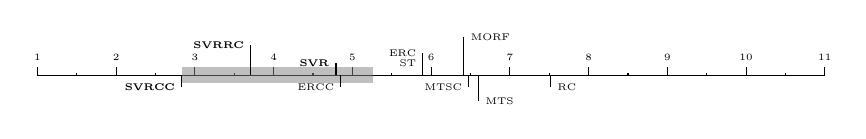
\begin{tikzpicture}
 %axis
 \draw (1,0) -- (11,0);
 \foreach \x in {1,2,3,4,5,6,7,8,9,10,11} {
  \draw (\x, 0) -- ++(0,.1) node [above,scale=0.7] {\tiny \x};
  \ifthenelse{\x < 11}{\draw (\x+.5, 0) -- ++(0,.03);}{}
 }
 % coordinates
 \coordinate (c0) at (2.8333,0);
 \coordinate (c1) at (3.7083,0);
 \coordinate (c2) at (4.7917,0);
 \coordinate (c3) at (4.8542,0);
 \coordinate (c4) at (5.8958,0);
 \coordinate (c5) at (7.5208,0);
 \coordinate (c6) at (6.4792,0);
 \coordinate (c7) at (6.6042,0);
 \coordinate (c8) at (5.8958,0);
 \coordinate (c9) at (6.4167,0);

 % labels
 \node (l0) at (c0) [below left=.025cm and 0cm, align=right, scale=0.7] {\tiny \textbf{SVRCC}};
 \node (l1) at (c1) [above left=.25cm and 0cm, align=right, scale=0.7] {\tiny \textbf{SVRRC}};
 \node (l2) at (c2) [above left=.025cm and 0cm, align=right, scale=0.7] {\tiny \textbf{SVR}};
 \node (l3) at (c3) [below left=.025cm and 0cm, align=left, scale=0.7] {\tiny ERCC};
 \node (l4) at (c4) [above left=.15cm and 0cm, align=right, scale=0.7] {\tiny ERC};
 \node (l5) at (c5) [below right=.025cm and 0cm, align=left, scale=0.7] {\tiny RC};
 \node (l6) at (c6) [below left=.025cm and 0cm, align=right, scale=0.7] {\tiny MTSC};
 \node (l7) at (c7) [below right=.2cm and 0cm, align=left, scale=0.7] {\tiny MTS};
 \node (l8) at (c8) [above left=.025cm and 0cm, align=right, scale=0.7] {\tiny ST};
 \node (l9) at (c9) [above right=.35cm and 0cm, align=right, scale=0.7] {\tiny MORF};

 % CD = 1.4845
 \fill[fill=gray,fill opacity=0.5] (2.8333,-0.1) rectangle (5.2569,0.1);
 
 % connectors
 \foreach \x in {0,...,9} {
  \draw (l\x) -| (c\x);
 };
\end{tikzpicture}}\vspace{-1em}
\captionof{figure}{Bonferroni-Dunn test for aCC}\label{fig:BonfDunnACC}\vspace{-1.5em}
\captionof{table}{Wilcoxon, Nemenyi, and Holm tests for aCC}\label{tab:statacc}
\scriptsize
\resizebox{0.95\textwidth}{!}{\begin{tabular}{lccccc}
\noalign{\smallskip}\hline\noalign{\smallskip}
SVRCC vs. & Wilcoxon $R^{+}$ & Wilcoxon $R^{-}$ & Wilcoxon $p$-value & Nemenyi $p$-value & Holm $p$-value \\ 
\noalign{\smallskip}\hline\noalign{\smallskip}
MORF & 224.0 & 76.0 & $3.4E^{-2}$ & $4.1E^{-5}$& $8.3E^{-3}$ \\
ST & 239.0 & 61.0 & $9.6E^{-3}$ & $4.6E^{-4}$ & $1.3E^{-2}$ \\ 
MTS & 242.0 & 58.0 & $7.2E^{-3}$ & $1.6E^{-5}$ & $6.3E^{-3}$ \\ 
MTSC & 238.0 & 62.0 & $1.1E^{-2}$ & $3.0E^{-5}$ & $7.1E^{-3}$ \\ 
RC & 250.0 & 50.0 & $3.1E^{-3}$ & 0.0000 & $5.6E^{-3}$ \\
ERC & 229.0 & 71.0 & $2.3E^{-2}$ & $4.6E^{-4}$ & $1.0E^{-2}$ \\ 
ERCC & 221.0 & 79.0 & $4.3E^{-2}$ & $2.1E^{-2}$ & $1.7E^{-2}$ \\ 
SVR & 297.0 & 3.00 & $6.0E^{-7}$ & $2.5E^{-2}$ & $2.5E^{-2}$ \\ 
SVRRC & 266.5 & 33.5 & $4.0E^{-4}$ & $3.2E^{-1}$ & $5.0E^{-2}$ \\ 
\noalign{\smallskip}\hline\noalign{\smallskip}
\end{tabular}}
\end{table}
Table~{\ref{tab:mtraccResults}} shows that our proposed methods perform the best on $15$ out of the $24$ datasets. Specifically, the maximum correlation chain method, SVRCC, performs the best on $11$, which is better than the total number of datasets the competing methods performed better at ($9$). The Iman-Davenport statistic, distributed according to the F-distribution with 9 and 207 degrees of freedom is $6.72$, with a $p$-value of $1.9E^{-8}$ which is significantly less than $0.01$, implying a statistical confidence larger than $99\%$. Therefore, we can conclude that there exist statistically significant differences between the aCC results of the algorithms.

Figure~{\ref{fig:BonfDunnACC}} shows the mean rank values of each algorithm along with the critical difference value, $2.4236$, for $\alpha = 0.05$. The algorithms that are to the right of the critical difference rectangle are the ones with significantly different results. Therefore, the $6$ out of $10$ algorithms beyond the critical difference perform significantly worse than our control algorithm, SVRCC. Table~{\ref{tab:statacc}} provides complementary analysis of the results. According to the Wilcoxon test, SVRCC is shown to have significantly better performance over all algorithms with $p$-value $< 0.05$. The Nemenyi and Holm tests show that SVRCC performs significantly better than $6$ out of the $9$ algorithms with $p$-value $\leq 5.6E^{-3}$ and $\leq 1.7E^{-2}$, respectively. The exact confidence for algorithm SVRCC against all others is $0.95$.

\begin{table}[b!]
\centering \small
\caption{Mean Square Error (MSE) for MT regressors}\label{tab:mseResults}
\resizebox{0.95\textwidth}{!}{\begin{tabular}{l@{\extracolsep{\fill}}ccccccccccc}
\noalign{\smallskip}\hline\noalign{\smallskip}
Datasets &MORF &ST &MTS &MTSC &RC &ERC &ERCC &SVR &SVRRC &SVRCC \\
\noalign{\smallskip}\hline\noalign{\smallskip}
Slump &1.4388 &1.4161 &1.3667 &1.4414 &1.4602 &1.4727 &1.4183 &1.2991 &1.1726 &\textbf{1.1614} &  \\
Polymer &1.6718 &1.8120 &1.5446 &1.6726 &1.8259 &1.9999 &1.6873 &1.1874 &1.1068 &\textbf{1.0796} &  \\
Andro &1.4930 &2.1467 &1.4714 &1.7525 &2.2603 &2.0812 &1.8707 &1.5406 &1.2847 &\textbf{1.2187} &  \\
EDM &\textbf{0.8342} &0.9373 &0.9352 &0.9418 &0.9389 &0.9326 &0.9393 &0.9092 &0.8650 &0.8817 &  \\
Solar Flare 1 &3.3458 &3.1196 &3.1193 &3.0524 &3.0357 &3.0381 &3.0594 &\textbf{2.9912} &3.0176 &3.0129 &  \\
Jura &1.0973 &1.0595 &1.0732 &1.0695 &1.0744 &1.0694 &1.0632 &1.1167 &1.0435 &\textbf{1.0315} &  \\
Enb &0.0381 &0.0361 &0.0407 &0.0377 &0.0452 &0.0403 &0.0343 &0.0255 &0.0216 &\textbf{0.0214} &  \\
Solar Flare 2 &2.9619 &2.8532 &\textbf{2.7732} &2.8282 &2.8510 &2.8273 &2.8110 &2.9518 &2.9204 &2.8713 &  \\
Wisconsin Cancer &1.7666 &1.7155 &1.7156 &1.7256 &\textbf{1.7119} &1.7146 &1.7195 &1.8171 &1.7915 &1.7692 &  \\
California Housing &0.8665 &0.8221 &0.9642 &0.8673 &1.0125 &0.8952 &0.7513 &0.7477 &0.6987 &\textbf{0.6726} &  \\
Stock &0.0841 &0.1039 &0.0990 &0.1008 &0.0998 &0.0987 &0.0949 &0.0578 &0.0596 &\textbf{0.0554} &  \\
SCPF &\textbf{2.2244} &2.3173 &2.3661 &2.3517 &2.3923 &2.3025 &2.3295 &2.2960 &2.2510 &2.3179 &  \\
Puma8NH &1.9678 &2.1133 &2.0989 &2.2024 &2.1413 &2.1473 &2.1467 &\textbf{1.8242} &1.8728 &1.8299 &  \\
Friedman &5.4573 &5.3357 &5.3478 &5.3260 &5.3482 &5.3253 &5.3210 &5.3038 &5.2942 &\textbf{5.2812} &  \\
Puma32H &5.3419 &\textbf{4.9499} &4.9627 &5.0405 &4.9905 &4.9662 &4.9805 &5.2711 &5.2749 &5.1306 &  \\
Water Quality &\textbf{11.3143} &11.5621 &11.6276 &11.5931 &11.6495 &11.6022 &11.5004 &12.2974 &12.2042 &12.0593 &  \\
M5SPEC &1.0081 &0.8754 &1.0336 &0.9421 &0.8847 &0.8824 &0.8903 &0.2578 &0.2597 &\textbf{0.2575} &  \\
MP5SPEC &1.1483 &0.9817 &1.1953 &0.9970 &0.9886 &0.9880 &0.9882 &0.2261 &\textbf{0.1979} &0.2136 &  \\
MP6SPEC &1.1626 &0.9928 &1.1906 &0.9992 &1.0115 &1.0045 &0.9905 &0.2926 &\textbf{0.2903} &0.2954 &  \\
ATP7d &1.7859 &1.7348 &\textbf{1.6435} &1.6460 &1.8521 &1.7888 &1.6739 &1.7820 &1.7433 &1.7098 &  \\
OES97 &4.6331 &4.8340 &4.8379 &4.8082 &4.8573 &4.8591 &4.8187 &3.1440 &3.0633 &\textbf{3.0499} &  \\
Osales &7.3631 &6.6850 &\textbf{5.8848} &6.0850 &7.8575 &6.4746 &5.9155 &7.0727 &7.3153 &7.1374 &  \\
ATP1d &1.0589 &0.9056 &0.9053 &0.8982 &0.9125 &\textbf{0.8783} &0.9004 &0.9091 &0.8837 &0.8922 &  \\
OES10 &3.6471 &3.8931 &3.8952 &3.8909 &3.9031 &3.9063 &3.8869 &2.2623 &2.1608 &\textbf{2.1320} &  \\
\noalign{\smallskip}\hline\noalign{\smallskip}
Average &2.6546 &2.6334 &2.5872 &2.5946 &2.7127 &2.6373 &2.5747 &2.3993 &2.3664 &\textbf{2.3368} &  \\
Ranks &6.5833 &5.6667 &6.0833 &6.2500 &7.8333 &6.1250 &5.1250 &4.6667 &3.6250 &\textbf{3.0417} &  \\
\noalign{\smallskip}\hline
\end{tabular}}
\centering \small
\resizebox{0.95\textwidth}{!}{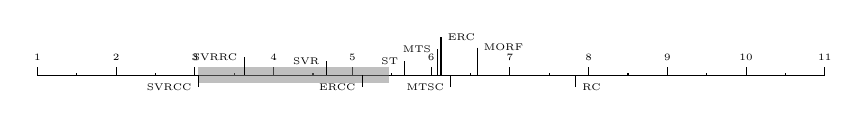
\begin{tikzpicture}
 %axis
 \draw (1,0) -- (11,0);
 \foreach \x in {1,2,3,4,5,6,7,8,9,10,11} {
  \draw (\x, 0) -- ++(0,.1) node [above,scale=0.7] {\tiny \x};
  \ifthenelse{\x < 11}{\draw (\x+.5, 0) -- ++(0,.03);}{}
 }
 % coordinates
 \coordinate (c0) at (3.0417,0);
 \coordinate (c1) at (3.6250,0);
 \coordinate (c2) at (4.6667,0);
 \coordinate (c3) at (5.1250,0);
 \coordinate (c4) at (6.1250,0);
 \coordinate (c5) at (7.8333,0);
 \coordinate (c6) at (6.2500,0);
 \coordinate (c7) at (6.0833,0);
 \coordinate (c8) at (5.6667,0);
 \coordinate (c9) at (6.5833,0);

 % labels
 \node (l0) at (c0) [below left=.025cm and 0cm, align=right,scale=0.7] {\tiny SVRCC};
 \node (l1) at (c1) [above left=.1cm and 0cm, align=right,scale=0.7] {\tiny SVRRC};
 \node (l2) at (c2) [above left=.05cm and 0cm, align=right,scale=0.7] {\tiny SVR};
 \node (l3) at (c3) [below left=.025cm and 0cm, align=left,scale=0.7] {\tiny ERCC};
 \node (l4) at (c4) [above right=.35cm and 0cm, align=right,scale=0.7] {\tiny ERC};
 \node (l5) at (c5) [below right=.025cm and 0cm, align=left,scale=0.7] {\tiny RC};
 \node (l6) at (c6) [below left=.025cm and 0cm, align=right,scale=0.7] {\tiny MTSC};
 \node (l7) at (c7) [above left=.2cm and 0cm, align=left,scale=0.7] {\tiny MTS};
 \node (l8) at (c8) [above left=.05cm and 0cm, align=right,scale=0.7] {\tiny ST};
 \node (l9) at (c9) [above right=.22cm and 0cm, align=right,scale=0.7] {\tiny MORF};

 % CD = 1.4845
 \fill[fill=gray,fill opacity=0.5] (3.0417,-0.1) rectangle (5.4653,0.1);
 
 % connectors
 \foreach \x in {0,...,9} {
  \draw (l\x) -| (c\x);
 };
\end{tikzpicture}}\vspace{-1em}
\captionof{figure}{Bonferroni-Dunn test for MSE}\label{fig:BonfDunnMSE}\vspace{-1.5em}
\captionof{table}{Wilcoxon, Nemenyi, and Holm tests for MSE}\label{tab:statmse}
\scriptsize
\resizebox{0.95\textwidth}{!}{\begin{tabular}{lccccc}
\noalign{\smallskip}\hline\noalign{\smallskip}
SVRCC vs. & Wilcoxon $R^{+}$ & Wilcoxon $R^{-}$ & Wilcoxon $p$-value & Nemenyi $p$-value & Holm $p$-value \\ 
\noalign{\smallskip}\hline\noalign{\smallskip}
MORF & 268.0 & 32.0 & $3.2E^{-4}$ & $5.1E^{-5}$ & $6.3E^{-3}$ \\
ST & 241.0 & 59.0 & $7.9E^{-3}$ & $2.7E^{-3}$ & $1.3E^{-2}$ \\
MTS & 224.0 & 76.0 & $3.4E^{-2}$ & $5.0E^{-4}$ & $1.0E^{-2}$ \\
MTSC & 226.0 & 74.0 & $2.9E^{-2}$ & $2.4E^{-4}$ & $7.1E^{-3}$ \\ 
RC & 263.0 & 37.0 & $6.5E^{-4}$ & 0.0000 & $5.6E^{-3}$ \\  
ERC & 234.0 & 66.0 & $1.5E^{-2}$ & $4.2E^{-4}$ & $8.3E^{-3}$ \\
ERCC & 224.0 & 76.0 & $3.4E^{-2}$ & $1.7E^{-2}$ & $1.7E^{-2}$ \\
SVR & 262.0 & 38.0 & $7.4E^{-4}$ & $6.3E^{-2}$ & $2.5E^{-2}$ \\ 
SVRRC & 245.0 & 55.0 & $5.3E^{-3}$ & $5.1E^{-1}$ & $5.0E^{-2}$\\ 
\noalign{\smallskip}\hline\noalign{\smallskip}
\end{tabular}}
\end{table}
\subsection{Mean Square Error}\label{subsec:mse}
Table~{\ref{tab:mseResults}} shows that our proposed methods perform the best on $15$ out of the $24$ datasets. In this case, SVRCC also performs the best on $11$ versus the $9$ that the competing methods performed better at. The Iman-Davenport statistic, distributed according to the F-distribution with $9$ and $207$ degrees of freedom is $6.57$, with a $p$-value of $3.1E^{-8}$, implying statistically significant differences among the MSE results.

Figure~{\ref{fig:BonfDunnMSE}} shows the mean rank values of each algorithm along with the critical difference value, $2.4236$, for $\alpha = 0.05$. According to the critical difference bar, there are $6$ out of $10$ algorithms beyond that perform significantly worse than our control algorithm, SVRCC. According to the Wilcoxon test, shown in Table~{\ref{tab:statmse}}, SVRCC is shown to have significantly better performance over all algorithms with $p$-value $< 0.05$. The Nemenyi and Holm tests show that SVRCC performs significantly better than $6$ out of the $9$ algorithms with $p$-values $\leq 5.6E^{-3}$ and $\leq 1.7E^{-2}$ respectively, and has an exact confidence of $0.95$ against all others.

\subsection{Average Root Mean Square Error}\label{subsec:armse}
Table~{\ref{tab:armseresults}} shows that our proposed methods perform the best on $18$ out of the $24$ datasets. In this case, SVRCC performs the best on $15$ versus the $6$ that the methods compared performed better at. The Iman-Davenport statistic is $7.6$, with a $p$-value of $1.3E^{-9}$, implying statistically significant differences in the aRMSE results.

Figure~{\ref{fig:BonfDunnaRMSE}} shows the mean rank values of each algorithm along with the critical difference value, $2.4236$, for $\alpha = 0.05$. According to the critical difference bar, there are $7$ out of $10$ algorithms that perform significantly worse than our control algorithm, SVRCC.

According to the Wilcoxon test, shown in Table~{\ref{tab:statarmse}}, SVRCC is shown to have significantly better performance over all algorithms with $p$-value $< 0.01$. The Nemenyi test shows that SVRCC performs significantly better than $7$ out of the $9$ algorithms with $p$-value $\leq 5.6E^{-3}$, while the stricter Holm test shows that it performs significantly better than $8$ out of the $9$ algorithms with $p$-value $\leq 0.05$.
\begin{table}[t!]
\centering \small
\caption{Average Root Mean Square Error (aRMSE) for MT regressors}\label{tab:armseresults}
\resizebox{0.95\textwidth}{!}{\begin{tabular}{l@{\extracolsep{\fill}}ccccccccccc}
\noalign{\smallskip}\hline\noalign{\smallskip}
Datasets &MORF &ST &MTS &MTSC &RC &ERC &ERCC &SVR &SVRRC &SVRCC \\
\noalign{\smallskip}\hline\noalign{\smallskip}
Slump &0.6711 &0.6652 &0.6456 &0.6699 &0.6787 &0.6793 &0.6649 &0.5561 &0.5345 &\textbf{0.5337} &  \\
Polymer &0.5277 &0.5409 &0.5042 &0.5336 &0.5536 &0.5803 &0.5319 &0.4403 &0.4062 &\textbf{0.4060} &  \\
Andro &0.4649 &0.5420 &0.4414 &0.4871 &0.5390 &0.5317 &0.5039 &0.4326 &0.4061 &\textbf{0.3989} &  \\
EDM &0.6372 &0.6715 &0.6705 &0.6729 &0.6722 &0.6704 &0.6721 &0.6449 &0.6411 &\textbf{0.6366} &  \\
Solar Flare 1 &0.9777 &0.9274 &0.9271 &0.9089 &0.8921 &0.9016 &0.9121 &0.8856 &0.8844 &\textbf{0.8801} &  \\
Jura &0.5800 &0.5686 &0.5720 &0.5706 &0.5726 &0.5712 &0.5693 &0.5794 &0.5687 &\textbf{0.5622} &  \\
Enb &0.1212 &0.1166 &0.1237 &0.1214 &0.1272 &0.1253 &0.1140 &0.0981 &0.0914 &\textbf{0.0903} &  \\
Solar Flare 2 &0.8725 &0.8420 &\textbf{0.8127} &0.8305 &0.8313 &0.8300 &0.8304 &0.8418 &0.8349 &0.8345 &  \\
Wisconsin Cancer &0.9290 &0.9163 &0.9158 &0.9187 &\textbf{0.9153} &0.9160 &0.9173 &0.9422 &0.9362 &0.9306 &  \\
California Housing &0.6541 &0.6366 &0.6889 &0.6530 &0.7053 &0.6632 &0.6079 &0.6038 &0.5859 &\textbf{0.5755} &  \\
Stock &0.1643 &0.1830 &0.1774 &0.1790 &0.1790 &0.1777 &0.1739 &0.1357 &0.1329 &\textbf{0.1308} &  \\
SCPF &0.7113 &0.7235 &0.7342 &0.7255 &0.7285 &0.7143 &0.7227 &0.7155 &0.7081 &\textbf{0.7048} &  \\
Puma8NH &0.7855 &0.8139 &0.8114 &0.8307 &0.8196 &0.8202 &0.8203 &\textbf{0.7650} &0.7740 &0.7671 &  \\
Friedman &0.9382 &0.9203 &0.9219 &0.9199 &0.9219 &0.9197 &0.9193 &0.9203 &0.9195 &\textbf{0.9183} &  \\
Puma32H &0.9395 &\textbf{0.8700} &0.8713 &0.8778 &0.8739 &0.8716 &0.8727 &0.9353 &0.9356 &0.9331 &  \\
Water Quality &\textbf{0.8921} &0.9015 &0.9041 &0.9025 &0.9051 &0.9030 &0.8990 &0.9284 &0.9293 &0.9271 &  \\
M5SPEC &0.5707 &0.5324 &0.5761 &0.5515 &0.5347 &0.5339 &0.5376 &0.2745 &0.2744 &\textbf{0.2740} &  \\
MP5SPEC &0.5315 &0.4914 &0.5426 &0.4947 &0.4930 &0.4928 &0.4928 &0.2337 &\textbf{0.2176} &0.2177 &  \\
MP6SPEC &0.5344 &0.4939 &0.5416 &0.4943 &0.4982 &0.4967 &0.4927 &0.2627 &\textbf{0.2460} &0.2497 &  \\
ATP7d &0.5216 &0.4956 &\textbf{0.4752} &0.4765 &0.5194 &0.5024 &0.4824 &0.5141 &0.5066 &0.5018 &  \\
OES97 &0.4652 &0.4634 &0.4635 &0.4622 &0.4643 &0.4644 &0.4627 &0.3794 &0.3768 &\textbf{0.3749} &  \\
Osales &0.7190 &0.6912 &\textbf{0.6496} &0.6615 &0.7591 &0.6772 &0.6515 &0.7212 &0.7343 &0.7121 &  \\
ATP1d &0.4053 &0.3608 &0.3587 &0.3591 &0.3653 &0.3562 &0.3596 &0.3693 &0.3638 &\textbf{0.3507} &  \\
OES10 &0.3954 &0.3896 &0.3897 &0.3892 &0.3901 &0.3903 &0.3889 &0.3085 &0.3039 &\textbf{0.3038} &  \\
\noalign{\smallskip}\hline\noalign{\smallskip}
Average &0.6254 &0.6149 &0.6133 &0.6121 &0.6225 &0.6162 &0.6083 &0.5620 &0.5547 &\textbf{0.5506} &  \\
Ranks &7.3333 &5.7708 &5.8125 &6.0625 &7.6250 &6.0208 &4.8542 &5.0625 &3.9167 &\textbf{2.5417} &  \\
\noalign{\smallskip}\hline
\end{tabular}}
\centering \small
\resizebox{0.95\textwidth}{!}{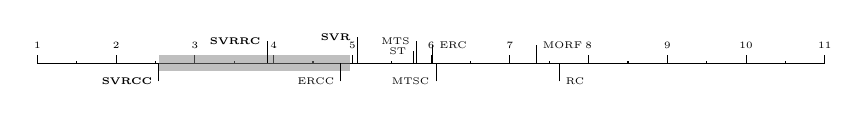
\begin{tikzpicture}
 %axis
 \draw (1,0) -- (11,0);
 \foreach \x in {1,2,3,4,5,6,7,8,9,10,11} {
  \draw (\x, 0) -- ++(0,.1) node [above,scale=0.7] {\tiny \x};
  \ifthenelse{\x < 11}{\draw (\x+.5, 0) -- ++(0,.03);}{}
 }
 % coordinates
 \coordinate (c0) at (2.5417,0);
 \coordinate (c1) at (3.9167,0);
 \coordinate (c2) at (5.0625,0);
 \coordinate (c3) at (4.8542,0);
 \coordinate (c4) at (6.0208,0);
 \coordinate (c5) at (7.6250,0);
 \coordinate (c6) at (6.0625,0);
 \coordinate (c7) at (5.8125,0);
 \coordinate (c8) at (5.7708,0);
 \coordinate (c9) at (7.3333,0);

 % labels
 \node (l0) at (c0) [below left=.1cm and 0cm, align=right,scale=0.7] {\tiny \textbf{SVRCC}};
 \node (l1) at (c1) [above left=.15cm and 0cm, align=right,scale=0.7] {\tiny \textbf{SVRRC}};
 \node (l2) at (c2) [above left=.2cm and 0cm, align=right,scale=0.7] {\tiny \textbf{SVR}};
 \node (l3) at (c3) [below left=.1cm and 0cm, align=left,scale=0.7] {\tiny ERCC};
 \node (l4) at (c4) [above right=.1cm and 0cm, align=right,scale=0.7] {\tiny ERC};
 \node (l5) at (c5) [below right=.1cm and 0cm, align=left,scale=0.7] {\tiny RC};
 \node (l6) at (c6) [below left=.1cm and 0cm, align=right,scale=0.7] {\tiny MTSC};
 \node (l7) at (c7) [above left=.15cm and 0cm, align=left,scale=0.7] {\tiny MTS};
 \node (l8) at (c8) [above left=.025cm and 0cm, align=right,scale=0.7] {\tiny ST};
 \node (l9) at (c9) [above right=.1cm and 0cm, align=right,scale=0.7] {\tiny MORF};

 % CD = 1.4845
 \fill[fill=gray,fill opacity=0.5] (2.5417,-0.1) rectangle (4.9653,0.1);
 
 % connectors
 \foreach \x in {0,...,9} {
  \draw (l\x) -| (c\x);
 };
\end{tikzpicture}}\vspace{-1em}
\captionof{figure}{Bonferroni-Dunn test for aRMSE}\label{fig:BonfDunnaRMSE}\vspace{-1.5em}
\captionof{table}{Wilcoxon, Nemenyi, and Holm tests for aRMSE}\label{tab:statarmse}
\scriptsize
\resizebox{0.95\textwidth}{!}{\begin{tabular}{lccccc}
\noalign{\smallskip}\hline\noalign{\smallskip}
SVRCC vs. & Wilcoxon $R^{+}$ & Wilcoxon $R^{-}$ & Wilcoxon $p$-value & Nemenyi $p$-value & Holm $p$-value \\ 
\noalign{\smallskip}\hline\noalign{\smallskip}
MORF & 286.0 & 14.0 & $1.3E^{-5}$ & 0.0000 & $6.3E^{-3}$ \\
ST & 259.0 & 41.0 & $1.1E^{-3}$ & $2.2E^{-4}$ & $1.3E^{-2}$ \\
MTS & 247.0 & 53.0 & $4.3E^{-3}$ & $1.8E^{-5}$ & $1.0E^{-2}$ \\ 
MTSC & 251.0 & 49.0 & $2.8E^{-3}$ & $5.6E^{-5}$ & $7.1E^{-3}$ \\
RC & 270.0 & 30.0 & $2.4E^{-4}$ & 0.0000 & $5.6E^{-3}$ \\ 
ERC & 255.0 & 45.0 & $1.8E^{-3}$ & $6.9E^{-5}$ & $8.3E^{-3}$ \\
ERCC & 246.0 & 54.0 & $4.8E^{-3}$ & $8.2E^{-3}$ & $2.5E^{-2}$ \\
SVR & 296.0 & 4.00 & $8.3E^{-7}$ & $3.9E^{-3}$ & $1.7E^{-2}$ \\
SVRRC & 284.0 & 16.0 & $2.0E^{-5}$ & $1.2E^{-1}$ & $5.0E^{-2}$ \\
\noalign{\smallskip}\hline\noalign{\smallskip}
\end{tabular}}
\end{table}

\subsection{Average Relative Root Mean Square Error}\label{subsec:arrmse}
\begin{table}[b!]
\centering \small
\caption{Average Relative Root Mean Square Error (aRRMSE) for MT regressors}\label{tab:arrmseresults}
\resizebox{0.95\textwidth}{!}{\begin{tabular}{l@{\extracolsep{\fill}}ccccccccccc}
\noalign{\smallskip}\hline\noalign{\smallskip}
Datasets &MORF &ST &MTS &MTSC &RC &ERC &ERCC &SVR &SVRRC &SVRCC \\
\noalign{\smallskip}\hline\noalign{\smallskip}
Slump &0.6939 &0.6886 &0.6690 &0.6938 &0.7019 &0.7022 &0.6886 &0.5765 &\textbf{0.5545} &0.5560 &  \\
Polymer &0.6159 &0.5971 &0.5778 &0.6493 &0.6270 &0.6544 &0.6131 &0.5573 &0.5253 &\textbf{0.5116} &  \\
Andro &0.5097 &0.5979 &0.5155 &0.5633 &0.5924 &0.5885 &0.5666 &0.4856 &0.4651 &\textbf{0.4455} &  \\
EDM &0.7337 &0.7442 &0.7413 &0.7446 &0.7449 &0.7452 &0.7443 &0.7058 &0.7070 &\textbf{0.6978} &  \\
Solar Flare 1 &1.3046 &1.1357 &1.1168 &1.0758 &0.9951 &1.0457 &1.0887 &0.9917 &0.9455 &\textbf{0.9320} &  \\
Jura &0.5969 &0.5874 &0.5906 &0.5892 &0.5910 &0.5896 &0.5880 &0.5952 &\textbf{0.5764} &0.5885 &  \\
Enb &0.1210 &0.1165 &0.1231 &0.1211 &0.1268 &0.1250 &0.1139 &0.0977 &0.0910 &\textbf{0.0899} &  \\
Solar Flare 2 &1.4167 &1.1503 &\textbf{0.9483} &1.0840 &1.0092 &1.0522 &1.0928 &1.0385 &1.0253 &1.0298 &  \\
Wisconsin Cancer &0.9413 &0.9314 &0.9308 &0.9336 &\textbf{0.9305} &0.9313 &0.9323 &0.9555 &0.9483 &0.9427 &  \\
California Housing &0.6611 &0.6447 &0.6974 &0.6630 &0.7131 &0.6690 &0.6146 &0.6130 &0.5945 &\textbf{0.5852} &  \\
Stock &0.1653 &0.1844 &0.1787 &0.1803 &0.1802 &0.1789 &0.1752 &0.1364 &\textbf{0.1337} &0.1388 &  \\
SCPF &0.8273 &0.8348 &0.8436 &0.8308 &0.8263 &0.8105 &0.8290 &0.8164 &0.8037 &\textbf{0.8013} &  \\
Puma8NH &0.7858 &0.8142 &0.8118 &0.8311 &0.8199 &0.8205 &0.8207 &\textbf{0.7655} &0.7744 &0.7676 &  \\
Friedman &0.9394 &0.9214 &0.9231 &0.9210 &0.9231 &0.9209 &0.9204 &0.9218 &0.9208 &\textbf{0.9196} &  \\
Puma32H &0.9406 &\textbf{0.8713} &0.8727 &0.8791 &0.8752 &0.8729 &0.8740 &0.9364 &0.9367 &0.9319 &  \\
Water Quality &\textbf{0.8994} &0.9085 &0.9109 &0.9093 &0.9121 &0.9097 &0.9057 &0.9343 &0.9310 &0.9045 &  \\
M5SPEC &0.5910 &0.5523 &0.5974 &0.5671 &0.5552 &0.5542 &0.5558 &0.2951 &0.2935 &\textbf{0.2925} &  \\
MP5SPEC &0.5522 &0.5120 &0.5683 &0.5133 &0.5145 &0.5143 &0.5119 &0.2484 &\textbf{0.2323} &0.2358 &  \\
MP6SPEC &0.5553 &0.5152 &0.5686 &0.5119 &0.5198 &0.5187 &0.5109 &0.2850 &0.2669 &\textbf{0.2623} &  \\
ATP7d &0.5563 &0.5308 &\textbf{0.5141} &0.5142 &0.5558 &0.5397 &0.5182 &0.5455 &0.5371 &0.5342 &  \\
OES97 &0.5490 &0.5230 &0.5229 &0.5217 &0.5239 &0.5237 &0.5222 &0.4641 &\textbf{0.4618} &0.4635 &  \\
Osales &0.7596 &0.7471 &\textbf{0.7086} &0.7268 &0.8318 &0.7258 &0.7101 &0.7924 &0.7924 &0.7811 &  \\
ATP1d &0.4173 &0.3732 &0.3733 &0.3712 &0.3790 &\textbf{0.3696} &0.3721 &0.3773 &0.3707 &0.3775 &  \\
OES10 &0.4518 &0.4174 &0.4176 &0.4171 &0.4178 &0.4180 &0.4166 &0.3570 &0.3555 &\textbf{0.3538} &  \\
\noalign{\smallskip}\hline\noalign{\smallskip}
Average &0.6910 &0.6625 &0.6551 &0.6589 &0.6611 &0.6575 &0.6536 &0.6039 &0.5935 &\textbf{0.5893} &  \\
Ranks &7.5000 &5.7708 &5.9375 &6.1667 &7.4375 &6.3750 &4.9792 &4.7708 &3.2708 &\textbf{2.7917} &  \\
\noalign{\smallskip}\hline
\end{tabular}}
\centering \small
\resizebox{0.95\textwidth}{!}{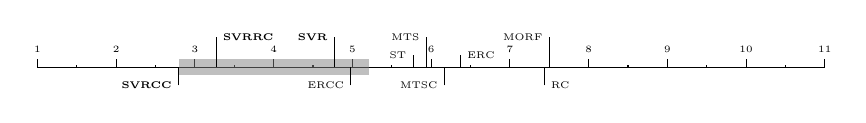
\begin{tikzpicture}
 %axis
 \draw (1,0) -- (11,0);
 \foreach \x in {1,2,3,4,5,6,7,8,9,10,11} {
  \draw (\x, 0) -- ++(0,.1) node [above,scale=0.7] {\tiny \x};
  \ifthenelse{\x < 11}{\draw (\x+.5, 0) -- ++(0,.03);}{}
 }
 % coordinates
 \coordinate (c0) at (2.7917,0);
 \coordinate (c1) at (3.2708,0);
 \coordinate (c2) at (4.7708,0);
 \coordinate (c3) at (4.9792,0);
 \coordinate (c4) at (6.3750,0);
 \coordinate (c5) at (7.4375,0);
 \coordinate (c6) at (6.1667,0);
 \coordinate (c7) at (5.9375,0);
 \coordinate (c8) at (5.7708,0);
 \coordinate (c9) at (7.5000,0);

 % labels
 \node (l0) at (c0) [below left=.1cm and 0cm, align=right,scale=0.7] {\tiny \textbf{SVRCC}};
 \node (l1) at (c1) [above right=.25cm and 0cm, align=right,scale=0.7] {\tiny \textbf{SVRRC}};
 \node (l2) at (c2) [above left=.25cm and 0cm, align=right,scale=0.7] {\tiny \textbf{SVR}};
 \node (l3) at (c3) [below left=.1cm and 0cm, align=left,scale=0.7] {\tiny ERCC};
 \node (l4) at (c4) [above right=.025cm and 0cm, align=right,scale=0.7] {\tiny ERC};
 \node (l5) at (c5) [below right=.1cm and 0cm, align=left,scale=0.7] {\tiny RC};
 \node (l6) at (c6) [below left=.1cm and 0cm, align=right,scale=0.7] {\tiny MTSC};
 \node (l7) at (c7) [above left=.25cm and 0cm, align=left,scale=0.7] {\tiny MTS};
 \node (l8) at (c8) [above left=.025cm and 0cm, align=right,scale=0.7] {\tiny ST};
 \node (l9) at (c9) [above left=.25cm and 0cm, align=right,scale=0.7] {\tiny MORF};

 % CD = 1.4845
 \fill[fill=gray,fill opacity=0.5] (2.7917,-0.1) rectangle (5.2153,0.1);
 
 % connectors
 \foreach \x in {0,...,9} {
  \draw (l\x) -| (c\x);
 };
\end{tikzpicture}}\vspace{-1em}
\captionof{figure}{Bonferroni-Dunn test for aRRMSE}\label{fig:BonfDunnaRRMSE}\vspace{-1.5em}
\captionof{table}{Wilcoxon, Nemenyi, and Holm tests for aRRMSE}\label{tab:statarrmse}
\scriptsize
\resizebox{0.95\textwidth}{!}{\begin{tabular}{lccccc}
\noalign{\smallskip}\hline\noalign{\smallskip}
SVRCC vs. & Wilcoxon $R^{+}$ & Wilcoxon $R^{-}$ & Wilcoxon $p$-value & Nemenyi $p$-value & Holm $p$-value \\ 
\noalign{\smallskip}\hline\noalign{\smallskip}
MORF & 290.0 & 10.0 & $5.1E^{-6}$ & $0.0000$ & $5.6E^{-3}$ \\  
ST & 261.0 & 39.0 & $8.5E^{-4}$ & $6.5E^{-4}$ & $1.3E^{-2}$\\
MTS & 239.0 & 61.0 & $9.6E^{-3}$ & $3.2E^{-3}$ & $1.0E^{-2}$\\ 
MTSC & 261.0 & 39.0 & $8.5E^{-4}$ & $1.1E^{-3}$ & $8.3E^{-3}$\\  
RC & 275.0 & 25.0 & $1.1E^{-4}$ & 0.0000 & $6.3E^{-3}$ \\
ERC & 261.0 & 39.0 & $8.5E^{-4}$ & $4.1E^{-5}$ & $7.1E^{-3}$\\ 
ERCC & 254.0 & 46.0 & $2.0E^{-3}$ & $1.2E^{-2}$ & $1.7E^{-2}$\\
SVR & 291.0 & 9.00 & $3.9E^{-6}$ & $2.4E^{-2}$ & $2.5E^{-2}$\\
SVRRC & 222.5 & 77.5 & $3.8E^{-2}$ & $5.8E^{-1}$ & $5.0E^{-2}$ \\ 
\noalign{\smallskip}\hline\noalign{\smallskip}
\end{tabular}}
\end{table}
Table~{\ref{tab:arrmseresults}} shows that our proposed methods perform the best on $16$ out of the $24$ datasets. In this case, SVRCC performs the best on $11$ versus the $6$ that the competing methods performed better at. The Iman-Davenport statistic is $8.54$, with a $p$-value of $7.6E^{-11}$.

Figure~{\ref{fig:BonfDunnaRRMSE}} shows the mean rank values of each algorithm along with the critical difference value, $2.4236$, for $\alpha = 0.05$. According to the critical difference bar, there are $6$ out of $10$ algorithms beyond that perform significantly worse than our control algorithm, SVRCC.

According to the Wilcoxon test, shown in Table~{\ref{tab:statarrmse}}, SVRCC is shown to have significantly better performance over all algorithms with $p$-value $< 0.05$, and $8$ out of the $9$ algorithms for $p$-value $< 0.01$. The Nemenyi test shows that SVRCC performs significantly better than $6$ out of the $9$ algorithms with $p$-value $\leq 5.6E^{-3}$, and the Holm test shows its performance is significantly better than $8$ out of the $9$ algorithms with $p$-value $\leq 0.05$.

\subsection{Run Time}\label{subsec:time}
\begin{table}[t!]
\centering \small
\caption{Run Time (seconds) for MT regressors}\label{tab:timeresults}
\resizebox{0.95\textwidth}{!}{\begin{tabular}{l@{\extracolsep{\fill}}rrrrrrrrrrr}
\noalign{\smallskip}\hline\noalign{\smallskip}
Datasets &MORF &ST &MTS &MTSC &RC &ERC &ERCC &SVR &SVRRC &SVRCC \\
\noalign{\smallskip}\hline\noalign{\smallskip}
Slump &38.1 &2.6 &9.9 &15.9 &1.8 &11.1 &50.5 &\textbf{0.6} &1.9 &0.7 &  \\
Polymer &7.6 &2.7 &9.1 &15.5 &1.9 &14.9 &80.5 &\textbf{0.5} &2.6 &\textbf{0.5} &  \\
Andro &25.7 &4.4 &15.0 &34.2 &3.4 &33.2 &197.9 &\textbf{1.1} &6.2 &\textbf{1.1} &  \\
EDM &24.8 &2.8 &9.4 &18.1 &2.1 &5.8 &19.0 &\textbf{0.9} &1.0 &\textbf{0.9} &  \\
Solar Flare 1 &34.1 &3.5 &13.6 &26.7 &2.7 &17.7 &86.9 &\textbf{2.3} &9.3 &2.6 &  \\
Jura &64.3 &7.9 &31.8 &74.3 &6.4 &43.5 &254.2 &\textbf{4.7} &18.7 &5.3 &  \\
Enb &71.4 &6.6 &26.1 &63.6 &\textbf{5.4} &15.6 &69.6 &11.3 &17.7 &15.9 &  \\
Solar Flare 2 &55.4 &7.4 &30.7 &68.0 &\textbf{6.3} &42.9 &241.5 &9.4 &53.5 &15.6 &  \\
Wisconsin Cancer &51.4 &6.1 &21.9 &53.7 &4.9 &14.8 &61.6 &\textbf{2.0} &2.4 &\textbf{2.0} &  \\
California Housing &93.0 &9.7 &34.8 &75.9 &\textbf{8.2} &21.3 &102.0 &15.8 &25.2 &23.6 &  \\
Stock &93.7 &11.7 &46.8 &96.7 &\textbf{11.0} &75.4 &427.3 &18.5 &90.5 &26.3 &  \\
SCPF &66.3 &19.3 &65.9 &176.3 &\textbf{15.0} &104.2 &734.2 &32.8 &162.8 &48.8 &  \\
Puma8NH &130.4 &29.7 &106.7 &288.6 &\textbf{27.9} &201.6 &1227.7 &94.1 &516.6 &177.1 &  \\
Friedman &79.5 &27.0 &81.2 &258.3 &25.0 &273.7 &2871.6 &\textbf{12.3} &322.3 &18.8 &  \\
Puma32H &93.9 &68.1 &181.0 &635.0 &87.7 &667.9 &6087.0 &\textbf{32.2} &1018.7 &53.1 &  \\
Water Quality &108.4 &\textbf{93.1} &262.1 &912.3 &127.2 &925.4 &10993.3 &110.2 &2567.9 &189.5 &  \\
M5SPEC &89.8 &68.9 &166.3 &604.6 &73.7 &262.3 &3132.1 &\textbf{39.2} &546.7 &45.1 &  \\
MP5SPEC &84.5 &94.6 &221.2 &888.3 &91.5 &557.0 &6864.1 &\textbf{49.3} &1132.1 &58.4 &  \\
MP6SPEC &90.3 &93.4 &212.6 &871.0 &89.1 &557.6 &6761.3 &\textbf{47.2} &1227.1 &58.5 &  \\
ATP7d &\textbf{70.5} &262.6 &452.1 &2319.8 &242.1 &1779.2 &24373.8 &80.0 &1897.4 &136.5 &  \\
OES97 &\textbf{83.4} &485.3 &1146.6 &4928.9 &499.8 &5315.0 &58072.1 &148.2 &3759.1 &342.6 &  \\
Osales &\textbf{92.0} &1094.8 &2340.7 &8322.2 &986.5 &11361.2 &122265.3 &437.0 &4830.1 &843.6 &  \\
ATP1d &\textbf{70.7} &272.9 &476.5 &2568.9 &261.9 &2138.9 &26768.9 &95.0 &2127.8 &174.4 &  \\
OES10 &\textbf{90.0} &738.9 &1633.6 &6682.9 &688.5 &7150.8 &83533.1 &229.1 &5419.4 &577.1 &  \\
\noalign{\smallskip}\hline\noalign{\smallskip}
Average &71.2 &142.2 &316.5 &1250.0 &136.2 &1316.3 &14803.2 &\textbf{61.4} &1073.2 &117.4 &  \\
Ranks &5.5 &3.71 &6.0 &8.29 &3.0 &7.08 &9.92 &\textbf{1.88} &6.71 &2.92 &  \\
\noalign{\smallskip}\hline
\end{tabular}}
\centering \small
\resizebox{0.95\textwidth}{!}{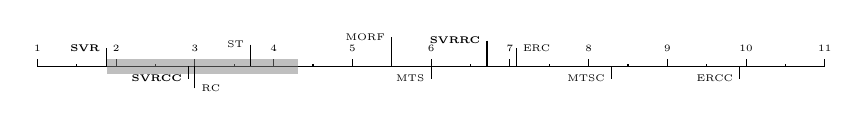
\begin{tikzpicture}
 %axis
 \draw (1,0) -- (11,0);
 \foreach \x in {1,2,3,4,5,6,7,8,9,10,11} {
  \draw (\x, 0) -- ++(0,.1) node [above,scale=0.7] {\tiny \x};
  \ifthenelse{\x < 11}{\draw (\x+.5, 0) -- ++(0,.03);}{}
 }
 % coordinates
 \coordinate (c0) at (2.92,0);
 \coordinate (c1) at (6.71,0);
 \coordinate (c2) at (1.88,0);
 \coordinate (c3) at (9.92,0);
 \coordinate (c4) at (7.08,0);
 \coordinate (c5) at (3,0);
 \coordinate (c6) at (8.29,0);
 \coordinate (c7) at (6,0);
 \coordinate (c8) at (3.71,0);
 \coordinate (c9) at (5.5,0);

 % labels
 \node (l0) at (c0) [below left=.025cm and 0cm, align=right,scale=0.7] {\tiny \textbf{SVRCC}};
 \node (l1) at (c1) [above left=.2cm and 0cm, align=right,scale=0.7] {\tiny \textbf{SVRRC}};
 \node (l2) at (c2) [above left=.1cm and 0cm, align=right,scale=0.7] {\tiny \textbf{SVR}};
 \node (l3) at (c3) [below left=.025cm and 0cm, align=left,scale=0.7] {\tiny ERCC};
 \node (l4) at (c4) [above right=.1cm and 0cm, align=right,scale=0.7] {\tiny ERC};
 \node (l5) at (c5) [below right=.15cm and 0cm, align=left,scale=0.7] {\tiny RC};
 \node (l6) at (c6) [below left=.025cm and 0cm, align=right,scale=0.7] {\tiny MTSC};
 \node (l7) at (c7) [below left=.025cm and 0cm, align=left,scale=0.7] {\tiny MTS};
 \node (l8) at (c8) [above left=.15cm and 0cm, align=right,scale=0.7] {\tiny ST};
 \node (l9) at (c9) [above left=.24cm and 0cm, align=right,scale=0.7] {\tiny MORF};

 % CD = 1.4845
 \fill[fill=gray,fill opacity=0.5] (1.88,-0.1) rectangle (4.3036,0.1);
 
 % connectors
 \foreach \x in {0,...,9} {
  \draw (l\x) -| (c\x);
 };
\end{tikzpicture}}\vspace{-1em}
\captionof{figure}{Bonferroni-Dunn test for Run Time}\label{fig:BonfDunnTime}\vspace{-1.5em}
\captionof{table}{Wilcoxon, Nemenyi, and Holm tests for Run Time}\label{tab:stattime}
\scriptsize
\resizebox{0.95\textwidth}{!}{\begin{tabular}{lccccc}
\noalign{\smallskip}\hline\noalign{\smallskip}
SVRCC vs. & Wilcoxon $R^{+}$ & Wilcoxon $R^{-}$ & Wilcoxon $p$-value & Nemenyi $p$-value & Holm $p$-value \\ 
\noalign{\smallskip}\hline\noalign{\smallskip}
SVRCC & 295.0 & 5.00 & $1.2E^{-6}$ &  $2.3E^{-1}$ & $5.0E^{-2}$\\ 
MORF & 225.0 & 75.0 & $3.2E^{-2}$ &  $3.4E^{-5}$ & $1.3E^{-2}$\\  
ST & 221.5 & 78.5 & $4.1E^{-2}$ &  $3.6E^{-2}$ & $1.7E^{-2}$\\   
MTS & 300.0 & 0.00 & $1.2E^{-7}$ &  $2.0E^{-6}$ & $1.0E^{-2}$\\ 
MTSC & 300.0 & 0.00 & $1.2E^{-7}$ &  0.0000 & $6.3E^{-3}$\\
RC & 229.0 & 71.0 & $2.3E^{-2}$ &  $2.0E^{-1}$ & $2.5E^{-2}$ \\  
ERC & 300.0 & 0.00 & $1.2E^{-7}$ & 0.0000 & $7.1E^{-3}$\\  
ERCC & 300.0 & 0.00 & $1.2E^{-7}$ & 0.0000 & $5.6E^{-3}$\\ 
SVRRC & 300.0 & 0.00 & $1.2E^{-7}$ &  0.0000 & $8.3E^{-3}$\\ 
\noalign{\smallskip}\hline\noalign{\smallskip}
\end{tabular}}
\end{table}
Table~{\ref{tab:timeresults}} shows that our proposed methods perform faster on $16$ out of the $24$ datasets. In this case, SVR performs the best on $12$ versus the $6$ of the state-of-the-art methods. The Iman-Davenport statistic $64.41$, with a $p$-value of $0.0$ which implies a statistical confidence of $100\%$. Figure~{\ref{fig:BonfDunnTime}} shows the mean rank values of each algorithm along with the critical difference value, $2.4236$, for $\alpha = 0.05$. According to the critical difference bar, there are $6$ out of $10$ algorithms beyond that perform significantly worse than our control algorithm, SVR.
According to the Wilcoxon test, shown in Table~{\ref{tab:stattime}}, SVR is shown to have significantly better performance over all algorithms with $p$-value $< 0.01$. The Nemenyi and Holm tests show that SVRCC performs significantly better than $6$ out of the $9$ algorithms and $8$ out of the $9$ algorithms with $p$-value $\leq 5.6E^{-3}$ and $p$-value $\leq 1.6E^{-2}$, respectively.

\subsection{Discussion}\label{sec:discussion}
Results indicate that our proposed methods perform competitively against the current contemporary methods, specifically SVRCC which exploits relationships among the targets. Firstly, they show that using SVR as a base-line method for multi-target chaining causes a performance improvement in model prediction, compared to other ST base-line models, as well as most MT methods. This demonstrates the advantages of using the SVR method as a base-line for multi-target learning, thus increasing the performance of the ensemble of regressor chains, SVRRC, compared to ERCC. More importantly, the results highlight the major advantage of capturing and exploiting the targets' relationships during model training. Using an ensemble of randomly generated chains does not ensure the targets' correlations are fully captured; however, using a maximum correlation chain improves the performance in terms of quality metrics as well as run time. The run time of SVR was shown to be the fastest, due to the fact that its complexity is mostly dependent on the number of targets. However, this method does not consider any of the correlations that might exist among the target variables, but SVRCC does take them into account and does not have a significant impact on run time. The most noteworthy finding that highlights advantage of using the base-line SVR and the maximum correlation method, SVRCC, rather than random chaining as done in ERCC, are the run time results and their analysis. ERCC had the worst run time across all datasets, whereas our proposals, SVR and SVRCC, performed the fastest. This emphasizes the advantage of using a single chain rather an ensemble of random chains, especially when the single chain is ordered in the direction of the targets maximum correlation.

\section{Conclusions}\label{sec:MTRconclusions}
This contribution proposed three novel methods for solving multi-target regression problems. The first method takes a \textit{problem transformation} approach, which generates $m$ ST models, each trained independently. This base-line approach was shown to perform the best in terms of run time, but its drawback  is that it does not take the possible correlations between the target variables into account during training. The second implements SVR as an ensemble model of randomly generated chains, inspired by the classification method ERCC. This was done to investigate the effects of exploiting correlations among the target variables during model training. Due to the random nature of this method, capturing target correlations is not guaranteed. The third proposal, SVRCC, generates a single chain that is ordered in the direction of the targets' maximum correlation, ensuring the correlations among targets are taken into account within the learning process.

The experimental study compared the proposed methods' performances to $7$ popular, contemporary methods on 24 MT regression datasets. Firstly, the results show the superior performance of using the SVR method as a base-line model, rather than regression trees as used in MORF. The results for SVRRC show an increase in performance when random chaining is used to develop an ensemble model. This indicates the importance of the relationship among the target variables during training. Finally, the results show the superiority of using the SVRCC method, which was ranked the best in all quality metrics and second best in terms of run time. SVRCC performed better than the single-target SVR model and the randomly chained ensemble model SVRRC, showing that the targets' maximum correlation does positively contribute toward model training. The statistical analysis supports and shows the significance of the results obtained by our experiments. They demonstrated that statistically significant differences exist between the proposed algorithms against the methods compared. SVRCCs competitive performance, as well as speed, shows that it is a powerful learning algorithm for multi-target problems. The research outcomes of this chapter have been published in~\cite{melki2017multi}.

\chapter{Multi-Instance SVM using Bag-Representatives \label{chap:mirsvm}}
This contribution proposes a novel support vector machine multiple-instance formulation and presents an algorithm with a bag-representative selector that trains the SVM based on bag-level information, named MIRSVM. The contribution is able to identify instances that highly impact classification, i.e. bag-representatives, for both positive and negative bags, while finding the optimal class separation hyperplane. Unlike other multi-instance SVM methods, this approach eliminates possible class imbalance issues by allowing both positive and negative bags to have at most one representative, which constitute as the most contributing instances to the model. The experimental study evaluates and compares the performance of this proposal against $11$ popular multi-instance methods over $15$ datasets, and the results are validated through non-parametric statistical analysis. The results indicate that bag-based learners outperform the instance-based and wrapper methods, and this proposal's overall superior performance against other multi-instance SVM models. 

\section{Multi-Instance Classification Background}\label{sec:mibackground}
This section defines the notation that will be used throughout the paper, and reviews related works on multi-instance learning and multi-instance support vector machines.

\subsection{Notation}\label{subsec:minotation}
Let $\mathcal{D}$ be a training dataset of $n$ bags. Let $\bm{Y} \in \mathcal{D}$ be a vector of $n$ labels corresponding to each bag, having a domain of $\bm{Y} \in \set{-1,1}^n$. Let $\bm{X} \in \mathcal{D}$ be a matrix consisting of $d$ input variables and $m$ instances, $\bm x_i \in \bm X,\, \forall i \in \set{1,\ldots,m}$ , having a domain of $\bm{X} \in \mathbb{R}^{m \times d}$. Let $\mathcal{B}$ be the set of bags which contain $|\mathcal{B}_I|$ number of instances, sometimes of different size and usually non-overlapping, such that $\mathcal{B}_I = \{\bm x_{1}, \ldots, \bm x_{|\mathcal{B}_I|}\}$ for index set $I \in \set{1,\ldots,n}$. 

\subsection{Multi-Instance Classification}
The difference between MIL and traditional learning is the nature of the data. In the traditional binary classification setting, the goal is to learn a model that maps input samples to labels, $f: \reals^{m \times d} \rightarrow Y^m \in \set{-1,\,+1}$. In the multi-instance setting, samples are called \textit{bags} and each bag contains one or more input instances and is assigned a single bag-level label. Input instances, $\set{\bm x_1,\, \bm x_2,\, \ldots,\, \bm x_m}$, are grouped into bags with unique identifiers, $\mathcal{B} = \set{\mathcal{B}_1,\, \mathcal{B}_2,\, \ldots,\, \mathcal{B}_n \st \mathcal{B}_I = \set{\bm x_i \st \forall i \in I},\, \forall I \in \set{1, \ldots, n}}$ and assigned a label, $Y_I$. The individual instance labels within a bag are unknown. Using the training dataset $\mathcal{D} = \{(\mathcal{B}_1,Y_1), \ldots, (\mathcal{B}_n,Y_n)\}$, the goal is to train a classifier that predicts the label of an unseen bag, $f(\mathcal{B}_{n+1}) \rightarrow Y_{n+1}$~\cite{Amores2013}. 

In order to build a classifier without any knowledge of the individual training instance labels, Dietterich et. al.~\cite{Dietterich1997} proposed the \textit{standard MI} (SMI) hypothesis, shown in Equation~\eqref{eqn:stas}, which states that a bag is labeled positive if and only if at least one of the instances in the bag is positive, and is labeled negative otherwise.
\begin{equation}
\centering \label{eqn:stas}
 Y_I = \begin{cases}
			+1 & \text{if }\exists\, y_i = +1,\, \forall i \in I \\
			-1 & \text{otherwise}.
		  \end{cases}
\end{equation}

This implies that individual instance labels $y_i$ exist, but are not known (for positive bags) during training. Equation~\eqref{eqn:stas} can also be rewritten as Equation~\eqref{eqn:stasmax} for simplicity:
\begin{equation}
\centering \label{eqn:stasmax}
Y_I = \text{argmax}_{\forall i \in I}\,\,\, y_i.
\end{equation}

In addition to the SMI assumption, alternative MI assumptions have been proposed to date~\cite{Foulds2010}. A recent review~\cite{Amores2013} describing the taxonomy of multi-instance classification presents various methods and algorithms used in literature which are categorized based on their approach to handling the MI input space. Instance-based classifiers that fall under the \textit{instance-space paradigm}, aim to separate instances in positive bags from those in negative ones. Bag-level classifiers (\textit{bag-space paradigm}) treat each bag as a whole entity, implicitly extracting information from each bag in order to accurately predict their labels. Methods that fall under the \textit{embedded-space paradigm} map the input bags to a single feature vector that explicitly encapsulates all the relevant information contained within each bag.

Instance-based methods that follow the SMI assumption attempt to identify desirable instance properties that make a bag positive. One traditional method in this category is the Axis-Parallel Rectangle (APR)~\cite{Dietterich1997}, which trains a model that assigns a positive label to an instance if it belongs to an axis-parallel rectangle in feature space, and assigns a negative label otherwise. The APR is optimized by maximizing the number of positive bags in the training set containing at least one instance in the APR, while concurrently maximizing the number of negative bags that do not contain any instance in the APR. Another similar method is the Diverse Density (DD)~\cite{Maron1998} framework which is maximized for instances in feature space that are near at least one instance in a positive bag and far from all instances in negative bags. In the Expectation-Maximization Diverse Density (EM-DD) algorithm, Zhang and Goldman~\cite{Zhang2001} propose a similar framework that iteratively maximizes the DD measure. Auer and Ortner~\cite{Auer2004} present a boosting approach that uses balls centered around positive bags to solve the MI problem called Multi-Instance Optimal Ball (MIOptimalBall). This approach is similar to that of APR and DD, except that Auer and Ortner~\cite{Auer2004} propose computing optimal balls per positive bags. A major challenge affecting these methods is that the distributions of the positive and negative bags affect their performance. Methods based on the DD metric~\cite{Carbonneau2016,Chen2006,Chen2004} assume the positive instances form a cluster, which may not be the case. Alternatively, Fu et al.\cite{Fu2011} models the distribution of negative bags with Gaussian kernels, which can prove difficult when the quantity of data is limited.

Some methods in literature, such as Simple-MI~\cite{Dong2006}, transform the MI dataset to a traditional instance-level dataset. Simple-MI represents each bag with the mean vector of the instances within it. The major disadvantage of these types of approaches is that they assume the distribution the instances in positive bags is positive, when it may not be.

An extension of traditional single-instance $k$-nearest neighbors method (KNN) was proposed by Wang and Zucker~\cite{Wang2000} to be applied to the bag-level, named CitationKNN. This method uses a distance function between bags in order to determine bag similarities. Not only are the set of closest bags to a single bag  considered, but also how many bags is the single bag closest to. A voting scheme is then used to determine the bag class labels.

Blockeel et al.~\cite{Blockeel2005} introduced the Multi-Instance Tree Inducer (MITI), based on the standard MI assumption, which uses decision trees as a heuristic to solve the MI problem. This approach aims to identify whether an instance within a bag is truly positive and eliminate false positives within the same bag. The disadvantage of this approach stems from removing instances considered as false positives from partially grown trees without updating the existing tree structure. Bjerring and Frank~\cite{Bjerring2011} then enhanced this approach by creating the method Multi-Instance Rule Induction (MIRI). The algorithm aims to eliminate any possibility of a suboptimal split because the tree is discarded and regrown. Other popular methods include MIBoost~\cite{Hall2009}, MIWrapper~\cite{Frank2003}, and Two-Level Classifier (TLC)~\cite{Wang2014}.

The MI adaptation of the SVM presents two contexts for solving the problem: the instance-level and the bag-level. The first tries to identify instances, either all within a bag or just key instances, that help find the optimal separating hyperplane between positive and negative bags. The latter uses kernels defined over whole bags to optimize the margin~\cite{Doran201479}. 

Andrews et. al.~\cite{Andrews2002} proposed a mixed-integer quadratic program that solves the MI problem at an instance-level, using a support vector machine, named MISVM, that can be solved heuristically. Rather than maximizing the margin of separability between instances of different classes, this instance-based method maximizes the margin between bags. It tries to identify the key instance from each positive bag that makes the bag positive by assuming it has the highest margin value. Instances from positive bags are selected as bag-representatives, and the algorithm iteratively creates a classifier that separates those representatives from all instances from the negative bags. Using bag-representatives from one class and all instances from the other is an example of an approach that combines rules from the SMI assumption and the collective assumption. A disadvantage of this approach stems from the assumption that all instances within positive bags are also positive, which is an implicit step in the initialization of MISVM. Andrews et. al.~\cite{Andrews2002} also proposed a second mixed-integer instance-level approach, named mi-SVM, which does not discard the negative instances of the positive bags. It rather tries to identify the instances within positive bags that are negative and utilize them in the construction of the negative margin. The main disadvantage of these approaches is that they create an imbalanced class problem that favors the negative class, resulting in a biased classifier.

One of the first bag-level approaches to the multi-instance SVM problem was proposed by G{\"a}rtner et. al.~\cite{Smola2002}, who defined a bag-level kernel. A bag-level kernel determines the similarity between two bags in a higher dimensional space. Blaschko et. al.~\cite{Blaschko2006} proposed conformal kernels which manipulate each attribute's dimension based on its importance, without affecting the angles between vectors in the transformed space. These type of bag level kernels transform the bags into a single-instance representation which enables standard SVMs to be directly applied to multi-instance data. 

For most of the methods described above, implicit or explicit assumptions have been made about the distribution of the data. Selecting a method that is robust for a problem such as MIL can be difficult when little is known about the nature of the data, especially considering the unknown distribution of the instances within bags~\cite{Amores2013}. The proposed method, MIRSVM, is a general method that uses support vector machines to design a MIL model without making prior assumptions about the data. Classifiers of this type are known to provide better generalization capabilities and performance, as well as sparser models.

\section{Novel SVM for Multi-Instance Classification}
MIRSVM is based on the idea of selecting representative instances from both positive and negative bags which are used to find an unbiased, optimal separating hyperplane. A representative is iteratively chosen from each bag, and a new hyperplane is formed according to the representatives until they converge. Based on the SMI hypothesis, only one instance in a bag is required to be positive for the bag to adopt a positive label. Due to the unknown distribution of instances within positive bags, MIRSVM is designed to give preference to negative bags during training, because their distribution is known, i.e. all instances are guaranteed to be negative. This is evident during the representative selection process, by taking the index of the maximum output value within each bag based on the current hyperplane using the following rule, $s_I = \text{argmax}_{i \in I} (\langle \bm w,\, \bm x_i \rangle + b),\, \forall I \in \set{1,\ldots,n}$. In other words, the most positive instance is chosen from each positive bag and the least negative instance is chosen from each negative bag (instances with the largest output value based on the current hyperplane), pushing the decision boundary  towards the positive bags. Equation~\eqref{eq:primalmirsvm} presents the primal MIRSVM optimization problem:
\begin{subequations} 
\label{eq:primalmirsvm}
\begin{alignat}{2}
\min\limits_{\bm w, b,\bm\xi}& {\,\,} \frac{1}{2}||\bm{w}||^2 + \frac{C}{n}\sum_I \xi_I, \tag{\ref{eq:primalmirsvm}}\\ 
\text{s.t.}& {\,\,} Y_I(\langle\bm{w},\bm x_{s_I}\rangle + b) \geq 1 - \xi_I,\, \forall I \in \set{1,\ldots,n}  \label{eq:primalmirsvm1}\\
{} & {\,\,} \xi_I \geq 0,\, \forall I \in \set{1,\ldots,n}, 
\end{alignat}
\end{subequations} 
where $\bm S_I$ is the set of the bag representatives' indices and $\bm x_{s_I}$ is the instance representative of bag $\mathcal{B}_I$. Note the variables in MIRSVMs formulation are the similar to those of the traditional SVM, except they are now representing each bag as an instance. Solving the optimization problem given in Equation~\eqref{eq:primalmirsvm} using a quadratic programming solver is a computationally expensive task due to the number of constraints, which scales by the number of bags $n$, as well as the calculation of the inner product between two $d$-dimensional vectors in constraint~\eqref{eq:primalmirsvm1}. The proposed solution for these problems was deriving and solving the dual of the optimization problem given by Equation~\eqref{eq:primalmirsvm}. 

The dual can be formed by taking the Lagrangian of~\eqref{eq:primalmirsvm}, given by Equation~\eqref{eqn:svmlagrangian}, where $\bm \alpha$ and $\bm \beta$ are the non-negative Lagrange multipliers.
\begin{equation}
\centering \label{eqn:svmlagrangian}
\resizebox{.9\textwidth}{!}{$
\begin{aligned}
\mathcal{L}\left(\bm{w},b,\bm{\xi},\bm{\alpha},\bm{\beta}\right) = \frac{1}{2}\sum_{j=1}^d w_j^2  + \frac{C}{n}\sum_I \xi_I - \sum_I{\beta_I \xi_I} - \sum_I{\alpha_I\left(Y_I\left(\sum_{j=1}^d w_j x_{s_Ij} + b\right) -1 + \xi_I\right)}
\end{aligned}$} 
\end{equation}

At optimality~\cite{Boyd2004}, $\bigtriangledown_{w,b,\xi}\mathcal{L}(\bm{w},b,\bm{\xi},\bm{\alpha},\bm{\beta}) = 0$ and the following conditions are met:
\begin{align}
&\frac{\partial\mathcal{L}}{\partial w_j}: w_j = \sum_I{\alpha_I\,Y_I\, x_{s_I\,j}},\,\forall j \in \{1,\ldots,d\}\label{eqn:optcond1}\\
&\frac{\partial\mathcal{L}}{\partial b}: \sum_I{\alpha_IY_I} = 0,\label{eqn:optcond2}\\
&\frac{\partial\mathcal{L}}{\partial\xi_I}: \alpha_I + \beta_I = \frac{C}{n},\,\forall I \in \set{1,\ldots,n}\label{eqn:optcond3} 
\end{align}

By substituting Equations~\eqref{eqn:optcond1},~\eqref{eqn:optcond2}, and~\eqref{eqn:optcond3} into the Lagrangian in~\eqref{eqn:svmlagrangian}, the dual MIRSVM formulation becomes the following:
\begin{subequations} 
\label{eq:dualmirsvm1}
\begin{alignat}{2}
\max\limits_{\bm \alpha,\bm \beta}& \sum_I \alpha_I -\frac{1}{2}\sum_I \sum_{K\in I} \sum_{j=1}^d \alpha_I \alpha_K Y_I Y_K  x_{s_I j} x_{s_K j} \tag{\ref{eq:dualmirsvm1}}\\
\text{s.t.}&  \sum_I{\alpha_IY_I} = 0\, \\
{} & \alpha_I + \beta_I = \frac{C}{n},\,\forall I \in \set{1,\ldots,n}   \label{eq:implicit1}\\
{} & \alpha_I \geq 0,\, \forall I \in \set{1,\ldots,n}  \label{eq:implicit2} \\
{} & \beta_I \geq 0,\, \forall I \in \set{1,\ldots,n},  \label{eq:implicit3}
\end{alignat}
\end{subequations} 
where $s_I$ is computed for each bag, as shown in Equation~\eqref{eq:si}:
\begin{equation}
\label{eq:si}
\centering
s_I = \underset{i \in I}{\text{argmax}}(\sum_{K\in I} \sum_{j=1}^d \alpha_K Y_K x_{s_K j} x_{ij} + b),\, \forall I \in \set{1,\ldots,n}.
\end{equation}

The implicit constraints~\eqref{eq:implicit1} through~\eqref{eq:implicit3} imply three possible cases for $\alpha_I$ values:
\begin{itemize}
\item[1.] If $\alpha_I = 0$, then $\beta_I = C/n$ and $\xi_I = 0$, implying the instance is correctly classified and outside the margin. 
\item[2.] If $0 < \alpha_I < C/n$, then $\beta_I > 0$ and $\xi_I = 0$, indicating that the instance sits on the margin boundary, i.e. is an \textit{unbounded support vector}.
\item[3.] If $\alpha_I = C/n$, then $\beta_I = 0$ and there is no restriction for $\xi_I \geq 0$. This also indicates that the instance is a support vector, but one that is \textit{bounded}. If $0 \leq \xi_I < 1$, then the instance is correctly classified, and is misclassified otherwise. 
\end{itemize}

The dual is then kernelized by replacing the inner product of samples in feature space with their corresponding kernel value, $\spa{K}\left(\bm{x}_{s_I},\bm{x}_{s_K}\right)$. The dual function is now written as:
\begin{subequations} 
\label{eq:dualmirsvm}
\begin{alignat}{2}
\max\limits_{\bm \alpha}& \sum_I \alpha_I - \frac{1}{2}\sum_I \sum_{K\in I} \alpha_I \alpha_K Y_I Y_K  \spa{K}\left(\bm{x}_{s_I},\bm{x}_{s_K}\right) \tag{\ref{eq:dualmirsvm}}\\
\text{s.t.}&  \sum_I{\alpha_IY_I} = 0\,  \\
{} & 0 \leq \alpha_I \leq \frac{C}{n},\, \forall I \in \set{1,\ldots,n}.
\end{alignat}
\end{subequations} 

One of the biggest advantages of the dual SVM formulation is the sparseness of the resulting model. This is because support vectors, instances that have their corresponding $\alpha_I \neq 0$, are only considered when forming the decision boundary. MIRSVM uses a Gaussian RBF kernel, given by Equation~\eqref{eq:gaussiankernel}, where $\sigma$ is the Gaussian shape parameter.
\begin{equation}
\label{eq:gaussiankernel}
\centering
\mathcal{K}(\bm x_i, \bm x_j) = e^{-\frac{\norm{\bm x_i - \bm x_j}^2}{2\sigma^2}}
\end{equation}

To evaluate the output vector, $\bm o_I$, of bag $I$ using the kernel, the following equation is used, where $\mathcal{B}_I$ are the instances of bag $I$, $\bm X_S$ are the optimal bag representatives, and $\bm Y_S$ are the representative bag labels.
\begin{align}
\bm o_I = \spa{K}(\mathcal{B}_I,\bm X_S)*(\bm\alpha \cdot \bm Y_S) + b
\end{align}

The bias term $b$ is calculated as shown in Equation~\eqref{eqn:bias}, where $\bm{sv}$ is the vector of support vector indices and $n_{sv}$ is the number of support vectors~\cite{Huang2006}.
\begin{align}
\label{eqn:bias}
b = \frac{1}{n_{\bm{sv}}}\sum_{\bm{sv}} Y_{\bm{sv}} - \spa{K}(\bm X_{\bm{sv}},\bm X_{\bm{sv}})*(\bm \alpha_{\bm{sv}}\bm\cdot Y_{\bm{sv}})
\end{align}
Algorithm~\ref{alg:mirsvm} shows the procedure for training the multi-instance representative SVM classifier and obtaining the optimal representatives from each bag.  During training, the representatives, $\bm S$, are first initialized by randomly selecting an instance from each bag. A hyperplane is then obtained using the representative instances, and new optimal representatives are found with respect to the current hyperplane, by using the rule given in Equation~\eqref{eq:si}. At each step, the previous values in $\bm S$ are stored in $\bm S_{old}$. The training procedure ends when the bag representatives stop changing from one iteration to the next ($\bm S = \bm S_{old}$). Examples of the convergence of bag-representatives are shown in Figure~\ref{fig:convegence}. During the testing procedure, each bag produces an output vector based on the hyperplane found in the training procedure. The bag label is then assigned by taking the sign of the output vector's maximum value, following the SMI assumption. 
\begin{figure}[t!]
\centering
\small
\label{fig:mirsvm}
\begin{minipage}{\textwidth}
\small
\adjustbox{scale=0.9}{
\begin{tikzpicture}[%
    node distance=4cm,
    on grid,
    auto
  ]
\node[block](A) {Initialize $\bm S$ randomly};
\node(B)[block, right of=A, text width=6em] {Train SVM using QP solver over $\bm S$, set $\bm S_{old} = \bm S$};
\draw[arrow] (A) -- (B);
\node(C)[block, right of=B,text width=6.3em] {Find optimal representatives, $\bm S$, for the current hyperplane};
\draw[arrow] (B) -- (C);
\node(D) [decision,right of=C,fill=gray!55,text width=2cm]{while $\bm S$ has not changed, $\bm S \neq \bm S_{old}$};
\draw[arrow] (C) -- (D);
\node(E) [block,right of=D]{return $\bm \alpha,\, b, \bm S$};
\draw[arrow] (D) -- node {yes} (E);
\draw[arrow] (D.north) --+(0,0.1cm) -| (B.north) node[below,pos=0.25] {no} ;
\end{tikzpicture}}
\caption{\small A summary of the steps performed by MIRSVM. The representatives are first randomly initialized and continuously updated according to the current hyperplane, which is found using a quadratic programming solver. Upon completion, the model is returned along with the optimal bag-representatives.}
\end{minipage}
\begin{minipage}{\textwidth}
\begin{algorithm}[H]
\small
\caption{Multi-Instance Representative SVM (MIRSVM)}
\label{alg:mirsvm} 
\begin{algorithmic}
\renewcommand{\algorithmicrequire}{\textbf{Input:}}
\renewcommand{\algorithmicensure}{\textbf{Output:}}
\Require Training dataset $\mathcal{D}$, SVM Parameters $C$ and $\sigma$
\Ensure  SVM model parameters $\bm \alpha$ and $b$, Bag Representative IDs $\bm S$
\For {$I \in \set{1,\ldots,n}$}
\State $\bm S_I \leftarrow \text{ rand}\left(|\mathcal{B}_I|,1,1\right)$ \Comment{Assign each bag a random instance}
\EndFor
\While {$\bm S \neq \bm S_{old}$}
\State $\bm S_{old} \leftarrow \bm S$
\State $\bm X_S \leftarrow \bm X(\bm S),\,\bm Y_S \leftarrow \bm Y(\bm S)$ \Comment{Initialize the representative dataset}
\State $\bm G \leftarrow (\bm Y_S \times \bm Y_S) \bm \cdot \mathcal{K}\left( \bm X_S,\,\bm X_S,\,\sigma\right)$ \Comment{Build Gram matrix}
\State $\bm \alpha \leftarrow \text{ quadprog}\left(\bm G, \bm{-1}^n, \bm Y_S, \bm 0^n, \bm 0^n, \bm C^n\right)$ \Comment{Solve QP Problem}
\State $\bm{sv} \leftarrow \text{find}\left(0 < \bm \alpha \leq C \right)$ \Comment{Get the support vector indices}
\State $n_{\bm{sv}} \leftarrow \text{count}\left(0 < \bm \alpha \leq C \right)$ \Comment{Get the number of support vectors}
\State $b \leftarrow \frac{1}{n_{\bm{sv}}}\sum_{i=1}^{n_{\bm{sv}}} \left(\bm Y_{\bm{sv}} - \bm G_{\bm{sv}}*\left(\bm{\alpha_{\bm{sv}}} \cdot \bm Y_{\bm{sv}}\right)\right)$ \Comment{Calculate the bias term}
\For {$I \in \set{1,\ldots,n}$} 
\State $\bm G_I \leftarrow (Y_I \times \bm Y_S) \bm \cdot \mathcal{K}\left( \mathcal{B}_I,\,\bm X_S,\,\sigma\right)$
\State $\bm S_I \leftarrow \text{argmax}_{i \in I}\left(\bm G_I*\bm{\alpha} + b \right)$ \tab\tab[0.62cm]\Comment{Select optimal bag-representatives}
\EndFor
\EndWhile 
\end{algorithmic}
\end{algorithm}
\end{minipage}
\end{figure}
\newpage
\begin{figure}[t!]
\centering
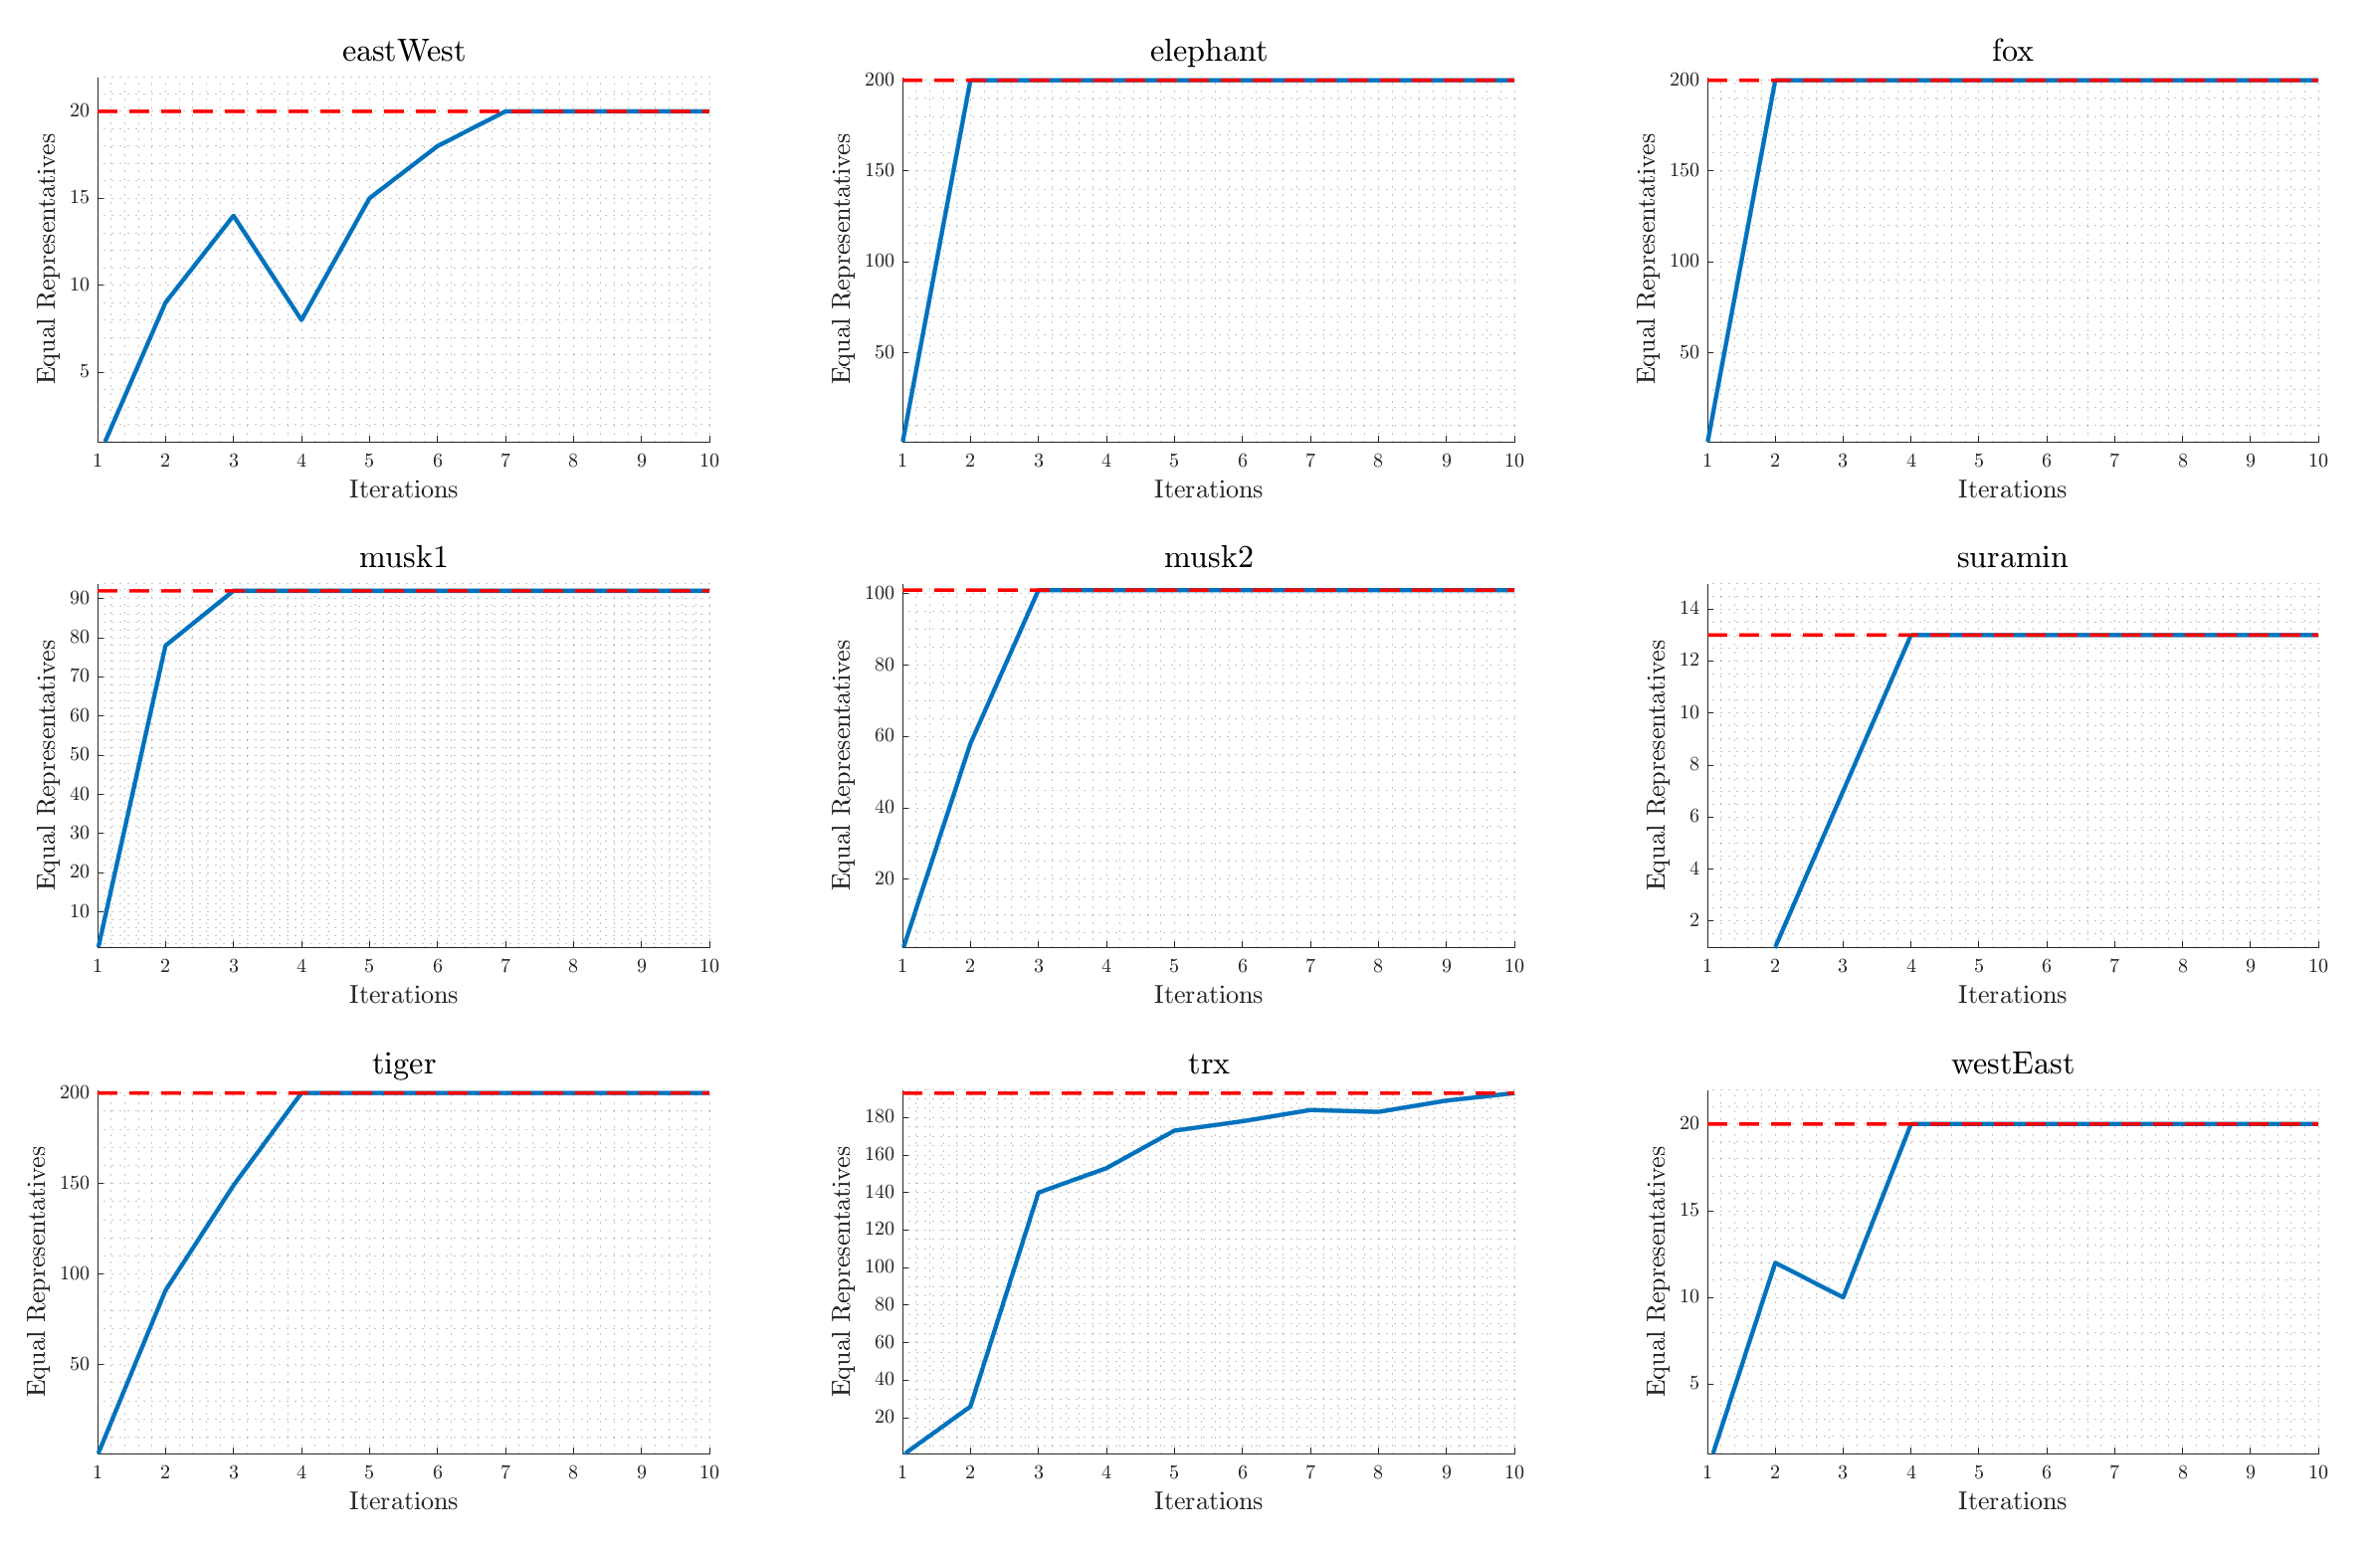
\includegraphics[width=0.94\textwidth]{figures/convergence.png} 
\caption{Bag representative convergence plots on 9 datasets. The blue line shows the number of bag representatives that are equal from one iteration to the next. The red dashed line represents the total number of bags.}\label{fig:convegence}
\end{figure}

\begin{figure}[t!]
    \centering
    \begin{minipage}{0.5\textwidth}
        \centering
        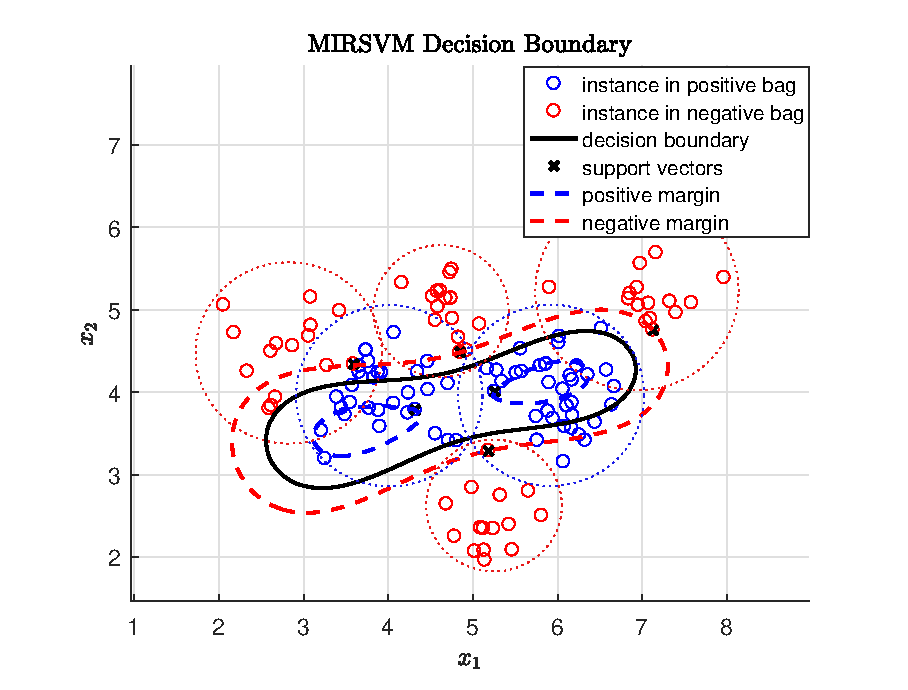
\includegraphics[width=\textwidth]{figures/mirsvm_figure.eps} % first figure itself
    \end{minipage}\hfill
    \begin{minipage}{0.5\textwidth}
        \centering
        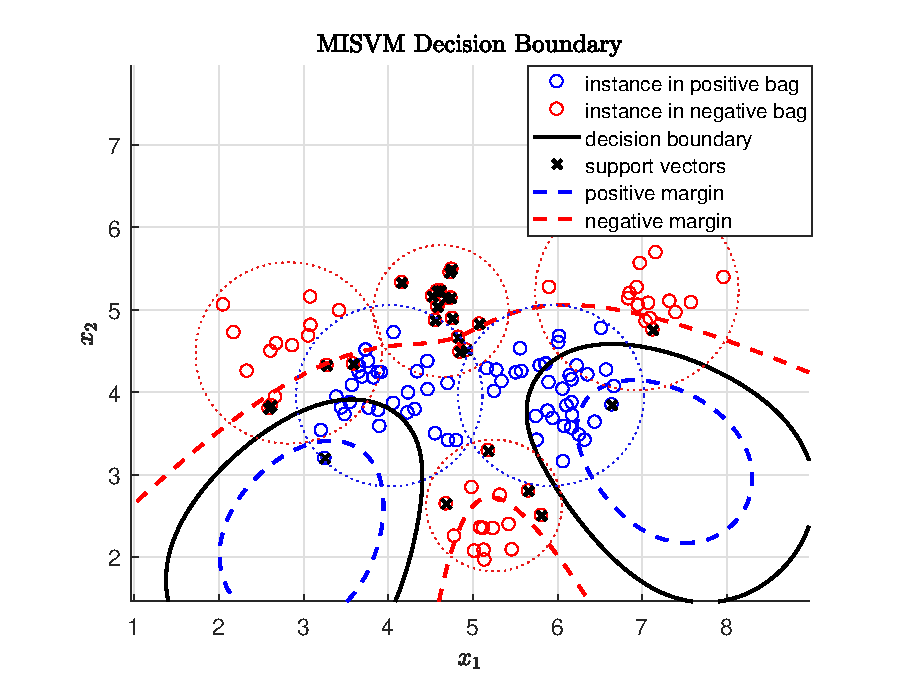
\includegraphics[width=\textwidth]{figures/misvm_figure.eps} % second figure itself
    \end{minipage}
    \caption{Difference between MIRSVM and MISVM on a random $2$-dimensional toy dataset. Note the differing number of support vectors produced by the two methods. MIRSVM has $6$, one for each bag, and MISVM has $29$. Also note the smoother representation of the data distribution given by MIRSVM's decision boundary, unlike MISVM whose decision boundary was greatly influenced by the larger number of support vectors belonging to the negative class with respect to the only $2$ positive support vectors.}\label{fig:diff}
\end{figure}
This formulation is designed to utilize and select representatives from positive and negative bags, unlike MISVM, which only optimizes over representatives from positive bags, while flattening the negative bag instances. MISVM allows multiple representatives to be chosen from negative bags and limits positive bag-representatives to be one, while MIRSVM allows for balanced bag-representative selection, where each bag is allowed one. MISVM also uses a wrapper method to initialize the positive bag-representatives by taking the mean vector of the instances within each positive bag. This is an implicit assumption that the instances within the positive bags are all positive, whereas MIRSVM's initialization procedure selects an instance from all bags at random, ensuring no noise is added by any wrapper techniques during initialization and no assumptions are made about the instances. Due to the constraints on the representatives, MIRSVM produces sparser models while MISVM has the freedom to select as many negative support vectors as it needs and restricts the support vectors chosen from positive bags to be one. Figure~\ref{fig:diff} shows the decision boundaries produced by MIRSVM and MISVM to highlight the differences in their solutions. As Figure~\ref{fig:diff} shows, MISVM produces a larger number of support vectors from the negative bags, which greatly influences the final decision boundary in favor of the negative class.

\section{Experimental Environment}
This section presents the experimental setup and comparison of our contribution, as well as $11$ other widely used methods on $15$ different benchmark datasets. The main aim of the experiments is to compare our contribution to other multi-instance support vector machines, contemporary multi-instance learners, and ensemble methods. 

Table~\ref{tab:Dataset} presents a summary of the $15$ datasets used throughout the experiments, where the number of attributes, bags, and total number of instances are shown. The datasets were obtained from the Weka\footnote{http://www.cs.waikato.ac.nz/ml/weka}~\cite{Hall2009} and KEEL\footnote{http://sci2s.ugr.es/keel/datasets.php}~\cite{Alca2011} dataset repositories. 

\begin{table}[t!]
\centering
\caption{Multi-Instance (MI) Classification datasets}
\small
\label{tab:Dataset}
\resizebox{0.95\textwidth}{!}{\begin{tabular}{l@{\extracolsep{\fill}}rrrrrr}
\hline\noalign{\smallskip}
Dataset & Attributes & Positive Bags & Negative Bags & Total & Instances & Avg. Bag Size\\
\noalign{\smallskip}\hline\noalign{\smallskip}
Suramin & 20 & 7 & 6 & 13 & 2898 &  222.92 \\ 
EastWest & 24 & 10 & 10 & 20 & 213 &  10.65  \\ 
WestEast & 24 & 10 & 10 & 20 & 213 &  10.65  \\ 
Musk1 & 166 & 47 & 45 & 92 & 476 &  5.17  \\ 
Musk2 & 166 & 39 & 62 & 101 & 6728 &  66.61  \\ 
Webmining & 5863 & 21 & 92 & 113 & 3423 &  30.29  \\ 
Mutagenesis-atoms & 10 & 125 & 63 & 188 & 1618 &  8.61  \\ 
Mutagenesis-bonds & 16 & 125 & 63 & 188 & 4081 &  21.71  \\ 
Mutagenesis-chains & 24 & 125 & 63 & 188 & 5424 &  28.85  \\ 
TRX & 8 & 25 & 168 & 193 & 26611 &  137.88 \\ 
Elephant & 230 & 100 & 100 & 200 & 1391 &  6.96 \\ 
Fox & 230 & 100 & 100 & 200 & 1320 &  6.60 \\ 
Tiger & 230 & 100 & 100 & 200 & 1188 &  5.94  \\ 
Component & 200 & 423 & 2707 & 3130 & 36894 &  11.79  \\ 
Function & 200 & 443 & 4799 & 5242 & 55536 &  10.59  \\ 
\noalign{\smallskip}\hline
\end{tabular}}
\end{table}

The experimental environment was designed to test the difference in performance of the proposed method against $11$ competing algorithms, contrasting instance-level, bag-level, and ensemble methods. Instance-level methods include MIOptimalBall, MIBoost, MISVM, MIDD, and MIWrapper. Bag-level methods include MISMO, SimpleMI, miGraph, and TLC. The ensemble-based bag-space methods, Bagging and Stacking, were also used. The base algorithms selected for the ensembles Bagging and Stacking were TLC, and TLC and SimpleMI, respectively. These algorithms were chosen because they have shown considerable performance in learning multi-instance models, while also having their frameworks readily available for reproducing their results through MILK, the Multi-Instance Learning Kit\footnote{http://www.cs.waikato.ac.nz/ml/milk}~\cite{Xu2003}, used in conjunction with the Weka framework. Experiments were run on an Intel i7-6700k CPU with 32GB RAM. MIRSVM was implemented in MATLAB while the referenced algorithms are available in the Java implementation of Weka with the exception of miGraph which was made available by Zhou et al.\footnote{http://lamda.nju.edu.cn/code\_miGraph.ashx} and tested in MATLAB.

We have compared the models trained on the different hyper-parameters using the cross-validation (CV) procedure which ensures that the models’ performances are accurately assessed and the model built is not biased towards the full dataset. The tuning of the model includes finding the best penalty parameter, $C$, as well as the best shape parameter for the Gaussian radial basis function kernel, $\sigma$. The best hyper-parameters were chosen from the following $6 \times 6$ possible combination runs, shown in Equations~\eqref{eq:paramC} and~\eqref{eq:miparamG}, referred to as~\eqref{eq:hyperparam}. 
\begin{subequations}
\label{eq:hyperparam}
\begin{align}
C \in  & \{0.1, 1, 10, 100, 1000, 10000\} \label{eq:paramC}\\
\sigma \in  & \{0.1, 0.5, 1, 2, 5, 10\} \label{eq:miparamG}
\end{align}
\end{subequations}
These parameters were also used for the compared SVM methods. This was done in order to keep the experimental environment controlled and ensure fair evaluation of the multi-instance SVM algorithms. The parameters for the referenced algorithms used throughout the experiments were those specified by their authors.

\section{Results \& Statistical Analysis}
The classification performance was measured using five metrics: Accuracy~\eqref{eq:accuracy}, Precision \eqref{eq:precision}, Recall~\eqref{eq:recall}, Cohen's kappa rate~\eqref{eq:kappa}, and Area under ROC curve (AUC)~\eqref{eq:auc}. The Precision and Recall measures were reported because Accuracy alone can be misleading when classes are imbalanced, as is the case with the \textit{component} and \textit{function} datasets, which respectively have six and ten times as many negative bags than positive. Cohen's Kappa Rate and the AUC measures are used as complementary measures in order to evaluate the algorithms comprehensively. Cohen's kappa rate, shown in Equation~\eqref{eq:kappa}, evaluates classifier merit according to the class distribution and ranges between -1 (full disagreement), 0 (random classification), and 1 (full agreement). The AUC metric highlights the trade-off between the true positive rate, or recall, and the false positive rate, as shown in Equation~\eqref{eq:auc}. The values of the true positive (TP), true negative (TN), false positive (FP), and false negative samples (FN) were first collected for each of the classifiers, then the metrics were computed using the equations shown in~\eqref{eq:metrics} on the $n^\prime$ bags of the test data, where $n^\prime = TP + FP + TN + FN$. The run times (training and testing times) of each algorithm are also reported to analyze the scalability and speed of each of the algorithms across differently sized datasets. 

The results for the following are shown in Tables~\ref{tab:accResults},~\ref{tab:preResults},~\ref{tab:recResults},~\ref{tab:kappaResults},~\ref{tab:aucResults}, and~\ref{tab:time}.
\begin{subequations}
\label{eq:metrics}
\begin{align}
\text{Accuracy} \tab \tab &\dfrac{TP+TN}{n^\prime} \label{eq:accuracy}\\[10pt]
\text{Precision} \tab \tab &\dfrac{TP}{TP+FP} \label{eq:precision}\\[10pt]
\text{Recall} \tab \tab &\dfrac{TP}{TP+FN} \label{eq:recall}\\[10pt]
\text{Cohen's Kappa Rate} \tab \tab &\dfrac{n^\prime - \dfrac{(TP+FN)*(TP+FP)}{n^\prime}}{1 - \dfrac{(TP+FN)*(TP+FP)}{n^\prime}} \label{eq:kappa}\\[10pt]
\text{Area Under ROC Curve} \tab \tab &\frac{1 + \dfrac{TP}{TP+FN} - \dfrac{FP}{FP+TN}}{2} \label{eq:auc}
\end{align}
\end{subequations}

In order to analyze the performances of the multiple models, non-parametric statistical tests are used to validate the experimental results obtained. The Iman-Davenport non-parametric test is run to investigate whether significant differences exist among the performance of the algorithms by ranking them over the datasets used, using the Friedman test. The algorithm ranks for each metric in Equations~\eqref{eq:metrics} are presented in the last row of the results tables, and the lowest (best) rank value is typeset in bold. Table~\ref{tab:metarank} contains the ranks and meta-rank of all methods, which helps determine and visualize the best performing algorithms across all datasets and metrics. 
\newpage
After the Iman-Davenport test indicates significant differences, the Bonferroni-Dunn post-hoc test~\cite{Dunn1961} is then used to find where they occur between algorithms by assuming the classifiers' performances are different by at least some critical value. Below each result table, a figure highlighting the critical distance (in gray), from the best ranking algorithm to the rest, is shown. The algorithms to the right of the critical distance bar perform statistically significantly worse than the control algorithm, MIRSVM. Figures \ref{fig:BonfDunnacc}, \ref{fig:BonfDunnprec}, \ref{fig:BonfDunnrec}, \ref{fig:BonfDunnkappa}, \ref{fig:BonfDunnauc}, \ref{fig:BonfDunnpmeta} show the results of the Bonferroni-Dunn post-hoc procedure over the metrics in~\eqref{eq:metrics}, as well as the meta-rank results in Table~\ref{tab:metarank}. The Holm (multiple) and Wilcoxon (pairwise) rank-sum post-hoc tests~\cite{Holander1999} were then run for each of the metrics to compute multiple and pairwise comparisons between the proposed algorithm and the other methods compared, investigating whether statistical differences exist among the algorithms' results. Tables~\ref{tab:MIstatacc},~\ref{tab:statprec},~\ref{tab:statrec},~\ref{tab:statkappa}, and~\ref{tab:statauc} show the $p$-values for the Holm test for $\alpha = 0.05$, and the rank-sums and adjusted $p$-values for the Wilcoxon test.

\subsection{Accuracy}
The results for accuracy indicate that the bag-based and ensemble learners perform better than the instance-based and wrapper methods. MIRSVM achieves the best accuracy over $5$ of the $15$ datasets with a competitive average against miGraph, Bagging, Stacking, and TLC. Note that MIRSVM performs better than MISVM for all datasets, indicating that using representatives from each bag and limiting the number of support vectors per negative bag improves the classification performance. The instance-level classifiers and wrapper methods, such as MIBoost, MIWrapper, and SimpleMI perform the worst. This behavior emphasizes the importance of not making prior assumptions about the positive bags' distributions. 

Figure~\ref{fig:BonfDunnacc} and Table~\ref{tab:statacc} show the results for the statistical analysis on the accuracy results. The algorithms with ranking higher than $5.63$ (MIRSVM rank + Bonferroni-Dunn critical value), to the right of the grey bar in Figure~\ref{fig:BonfDunnacc}, perform statistically worse than MIRSVM. Table~\ref{tab:statacc} shows the $p$-values of the Holm and Wilcoxon tests and their results complement one another. Holm's procedure rejects those hypotheses having a $p$-value $\leq 0.01$, thus indicating that MIRSVM performs significantly better than all methods except miGraph, Bagging, Stacking, and TLC. The Wilcoxon $p$-values show significant differences exist among all algorithms except miGraph, Bagging, and Stacking. They also show that MIRSVM has significantly better accuracy than MIBoost, MIOptimalBall, MIDD, MIWrapper, MISMO, MISVM, and SimpleMI, each having respectively small $p$-values, highlighting MIRSVM's superior classification accuracy. 
\begin{table}[t!]
\caption{Accuracy for MI classifiers}\label{tab:accResults}
\resizebox{0.95\textwidth}{!}{\begin{tabular}{l@{\extracolsep{\fill}}ccccccccccccc}
\noalign{\smallskip}\hline\noalign{\smallskip}
Datasets &MIRSVM & miGraph & MIBoost &MIOptimalBall &MIDD &MIWrapper &MISMO &MISVM &SimpleMI &TLC &Bagging &Stacking \\
\noalign{\smallskip}\hline\noalign{\smallskip}
suramin &0.8000 &\textbf{0.8462} &0.5000 &0.7250 &0.4250 &0.5000 &0.7250 &0.5000 &0.5000 &0.6000 &0.6650 &0.4615 &  \\
eastWest &\textbf{0.8000} &0.7000 &0.5000 &0.7250 &0.6125 &0.5000 &0.7125 &0.5625 &0.5000 &0.6000 &0.6000 &0.4500 &  \\
westEast &0.7500 &0.7500 &0.5000 &0.3750 &0.4500 &0.5000 &0.7375 &0.4125 &0.5000 &0.5625 &\textbf{0.9649} &0.6375 &  \\
musk1 &\textbf{0.9022} &0.8152 &0.5109 &0.7717 &0.8804 &0.5109 &0.7826 &0.7609 &0.5109 &0.8587 &0.8142 &0.8587 &  \\
musk2 &0.8218 &0.7426 &0.6139 &0.7723 &0.7228 &0.6139 &0.7030 &0.7129 &0.6139 &0.6238 &\textbf{0.8756} &0.6733 &  \\
webmining &0.8500 &0.8142 &0.8142 &0.7699 &0.8142 &0.8142 &0.8407 &0.6903 &0.8142 &0.8142 &\textbf{0.9358} &0.8053 &  \\
trx &0.8860 &0.8964 &0.8705 &\textbf{0.9016} &0.8808 &0.8705 &0.8705 &0.8705 &0.8705 &0.8756 &0.6450 &0.8860 &  \\
mutagenesis-atoms &0.7714 &0.7606 &0.6649 &0.6436 &0.7074 &0.6649 &0.6915 &0.6649 &0.6649 &\textbf{0.7766} &\textbf{0.7766} &0.7606 &  \\
mutagenesis-bonds &0.8252 &0.7872 &0.6649 &0.6915 &0.7713 &0.6649 &0.7979 &0.6649 &0.6649 &0.8351 &0.8351 &\textbf{0.8564} &  \\
mutagenesis-chains &\textbf{0.8411} &0.7926 &0.6649 &0.6702 &0.7766 &0.6649 &0.8351 &0.6649 &0.6649 &0.8404 &0.8404 &0.8351 &  \\
tiger &0.7750 &0.7950 &0.5000 &0.5000 &0.7100 &0.5000 &0.7200 &0.7550 &0.5000 &0.6650 &\textbf{0.8000} &0.7250 &  \\
elephant &\textbf{0.8300} &\textbf{0.8300} &0.5000 &0.5000 &0.7900 &0.5000 &0.8100 &0.8000 &0.5000 &0.8000 &0.5625 &0.8250 &  \\
fox &0.6550 &0.6300 &0.5000 &0.5000 &0.5800 &0.5000 &0.5250 &0.4750 &0.5000 &0.6450 &\textbf{0.8587} &0.6500 &  \\
component &\textbf{0.9366} &0.9153 &0.8649 &0.8696 &0.8780 &0.8649 &0.8968 &0.8703 &0.8649 &0.9358 &0.6000 &0.9355 &  \\
function &0.9523 &0.9405 &0.9155 &0.9138 &0.9193 &0.9155 &0.9376 &0.9195 &0.9155 &\textbf{0.9649} &0.6238 &0.9647 &  \\
\noalign{\smallskip}\hline\noalign{\smallskip}
Average &\textbf{0.8264} &0.8010 &0.6390 &0.6886 &0.7279 &0.6390 &0.7724 &0.6883 &0.6390 &0.7598 &0.7598 &0.7550 &  \\
Rank &\textbf{2.2000} &3.8667 &9.6000 &7.8667 &6.5667 &9.6000 &5.3333 &8.5667 &9.6000 &4.7000 &4.8667 &5.2333 &  \\
\noalign{\smallskip}\hline
\end{tabular}}
\centering
\resizebox{0.95\textwidth}{!}{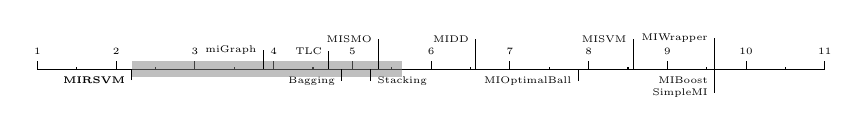
\begin{tikzpicture}
\draw (1,0) -- (11,0);
\foreach \x in {1,2,3,4,5,6,7,8,9,10,11} {
\draw (\x, 0) -- ++(0,.1) node [above,scale=0.7] {\tiny \x};
\ifthenelse{\x < 11}{\draw (\x+.5, 0) -- ++(0,.03);}{}
}

\coordinate (c0) at (2.2,0);
\coordinate (c1) at (3.8667,0);
\coordinate (c2) at (9.6,0);
\coordinate (c3) at (7.8667,0);
\coordinate (c4) at (6.5667,0);
\coordinate (c5) at (9.6,0);
\coordinate (c6) at (5.3333,0);
\coordinate (c7) at (8.5667,0);
\coordinate (c8) at (9.6,0);
\coordinate (c9) at (4.7,0);
\coordinate (c10) at (4.8667,0);
\coordinate (c11) at (5.2333,0);

\node (l0) at (c0) [below left=.01cm and 0cm, align=right,scale=0.7] {\tiny \textbf{MIRSVM}};
\node (l1) at (c1) [above left=.1cm and 0cm, align=right,scale=0.7] {\tiny miGraph};
\node (l2) at (c2) [below left=.01cm and 0cm, align=right,scale=0.7] {\tiny MIBoost};
\node (l3) at (c3) [below left=.01cm and 0cm, align=right,scale=0.7] {\tiny MIOptimalBall};
\node (l4) at (c4) [above left=.25cm and 0cm, align=right,scale=0.7] {\tiny MIDD};
\node (l5) at (c5) [above left=.25cm and 0cm, align=right,scale=0.7] {\tiny MIWrapper};
\node (l6) at (c6) [above left=.25cm and 0cm, align=right,scale=0.7] {\tiny MISMO};
\node (l7) at (c7) [above left=.25cm and 0cm, align=right,scale=0.7] {\tiny MISVM};
\node (l8) at (c8) [below left=.16cm and 0cm, align=right,scale=0.7] {\tiny SimpleMI};
\node (l9) at (c9) [above left=.1cm and 0cm, align=right,scale=0.7] {\tiny TLC};
\node (l10) at (c10) [below left=.01cm and 0cm, align=right,scale=0.7] {\tiny Bagging};
\node (l11) at (c11) [below right=.01cm and 0cm, align=left,scale=0.7] {\tiny Stacking};

\fill[fill=gray,fill opacity=0.5] (2.2,-0.1) rectangle (5.635,0.1);

\foreach \x in {0,1,2,3,4,5,6,7,8,9,10,11} {
\draw (l\x) -| (c\x);
};
\end{tikzpicture}}\vspace{-1.8em}
\captionof{figure}{Bonferroni-Dunn test for Accuracy}\label{fig:BonfDunnacc}\vspace{-1.3em}
\captionof{table}{Holm and Wilcoxon tests for Accuracy}\label{tab:MIstatacc}
\scriptsize
\resizebox{0.95\textwidth}{!}{\begin{tabular}{lccccccccccc}
\noalign{\smallskip}\hline\noalign{\smallskip}
MIRSVM vs. &miGraph &MIBoost &MIOptimalBall &MIDD &MIWrapper &MISMO &MISVM &SimpleMI &TLC &Bagging &Stacking \\
\noalign{\smallskip}\hline\noalign{\smallskip}
Holm $p$-value &0.0500 &0.0045 &0.0071 &0.0083 &0.0050 &0.0100 &0.0063 &0.0056 &0.0250 &0.0167 &0.0125 \\\noalign{\smallskip}\hline\noalign{\smallskip}
Wilcoxon $p$-value &0.0279 &0.0001 &0.0001 &0.0001 &0.0001 &0.0001 &0.0001 &0.0001 &0.0067 & 0.3028 &0.0103 \\
Wilcoxon R$^+$ &98.500 &120.00 &119.00 &120.00 &120.00 &120.00 &120.00 &120.00 &106.00 &79.000 &104.00 \\
Wilcoxon R$^-$ &21.500 & 0.0000 &1.0000 & 0.0000 &0.0000 &0.0000 &0.0000 &0.0000 &14.000 &41.000 &16.000 \\
\noalign{\smallskip}\hline\noalign{\smallskip}
\end{tabular}}
\end{table}

\subsection{Precision \& Recall}
Precision and recall are conflicting metrics that must be evaluated together in order to observe their behavior, since they are both used to measure relevance. The results for MIWrapper and SimpleMI indicate that they are unstable classifiers, exhibiting extreme variance in behavior, making them unsuitable for real-world applications. It is also interesting to analyze the performance on the mutagenesis datasets which have a larger number of positive bags than negative, where MISVM, MIBoost, MIWrapper, and SimpleMI predict all bags as negative. Additionally, while MISMO obtains unbiased results on these datasets, MIRSVM significantly outperforms it over both precision and recall, achieving a better trade-off.  
\begin{table}[H]
\caption{Precision for MI classifiers}\label{tab:preResults}
\resizebox{0.95\textwidth}{!}{\begin{tabular}{l@{\extracolsep{\fill}}ccccccccccccc}
\noalign{\smallskip}\hline\noalign{\smallskip}
Datasets &MIRSVM & miGraph & MIBoost &MIOptimalBall &MIDD &MIWrapper &MISMO &MISVM &SimpleMI &TLC &Bagging &Stacking \\
\noalign{\smallskip}\hline\noalign{\smallskip}
suramin &0.7778 &0.7778 &\textbf{1.0000} &\textbf{1.0000} &0.2857 &\textbf{1.0000} &\textbf{1.0000} &0.5000 &\textbf{1.0000} &0.6429 &0.6514 &0.4000 &  \\
eastWest &0.7143 &0.7000 &0.5000 &0.8750 &0.5882 &0.5000 &0.7429 &\textbf{1.0000} &0.5000 &0.6053 &0.6053 &0.4444 &  \\
westEast &0.7272 &0.7273 &0.5000 &0.2727 &0.4600 &0.5000 &0.6939 &0.3600 &0.5000 &0.5581 &\textbf{0.9729} &0.6038 &  \\
musk1 &0.8519 &0.7778 &\textbf{1.0000} &0.9286 &0.9048 &\textbf{1.0000} &0.8049 &0.8108 &\textbf{1.0000} &0.8478 &0.8817 &0.8478 &  \\
musk2 &0.7059 &0.7826 &0.6139 &0.7826 &0.7576 &0.6139 &0.7424 &0.7538 &0.6139 &0.7400 &\textbf{0.9138} &0.7164 &  \\
webmining &0.7500 &\textbf{1.0000} &0.8142 &0.8173 &0.8142 &0.8142 &0.8936 &\textbf{1.0000} &0.8142 &0.8817 &0.9462 &0.8500 &  \\
trx &\textbf{1.0000} &0.8571 &0.8705 &0.9306 &0.9191 &0.8705 &0.8705 &0.8705 &0.8705 &0.9138 &0.6747 &0.9011 &  \\
mutagenesis-atoms &0.7872 &0.7985 &\textbf{1.0000} &0.4630 &0.6111 &\textbf{1.0000} &0.5439 &\textbf{1.0000} &\textbf{1.0000} &0.7059 &0.7059 &0.6667 &  \\
mutagenesis-bonds &0.8468 &0.8195 &\textbf{1.0000} &0.5385 &0.7500 &\textbf{1.0000} &0.6812 &\textbf{1.0000} &\textbf{1.0000} &0.7857 &0.7857 &0.8333 &  \\
mutagenesis-chains &0.8571 &0.8116 &\textbf{1.0000} &0.5091 &0.7059 &\textbf{1.0000} &0.7759 &\textbf{1.0000} &\textbf{1.0000} &0.7705 &0.7705 &0.7581 &  \\
tiger &0.7365 &0.7323 &0.5000 &0.5000 &0.6944 &0.5000 &0.7444 &0.7802 &0.5000 &0.6514 &\textbf{0.8000} &0.7320 &  \\
elephant &0.8576 &\textbf{0.8750} &0.5000 &0.5000 &0.7959 &0.5000 &0.8444 &0.7679 &0.5000 &0.8000 &0.5581 &0.8283 &  \\
fox &0.6040 &0.6275 &0.5000 &0.5000 &0.5833 &0.5000 &0.5287 &0.4854 &0.5000 &0.6747 &\textbf{0.8478} &0.6705 &  \\
component &\textbf{0.9866} &0.7782 &0.8649 &0.8778 &0.8902 &0.8649 &0.8958 &0.8696 &0.8649 &0.9462 &0.6429 &0.9449 &  \\
function &0.8459 &0.6775 &0.9155 &0.9202 &0.9317 &0.9155 &0.9376 &0.9197 &0.9155 &\textbf{0.9729} &0.7400 &0.9726 &  \\
\noalign{\smallskip}\hline\noalign{\smallskip}
Average &0.8033 &0.7828 &0.7719 &0.6944 &0.7128 &0.7719 &0.7800 &\textbf{0.8079} &0.7719 &0.7665 &0.7665 &0.7447 &  \\
Rank &\textbf{5.3333} &6.1333 &7.1000 &7.3333 &7.3667 &7.1000 &5.8667 &5.8667 &7.1000 &5.9000 &6.3333 &6.5667 &  \\
\noalign{\smallskip}\hline
\end{tabular}}
\centering
\resizebox{0.95\textwidth}{!}{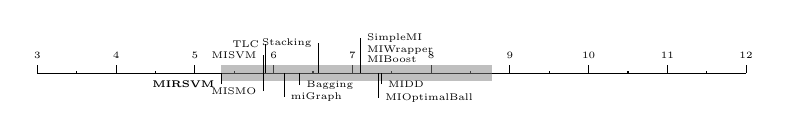
\begin{tikzpicture}
\draw (3,0) -- (12,0);
\foreach \x in {3,4,5,6,7,8,9,10,11,12} {
\draw (\x, 0) -- ++(0,.1) node [above,scale=0.7] {\tiny \x};
\ifthenelse{\x < 12}{\draw (\x+.5, 0) -- ++(0,.03);}{}
}

\coordinate (c0) at (5.3333,0);
\coordinate (c1) at (6.1333,0);
\coordinate (c2) at (7.1,0);
\coordinate (c3) at (7.3333,0);
\coordinate (c4) at (7.3667,0);
\coordinate (c5) at (7.1,0);
\coordinate (c6) at (5.8667,0);
\coordinate (c7) at (5.8667,0);
\coordinate (c8) at (7.1,0);
\coordinate (c9) at (5.9,0);
\coordinate (c10) at (6.3333,0);
\coordinate (c11) at (6.5667,0);

\node (l0) at (c0) [below left=.01cm and 0cm, align=right,scale=0.7] {\tiny \textbf{MIRSVM}};
\node (l1) at (c1) [below right=.16cm and 0cm, align=left,scale=0.7] {\tiny miGraph};
\node (l2) at (c2) [above right=.05cm and 0cm, align=left,scale=0.7] {\tiny MIBoost};
\node (l3) at (c3) [below right=.17cm and 0cm, align=left,scale=0.7] {\tiny MIOptimalBall};
\node (l4) at (c4) [below right=.01cm and 0cm, align=left,scale=0.7] {\tiny MIDD};
\node (l5) at (c5) [above right=.15cm and 0cm, align=left,scale=0.7] {\tiny MIWrapper};
\node (l6) at (c6) [below left=.1cm and 0cm, align=right,scale=0.7] {\tiny MISMO};
\node (l7) at (c7) [above left=.1cm and 0cm, align=right,scale=0.7] {\tiny MISVM};
\node (l8) at (c8) [above right=.3cm and 0cm, align=left,scale=0.7] {\tiny SimpleMI};
\node (l9) at (c9) [above left=.24cm and 0cm, align=right,scale=0.7] {\tiny TLC};
\node (l10) at (c10) [below right=.01cm and 0cm, align=left,scale=0.7] {\tiny Bagging};
\node (l11) at (c11) [above left=.24cm and 0cm, align=right,scale=0.7] {\tiny Stacking};

\fill[fill=gray,fill opacity=0.5] (5.3333,-0.1) rectangle (8.7683,0.1);

\foreach \x in {0,1,2,3,4,5,6,7,8,9,10,11} {
\draw (l\x) -| (c\x);};
\end{tikzpicture}}\vspace{-1.8em}
\captionof{figure}{Bonferroni-Dunn test for Precision}\label{fig:BonfDunnprec}\vspace{-1.3em}
\captionof{table}{Holm and Wilcoxon tests for Precision}\label{tab:statprec}
\scriptsize
\resizebox{0.95\textwidth}{!}{\begin{tabular}{lccccccccccc}
\noalign{\smallskip}\hline\noalign{\smallskip}
MIRSVM vs. &miGraph &MIBoost &MIOptimalBall &MIDD &MIWrapper &MISMO &MISVM &SimpleMI &TLC &Bagging &Stacking \\
\noalign{\smallskip}\hline\noalign{\smallskip}
Holm $p$-value &0.0125 &0.0056 &0.0050 &0.0045 &0.0063 &0.0250 &0.0500 &0.0071 &0.0167 &0.0100 &0.0083 \\\noalign{\smallskip}\hline\noalign{\smallskip}
Wilcoxon $p$-value & 0.4212 & 0.5614 &0.0946 &0.0256 & 0.5614 & 0.4212 & 0.8039 & 0.5614 &0.1354 & 0.4543 &0.1354 \\
Wilcoxon R$^+$ &75.000 &71.000 &90.000 &99.000 &71.000 &75.000 &55.000 &71.000 &87.000 &74.000 &87.000 \\
Wilcoxon R$^-$ &45.000 &49.000 &30.000 &21.000 &49.000 &45.000 &65.000 &49.000 &33.000 &46.000 &33.000 \\
\noalign{\smallskip}\hline\noalign{\smallskip}
\end{tabular}}
\end{table}
Figure~\ref{fig:BonfDunnprec} and~\ref{fig:BonfDunnrec} show that there are no significant differences between the precision and recall results obtained by all algorithms. Note, MIRSVM outperforms both ensemble methods according to recall, despite them exhibiting good accuracy and precision, indicating they are strongly conservative towards predicting positive bags. Holm's test indicates significant differences exist between MIRSVM and all algorithms except miGraph, MISMO, MISVM, and TLC for precision, and all the above along with SimpleMI, MIOptimalBall, and Bagging for recall. The Wilcoxon test does not reflect significant differences for precision, does for recall. The tests are severely biased due to the classifier's extreme unbalanced behavior, whereas MIRSVM demonstrates proper balance of the precision-recall trade-off.
\begin{table}[t!]
\caption{Recall for MI classifiers}\label{tab:recResults}
\resizebox{0.95\textwidth}{!}{\begin{tabular}{l@{\extracolsep{\fill}}ccccccccccccc}
\noalign{\smallskip}\hline\noalign{\smallskip}
Datasets &MIRSVM & miGraph & MIBoost &MIOptimalBall &MIDD &MIWrapper &MISMO &MISVM &SimpleMI &TLC &Bagging &Stacking \\
\noalign{\smallskip}\hline\noalign{\smallskip}
suramin &\textbf{1.0000} &\textbf{1.0000} &0.0000 &0.4500 &0.1000 &0.0000 &0.4500 &0.5000 &0.0000 &0.4500 &0.7100 &0.3333 &  \\
eastWest &\textbf{1.0000} &0.7000 &0.7000 &0.5250 &0.7500 &0.7000 &0.6500 &0.1250 &\textbf{1.0000} &0.5750 &0.5750 &0.4000 &  \\
westEast &0.8000 &0.8000 &0.9000 &0.1500 &0.5750 &0.9000 &0.8500 &0.2250 &\textbf{1.0000} &0.6000 &0.9892 &0.8000 &  \\
musk1 &\textbf{0.9787} &0.8936 &0.0000 &0.5778 &0.8444 &0.0000 &0.7333 &0.6667 &0.0000 &0.8667 &0.8913 &0.8667 &  \\
musk2 &0.9231 &0.4615 &\textbf{1.0000} &0.8710 &0.8065 &\textbf{1.0000} &0.7903 &0.7903 &\textbf{1.0000} &0.5968 &0.9464 &0.7742 &  \\
webmining &0.2857 &0.0000 &\textbf{1.0000} &0.9239 &\textbf{1.0000} &\textbf{1.0000} &0.9130 &0.6196 &\textbf{1.0000} &0.8913 &0.9815 &0.9239 &  \\
trx &0.4833 &0.2400 &\textbf{1.0000} &0.9583 &0.9464 &\textbf{1.0000} &\textbf{1.0000} &\textbf{1.0000} &\textbf{1.0000} &0.9464 &0.5600 &0.9762 &  \\
mutagenesis-atoms &\textbf{0.8880} &0.8560 &0.0000 &0.3968 &0.3492 &0.0000 &0.4921 &0.0000 &0.0000 &0.5714 &0.5714 &0.5714 &  \\
mutagenesis-bonds &\textbf{0.8960} &0.8720 &0.0000 &0.5556 &0.4762 &0.0000 &0.7460 &0.0000 &0.0000 &0.6984 &0.6984 &0.7143 &  \\
mutagenesis-chains &\textbf{0.9120} &0.8960 &0.0000 &0.4444 &0.5714 &0.0000 &0.7143 &0.0000 &0.0000 &0.7460 &0.7460 &0.7460 &  \\
tiger &0.8700 &0.9300 &0.5000 &\textbf{1.0000} &0.7500 &0.5000 &0.6700 &0.7100 &\textbf{1.0000} &0.7100 &0.8000 &0.7100 &  \\
elephant &0.9100 &0.7700 &0.6000 &\textbf{1.0000} &0.7800 &0.6000 &0.7600 &0.8600 &\textbf{1.0000} &0.8000 &0.6000 &0.8200 &  \\
fox &0.9000 &0.6400 &0.7000 &\textbf{1.0000} &0.5600 &0.7000 &0.4600 &0.8300 &\textbf{1.0000} &0.5600 &0.8667 &0.5900 &  \\
component &0.5839 &0.5225 &\textbf{1.0000} &0.9867 &0.9797 &\textbf{1.0000} &0.9967 &\textbf{1.0000} &\textbf{1.0000} &0.9815 &0.4500 &0.9826 &  \\
function &0.5327 &0.5643 &\textbf{1.0000} &0.9919 &0.9840 &\textbf{1.0000} &0.9983 &0.9994 &\textbf{1.0000} &0.9892 &0.5968 &0.9894 &  \\
\noalign{\smallskip}\hline\noalign{\smallskip}
Average &\textbf{0.7976} &0.6764 &0.5600 &0.7221 &0.6982 &0.5600 &0.7483 &0.5551 &0.6667 &0.7322 &0.7322 &0.7465 &  \\
Rank &4.8667 &6.5667 &6.8667 &6.3333 &7.3667 &6.8667 &6.7000 &7.4333 &\textbf{4.8333} &7.3667 &6.0667 &6.7333 &  \\
\noalign{\smallskip}\hline
\end{tabular}}
\resizebox{0.95\textwidth}{!}{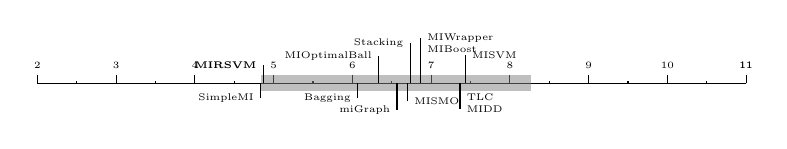
\begin{tikzpicture}
\draw (2,0) -- (11,0);
\foreach \x in {2,3,4,5,6,7,8,9,10,11,11} {
\draw (\x, 0) -- ++(0,.1) node [above,scale=0.7] {\tiny \x};
\ifthenelse{\x < 11}{\draw (\x+.5, 0) -- ++(0,.03);}{}
}

\coordinate (c0) at (4.8667,0);
\coordinate (c1) at (6.5667,0);
\coordinate (c2) at (6.8667,0);
\coordinate (c3) at (6.3333,0);
\coordinate (c4) at (7.3667,0);
\coordinate (c5) at (6.8667,0);
\coordinate (c6) at (6.7,0);
\coordinate (c7) at (7.4333,0);
\coordinate (c8) at (4.8333,0);
\coordinate (c9) at (7.3667,0);
\coordinate (c10) at (6.0667,0);
\coordinate (c11) at (6.7333,0);

\node (l0) at (c0) [above left=.1cm and 0cm, align=right,scale=0.7] {\tiny \textbf{MIRSVM}};
\node (l1) at (c1) [below left=.2cm and 0cm, align=right,scale=0.7] {\tiny miGraph};
\node (l2) at (c2) [above right=.3cm and 0cm, align=left,scale=0.7] {\tiny MIBoost};
\node (l3) at (c3) [above left=.2cm and 0cm, align=right,scale=0.7] {\tiny MIOptimalBall};
\node (l4) at (c4) [below right=.2cm and 0cm, align=left,scale=0.7] {\tiny MIDD};
\node (l5) at (c5) [above right=.43cm and 0cm, align=left,scale=0.7] {\tiny MIWrapper};
\node (l6) at (c6) [below right=.1cm and 0cm, align=left,scale=0.7] {\tiny MISMO};
\node (l7) at (c7) [above right=.23cm and 0cm, align=left,scale=0.7] {\tiny MISVM};
\node (l8) at (c8) [below left=.05cm and 0cm, align=right,scale=0.7] {\tiny SimpleMI};
\node (l9) at (c9) [below right=.05cm and 0cm, align=left,scale=0.7] {\tiny TLC};
\node (l10) at (c10) [below left=.05cm and 0cm, align=right,scale=0.7] {\tiny Bagging};
\node (l11) at (c11) [above left=.37cm and 0cm, align=right,scale=0.7] {\tiny Stacking};

\fill[fill=gray,fill opacity=0.5] (4.8333,-0.1) rectangle (8.2683,0.1);

\foreach \x in {0,1,2,3,4,5,6,7,8,9,10,11} {
\draw (l\x) -| (c\x);};
\end{tikzpicture}}\vspace{-1.8em}
\captionof{figure}{Bonferroni-Dunn test for Recall}\label{fig:BonfDunnrec}\vspace{-1.3em}
\captionof{table}{Holm and Wilcoxon tests for Recall}\label{tab:statrec}
\scriptsize
\resizebox{0.95\textwidth}{!}{\begin{tabular}{lccccccccccc}
\noalign{\smallskip}\hline\noalign{\smallskip}
MIRSVM vs. &miGraph &MIBoost &MIOptimalBall &MIDD &MIWrapper &MISMO &MISVM &SimpleMI &TLC &Bagging &Stacking \\
\noalign{\smallskip}\hline\noalign{\smallskip}
Holm $p$-value &0.0125 &0.0063 &0.0167 &0.0050 &0.0071 &0.0100 &0.0045 &0.0500 &0.0056 &0.0250 &0.0083 \\\noalign{\smallskip}\hline\noalign{\smallskip}
Wilcoxon $p$-value &0.0060 & 0.2077 & 0.5614 & 0.4543 & 0.2077 & 0.6387 &0.1070 & 0.6603 & 0.5995 &0.1354 & 0.5721 \\
Wilcoxon R$^+$ &106.50 &83.000 &71.000 &74.000 &83.000 &69.000 &89.000 &60.000 &70.000 &87.000 &62.000 \\
Wilcoxon R$^-$ &13.500 &37.000 &49.000 &46.000 &37.000 &51.000 &31.000 &45.000 &50.000 &33.000 &43.000 \\
\noalign{\smallskip}\hline\noalign{\smallskip}
\end{tabular}}
\end{table}

\subsection{Cohen's Kappa Rate}
\begin{table}[t!]
\caption{Cohen's Kappa Rate for MI classifiers}\label{tab:kappaResults}
\resizebox{0.95\textwidth}{!}{\begin{tabular}{lccccccccccccc}
\noalign{\smallskip}\hline\noalign{\smallskip}
Datasets &MIRSVM & miGraph & MIBoost &MIOptimalBall &MIDD &MIWrapper &MISMO &MISVM &SimpleMI &TLC &Bagging &Stacking \\
\noalign{\smallskip}\hline\noalign{\smallskip}
suramin &\textbf{0.6829} &\textbf{0.6829} &0.0000 &0.4500 &-0.1500 &0.0000 &0.4500 &0.0000 &0.0000 &0.2000 &0.3300 &-0.0964 &  \\
eastWest &\textbf{0.6000} &0.4000 &0.0000 &0.4500 &0.2250 &0.0000 &0.4250 &0.1250 &0.0000 &0.2000 &0.2000 &-0.1000 &  \\
westEast &0.5000 &0.5000 &0.0000 &-0.2500 &-0.1000 &0.0000 &0.4750 &-0.1750 &0.0000 &0.1250 &\textbf{0.7529} &0.2750 &  \\
musk1 &\textbf{0.8036} &0.6290 &0.0000 &0.5396 &0.7604 &0.0000 &0.5642 &0.5197 &0.0000 &0.7174 &0.3744 &0.7174 &  \\
musk2 &\textbf{0.6540} &0.4123 &0.0000 &0.5031 &0.4039 &0.0000 &0.3613 &0.3856 &0.0000 &0.2492 &0.3858 &0.2940 &  \\
webmining &0.3468 &0.0000 &0.0000 &0.0246 &0.0000 &0.0000 &0.4535 &0.3771 &0.0000 &0.3744 &\textbf{0.6945} &0.2458 &  \\
trx &0.2100 &0.3375 &0.0000 &\textbf{0.5228} &0.4224 &0.0000 &0.0000 &0.0000 &0.0000 &0.3858 &0.2900 &0.3364 &  \\
mutagenesis-atoms &\textbf{0.5395} &0.4431 &0.0000 &0.1709 &0.2654 &0.0000 &0.2909 &0.0000 &0.0000 &0.4738 &0.4738 &0.4431 &  \\
mutagenesis-bonds &0.5699 &0.5070 &0.0000 &0.3131 &0.4356 &0.0000 &0.5569 &0.0000 &0.0000 &0.6195 &0.6195 &\textbf{0.6659} &  \\
mutagenesis-chains &0.6303 &0.5094 &0.0000 &0.2359 &0.4738 &0.0000 &0.6225 &0.0000 &0.0000 &\textbf{0.6391} &\textbf{0.6391} &0.6285 &  \\
tiger &0.5500 &0.5900 &0.0000 &0.0000 &0.4200 &0.0000 &0.4400 &0.5100 &0.0000 &0.3300 &\textbf{0.6000} &0.4500 &  \\
elephant &\textbf{0.7000} &0.6600 &0.0000 &0.0000 &0.5800 &0.0000 &0.6200 &0.6000 &0.0000 &0.6000 &0.1250 &0.6500 &  \\
fox &0.3100 &0.2600 &0.0000 &0.0000 &0.1600 &0.0000 &0.0500 &-0.0500 &0.0000 &0.2900 &\textbf{0.7174} &0.3000 &  \\
component &0.6644 &0.5795 &0.0000 &0.1613 &0.2836 &0.0000 &0.3656 &0.0675 &0.0000 &\textbf{0.6945} &0.2000 &0.6906 &  \\
function &0.6292 &0.5838 &0.0000 &0.0966 &0.2801 &0.0000 &0.4083 &0.0933 &0.0000 &\textbf{0.7529} &0.2492 &0.7507 &  \\
\noalign{\smallskip}\hline\noalign{\smallskip}
Average &\textbf{0.5594} &0.4730 &0.0000 &0.2145 &0.2973 &0.0000 &0.4056 &0.1635 &0.0000 &0.4434 &0.4434 &0.4167 &  \\
Rank &\textbf{2.6333} &4.2000 &10.1667 &7.0000 &6.5333 &10.1667 &5.2333 &8.3667 &10.1667 &4.2667 &4.2667 &5.0000 &  \\
\noalign{\smallskip}\hline\noalign{\smallskip}
\end{tabular}}
\centering
\resizebox{0.95\textwidth}{!}{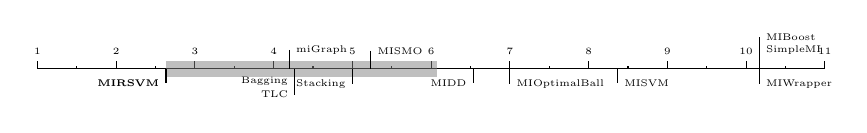
\begin{tikzpicture}
\draw (1,0) -- (11,0);
\foreach \x in {1,2,3,4,5,6,7,8,9,10,11} {
\draw (\x, 0) -- ++(0,.1) node [above,scale=0.7] {\tiny \x};
\ifthenelse{\x < 11}{\draw (\x+.5, 0) -- ++(0,.03);}{}
}

\coordinate (c0) at (2.6333,0);
\coordinate (c1) at (4.2,0);
\coordinate (c2) at (10.1667,0);
\coordinate (c3) at (7,0);
\coordinate (c4) at (6.5333,0);
\coordinate (c5) at (10.1667,0);
\coordinate (c6) at (5.2333,0);
\coordinate (c7) at (8.3667,0);
\coordinate (c8) at (10.1667,0);
\coordinate (c9) at (4.2667,0);
\coordinate (c10) at (4.2667,0);
\coordinate (c11) at (5,0);

\node (l0) at (c0) [below left=.05cm and 0cm, align=right,scale=0.7] {\tiny \textbf{MIRSVM}};
\node (l1) at (c1) [above right=.1cm and 0cm, align=left,scale=0.7] {\tiny miGraph};
\node (l2) at (c2) [above right=.27cm and 0cm, align=right,scale=0.7] {\tiny MIBoost};
\node (l3) at (c3) [below right=.05cm and 0cm, align=left,scale=0.7] {\tiny MIOptimalBall};
\node (l4) at (c4) [below left=.05cm and 0cm, align=right,scale=0.7] {\tiny MIDD};
\node (l5) at (c5) [below right=.05cm and 0cm, align=left,scale=0.7] {\tiny MIWrapper};
\node (l6) at (c6) [above right=.1cm and 0cm, align=left,scale=0.7] {\tiny MISMO};
\node (l7) at (c7) [below right=.05cm and 0cm, align=left,scale=0.7] {\tiny MISVM};
\node (l8) at (c8) [above right=.1cm and 0cm, align=left,scale=0.7] {\tiny SimpleMI};
\node (l9) at (c9) [below left=.2cm and 0cm, align=right,scale=0.7] {\tiny TLC};
\node (l10) at (c10) [below left=.02cm and 0cm, align=right,scale=0.7] {\tiny Bagging};
\node (l11) at (c11) [below left=.05cm and 0cm, align=right,scale=0.7] {\tiny Stacking};

\fill[fill=gray,fill opacity=0.5] (2.6333,-0.1) rectangle (6.0683,0.1);

\foreach \x in {0,1,2,3,4,5,6,7,8,9,10,11} {
\draw (l\x) -| (c\x);
};
\end{tikzpicture}}\vspace{-1.8em}
\captionof{figure}{Bonferroni-Dunn test for Cohen's Kappa rate}\label{fig:BonfDunnkappa}
\vspace{-1.3em}
\captionof{table}{Holm and Wilcoxon tests for Cohen's Kappa rate}\label{tab:statkappa}
\scriptsize
\resizebox{0.95\textwidth}{!}{\begin{tabular}{lccccccccccc}
\noalign{\smallskip}\hline\noalign{\smallskip}
MIRSVM vs. &miGraph &MIBoost &MIOptimalBall &MIDD &MIWrapper &MISMO &MISVM &SimpleMI &TLC &Bagging &Stacking \\
\noalign{\smallskip}\hline\noalign{\smallskip}
Holm $p$-value &0.0500 &0.0045 &0.0071 &0.0083 &0.0050 &0.0100 &0.0063 &0.0056 &0.0167 &0.0250 &0.0125 \\\noalign{\smallskip}\hline\noalign{\smallskip}
Wilcoxon $p$-value &0.0121 &0.0001 &0.0012 &0.0012 &0.0001 &0.0006 &0.0001 &0.0001 &0.1205 & 0.2077 &0.0946 \\
Wilcoxon R$^+$ &91.500 &120.00 &113.00 &113.00 &120.00 &115.00 &119.00 &120.00 &88.000 &83.000 &90.000 \\
Wilcoxon R$^-$ &13.500 &0.0000 &7.0000 &7.0000 &0.0000 &5.0000 &1.0000 &0.0000 &32.000 &37.000 &30.000 \\
\noalign{\smallskip}\hline\noalign{\smallskip}
\end{tabular}}
\end{table}
Table~\ref{tab:kappaResults} shows the Cohen's Kappa rate results obtained by the algorithms. These results support the accuracy achieved by the algorithms, in the sense that the instance-based and wrapper methods perform worse than bag-based and ensemble learners. MIRSVM's kappa values all fall within the range ($0.5$-$1$], indicating that its merit as a classifier agrees with the class distribution and is not random. Note that MIOptimalBall, MIDD, MISVM, MISMO, and Stacking contain some negative kappa values, indicating performance worse than the default-hypothesis. MIBoost, SimpleMI, and MIWrapper are shown to randomly classify all $15$ datasets. Figure~\ref{fig:BonfDunnkappa} and Table~\ref{tab:statkappa} show the results of the statistical analysis on the Cohen's Kappa Rate results. The Holm and Wilcoxon procedures reflect results similar to the Bonferroni-Dunn test, where MIRSVM performs significantly better than MIOptimalBall, MIDD, MISVM, MIWrapper, MIBoost, and SimpleMI, having $p$-values $< 0.01$. This supports MIRSVM's performance as a competitive classifier.

\subsection{Area Under ROC Curve}
\begin{table}[b!]
\caption{AUC for MI classifiers}\label{tab:aucResults}
\resizebox{0.95\textwidth}{!}{\begin{tabular}{lccccccccccccc}
\hline\noalign{\smallskip}
Datasets &MIRSVM & miGraph & MIBoost &MIOptimalBall &MIDD &MIWrapper &MISMO &MISVM &SimpleMI &TLC &Bagging &Stacking \\
\hline\noalign{\smallskip}
suramin &\textbf{0.8333} &\textbf{0.8333} &0.5000 &0.7250 &0.4250 &0.5000 &0.7250 &0.5000 &0.5000 &0.6000 &0.6650 &0.4524 &  \\
eastWest &\textbf{0.8000} &0.7000 &0.5000 &0.7250 &0.6125 &0.5000 &0.7125 &0.5625 &0.5000 &0.6000 &0.6000 &0.4500 &  \\
westEast &0.7500 &0.7500 &0.5000 &0.3750 &0.4500 &0.5000 &0.7375 &0.4125 &0.5000 &0.5625 &\textbf{0.8456} &0.6375 &  \\
musk1 &\textbf{0.9005} &0.8135 &0.5000 &0.7676 &0.8797 &0.5000 &0.7816 &0.7589 &0.5000 &0.8589 &0.6837 &0.8589 &  \\
musk2 &\textbf{0.8406} &0.6904 &0.5000 &0.7432 &0.6981 &0.5000 &0.6772 &0.6900 &0.5000 &0.6317 &0.6732 &0.6435 &  \\
webmining &0.6320 &0.5000 &0.5000 &0.5096 &0.5000 &0.5000 &0.7184 &0.8098 &0.5000 &0.6837 &\textbf{0.8123} &0.6048 &  \\
trx &0.6500 &0.6170 &0.5000 &\textbf{0.7392} &0.6932 &0.5000 &0.5000 &0.5000 &0.5000 &0.6732 &0.6450 &0.6281 &  \\
mutagenesis-atoms &0.7106 &0.7137 &0.5000 &0.5824 &0.6186 &0.5000 &0.6420 &0.5000 &0.5000 &\textbf{0.7257} &\textbf{0.7257} &0.7137 &  \\
mutagenesis-bonds &0.7856 &0.7455 &0.5000 &0.6578 &0.6981 &0.5000 &0.7850 &0.5000 &0.5000 &0.8012 &0.8012 &\textbf{0.8211} &  \\
mutagenesis-chains &\textbf{0.8252} &0.7417 &0.5000 &0.6142 &0.7257 &0.5000 &0.8051 &0.5000 &0.5000 &0.8170 &0.8170 &0.8130 &  \\
tiger &0.7750 &0.7950 &0.5000 &0.5000 &0.7100 &0.5000 &0.7200 &0.7550 &0.5000 &0.6650 &\textbf{0.8000} &0.7250 &  \\
elephant &0.8200 &\textbf{0.8300} &0.5000 &0.5000 &0.7900 &0.5000 &0.8100 &0.8000 &0.5000 &0.8000 &0.5625 &0.8250 &  \\
fox &0.6550 &0.6300 &0.5000 &0.5000 &0.5800 &0.5000 &0.5250 &0.4750 &0.5000 &0.6450 &\textbf{0.8589} &0.6500 &  \\
component &0.7855 &0.7496 &0.5000 &0.5536 &0.6033 &0.5000 &0.6272 &0.5201 &0.5000 &\textbf{0.8123} &0.6000 &0.8081 &  \\
function &0.7563 &0.7698 &0.5000 &0.5298 &0.6015 &0.5000 &0.6391 &0.5268 &0.5000 &\textbf{0.8456} &0.6317 &0.8434 &  \\
\noalign{\smallskip}\hline\noalign{\smallskip}
Average &\textbf{0.7680} &0.7253 &0.5000 &0.6015 &0.6390 &0.5000 &0.6937 &0.5874 &0.5000 &0.7148 &0.7148 &0.6983 &  \\
Rank &\textbf{2.7667} &4.2667 &10.1667 &7.0000 &6.5333 &10.1667 &5.2333 &8.2333 &10.1667 &4.2667 &4.2667 &4.9333 &  \\
\hline\noalign{\smallskip}
\end{tabular}}
\centering
\resizebox{0.95\textwidth}{!}{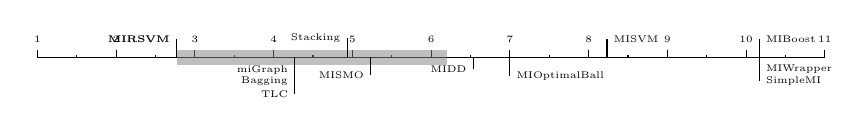
\begin{tikzpicture}
\draw (1,0) -- (11,0);
\foreach \x in {1,2,3,4,5,6,7,8,9,10,11} {
\draw (\x, 0) -- ++(0,.1) node [above,scale=0.7] {\tiny \x};
\ifthenelse{\x < 11}{\draw (\x+.5, 0) -- ++(0,.03);}{}
}

\coordinate (c0) at (2.7667,0);
\coordinate (c1) at (4.2667,0);
\coordinate (c2) at (10.1667,0);
\coordinate (c3) at (7,0);
\coordinate (c4) at (6.5333,0);
\coordinate (c5) at (10.1667,0);
\coordinate (c6) at (5.2333,0);
\coordinate (c7) at (8.2333,0);
\coordinate (c8) at (10.1667,0);
\coordinate (c9) at (4.2667,0);
\coordinate (c10) at (4.2667,0);
\coordinate (c11) at (4.9333,0);

\node (l0) at (c0) [above left=.1cm and 0cm, align=right,scale=0.7] {\tiny \textbf{MIRSVM}};
\node (l1) at (c1) [below left=.02cm and 0cm, align=right,scale=0.7] {\tiny miGraph};
\node (l2) at (c2) [above right=.1cm and 0cm, align=left,scale=0.7] {\tiny MIBoost};
\node (l3) at (c3) [below right=.1cm and 0cm, align=left,scale=0.7] {\tiny MIOptimalBall};
\node (l4) at (c4) [below left=.02cm and 0cm, align=right,scale=0.7] {\tiny MIDD};
\node (l5) at (c5) [below right=.01cm and 0cm, align=left,scale=0.7] {\tiny MIWrapper};
\node (l6) at (c6) [below left=.1cm and 0cm, align=right,scale=0.7] {\tiny MISMO};
\node (l7) at (c7) [above right=.1cm and 0cm, align=left,scale=0.7] {\tiny MISVM};
\node (l8) at (c8) [below right=.16cm and 0cm, align=left,scale=0.7] {\tiny SimpleMI};
\node (l9) at (c9) [below left=.34cm and 0cm, align=right,scale=0.7] {\tiny TLC};
\node (l10) at (c10) [below left=.16cm and 0cm, align=right,scale=0.7] {\tiny Bagging};
\node (l11) at (c11) [above left=.1cm and 0cm, align=right,scale=0.7] {\tiny Stacking};

\fill[fill=gray,fill opacity=0.5] (2.7667,-0.1) rectangle (6.2017,0.1);

\foreach \x in {0,1,2,3,4,5,6,7,8,9,10,11} {
\draw (l\x) -| (c\x);
};
\end{tikzpicture}}\vspace{-1.8em}
\captionof{figure}{Bonferroni-Dunn test for AUC}\label{fig:BonfDunnauc}\vspace{-1.3em}
\captionof{table}{Holm and Wilcoxon tests for AUC}\label{tab:statauc}
\scriptsize
\resizebox{0.95\textwidth}{!}{\begin{tabular}{lccccccccccc}
\noalign{\smallskip}\hline\noalign{\smallskip}
MIRSVM vs. &miGraph &MIBoost &MIOptimalBall &MIDD &MIWrapper &MISMO &MISVM &SimpleMI &TLC &Bagging &Stacking \\
\noalign{\smallskip}\hline\noalign{\smallskip}
Holm $p$-value &0.0167 &0.0045 &0.0071 &0.0083 &0.0050 &0.0100 &0.0063 &0.0056 &0.0250 &0.0500 &0.0125 \\\noalign{\smallskip}\hline\noalign{\smallskip}
Wilcoxon $p$-value &0.0166 &0.0001 &0.0002 &0.0003 &0.0001 &0.0012 &0.0009 &0.0001 & 0.2523 & 0.3028 &0.0781 \\
Wilcoxon R$^+$ &90.000 &120.00 &118.00 &117.00 &120.00 &113.00 &114.00 &120.00 &81.000 &79.000 &91.500 \\
Wilcoxon R$^-$ &15.000 &0.0000 &2.0000 &3.0000 &0.0000 &7.0000 &6.0000 &0.0000 &39.000 &41.000 &28.500 \\
\noalign{\smallskip}\hline\noalign{\smallskip}
\end{tabular}}
\end{table}
Table~\ref{tab:aucResults} shows AUC results obtained by the algorithms, which complement the accuracy and kappa rate, emphasizing the better performance of bag-based methods. MIRSVM achieves the best AUC score on $5$ of the $15$ datasets, while MIBoost, SimpleMI, and MIWrapper obtain the worst results. Their AUC score indicates random predictor behavior, having values $= 0.5$. Bag-level methods all obtain scores between $0.7$ and $0.77$ indicating a high true positive rate and a low false positive rate, which is reflected by the precision and recall results. Figure~\ref{fig:BonfDunnauc} and Table~\ref{tab:statauc} show that MIRSVM performs significantly better than $6$ out of the $11$ competing algorithms. Holm's procedure indicates that significant differences exist between MIRSVM and all algorithms except miGraph, TLC, Bagging, and Stacking. MISVM's true positive rate could be affected because of the possible imbalance of support vectors from the positive and negative classes (favoring the negative). Note that the Wilcoxon $p$-values for MIWrapper, MIBoost, and SimpleMI are $0.0001$. 

\subsection{Overall Comparison}
\begin{table}[t!]
\centering
\caption{Run Time (seconds) for MI classifiers}\label{tab:time}
\resizebox{0.95\textwidth}{!}{\begin{tabular}{lrrrrrrrrrrrrr}
\hline\noalign{\smallskip}
Datasets &MIRSVM & miGraph & MIBoost &MIOptimalBall &MIDD &MIWrapper &MISMO &MISVM &SimpleMI &TLC &Bagging &Stacking \\
\hline\noalign{\smallskip}
suramin &\textbf{0.1} &19.7 &8.8 &30.5 &7922.0 &9.5 &52.3 &333.9 &7.2 &35.5 &183.0 &90.6 &  \\
eastWest &\textbf{0.1} &3.0 &5.5 &9.4 &217.1 &6.3 &14.8 &21.4 &5.8 &15.4 &15.4 &15.2 &  \\
westEast &\textbf{0.1} &2.8 &6.5 &7.8 &79.7 &6.5 &14.7 &99.5 &6.0 &16.6 &12128.1 &10.8 &  \\
musk1 &\textbf{0.4} &56.8 &13.4 &32.1 &3542.6 &20.6 &89.7 &198.4 &11.1 &93.0 &86272.6 &759.5 &  \\
musk2 &\textbf{2.3} &452.3 &97.3 &782.9 &126016.8 &208.3 &1799.4 &26093.5 &16.1 &1772.2 &2229.3 &16759.0 &  \\
webmining &\textbf{300.6} &302.5 &45745.4 &60474.8 &47601.4 &68736.7 &51923.6 &105622.3 &2685.9 &86272.6 &9861.5 &592948.9 &  \\
trx &61.8 &2206.4 &17.6 &682.3 &339110.5 &19.3 &8670.3 &134622.1 &\textbf{7.4} &2229.3 &243.3 &11927.9 &  \\
mutagenesis-atoms &9.8 &193.1 &8.8 &99.2 &2623.0 &8.0 &55.0 &53.5 &\textbf{6.4} &44.0 &44.0 &153.9 &  \\
mutagenesis-bonds &\textbf{8.3} &410.3 &10.2 &310.2 &17538.7 &12.3 &457.4 &2794.8 &8.4 &131.1 &131.1 &853.1 &  \\
mutagenesis-chains &19.3 &513.4 &12.0 &525.0 &48982.7 &14.8 &2451.9 &6637.4 &\textbf{7.2} &224.4 &224.4 &1619.0 &  \\
tiger &29.5 &302.8 &44.5 &157.8 &23220.5 &56.2 &208.0 &608.8 &\textbf{16.2} &183.0 &212.1 &1085.0 &  \\
elephant &47.7 &306.7 &45.5 &243.9 &56456.2 &69.7 &232.1 &1114.3 &20.8 &212.1 &\textbf{16.6} &1462.2 &  \\
fox &81.0 &303.1 &44.2 &206.1 &27773.8 &66.0 &369.6 &891.5 &\textbf{23.5} &243.3 &93.0 &1729.1 &  \\
component &231.7 &3091.0 &572.5 &228209.6 &96263.9 &1096.9 &629366.4 &37224.6 &144.0 &9861.5 &\textbf{35.5} &79149.8 &  \\
function &740.3 &8162.7 &935.5 &768458.0 &350124.7 &1887.5 &1052225.3 &565026.4 &\textbf{232.8} &12128.1 &1772.2 &185918.5 &  \\
\noalign{\smallskip}\hline\noalign{\smallskip}
Average &\textbf{102.2} &1088.4 &3171.2 &70682.0 &76498.2 &4814.6 &116528.7 &58756.2 &213.3 &7564.1 &7564.1 &59632.2 &  \\
Rank &2.3 &6.2 &3.1 &7.2 &11.1 &4.3 &8.5 &10.1 &\textbf{1.9} &7.2 &6.5 &9.7 &  \\
\hline\noalign{\smallskip}
\end{tabular}}
\captionof{table}{Overall ranks comparison for MI classifiers}\label{tab:metarank}
\resizebox{0.95\textwidth}{!}{\begin{tabular}{lccccccccccccc}
\hline\noalign{\smallskip}
Ranks &MIRSVM & miGraph & MIBoost &MIOptimalBall &MIDD &MIWrapper &MISMO &MISVM &SimpleMI &TLC &Bagging &Stacking \\
\midrule
Accuracy &\textbf{2.2000} &3.8667 &9.6000 &7.8667 &6.5667 &9.6000 &5.3333 &8.5667 &9.6000 &4.7000 &4.8667 &5.2333 &  \\
Precision &\textbf{5.3333} &6.1333 &7.1000 &7.3333 &7.3667 &7.1000 &5.8667 &5.8667 &7.1000 &5.9000 &6.3333 &6.5667 &  \\
Recall &4.8667 &6.5667 &6.8667 &6.3333 &7.3667 &6.8667 &6.7000 &7.4333 &\textbf{4.8333} &7.3667 &6.0667 &6.7333 &  \\
Kappa &\textbf{2.6333} &4.2000 &10.1667 &7.0000 &6.5333 &10.1667 &5.2333 &8.3667 &10.1667 &4.2667 &4.2667 &5.0000 &  \\
AUC &\textbf{2.7667} &4.2667 &10.1667 &7.0000 &6.5333 &10.1667 &5.2333 &8.2333 &10.1667 &4.2667 &4.2667 &4.9333 &  \\
Time &2.2667 &6.2000 &3.1000 &7.2000 &11.0667 &4.3000 &8.5333 &10.1333 &\textbf{1.8667} &7.2000 &6.4667 &9.6667 &  \\
\noalign{\smallskip}\hline\noalign{\smallskip}
Average &\textbf{3.3444} &5.2056 &7.8333 &7.1222 &7.5722 &8.0333 &6.1500 &8.1000 &7.2889 &5.6167 &5.3778 &6.3556 &  \\
Rank &\textbf{1.3333} &3.6667 &8.9167 &7.7500 &9.2500 &9.0833 &5.9167 &8.7500 &7.3333 &5.2500 &4.2500 &6.5000 &  \\
\hline\noalign{\smallskip}
\end{tabular}}
\centering
\resizebox{0.95\textwidth}{!}{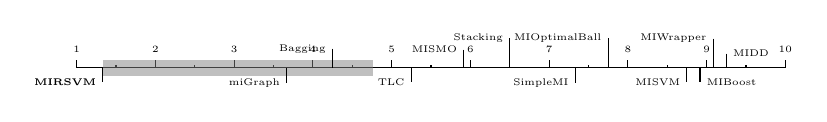
\begin{tikzpicture}
\draw (1,0) -- (10,0);
\foreach \x in {1,2,3,4,5,6,7,8,9,10} {
\draw (\x, 0) -- ++(0,.1) node [above,scale=0.7] {\tiny \x};
\ifthenelse{\x < 10}{\draw (\x+.5, 0) -- ++(0,.03);}{}
}

\coordinate (c0) at (1.3333,0);
\coordinate (c1) at (3.6667,0);
\coordinate (c2) at (8.9167,0);
\coordinate (c3) at (7.75,0);
\coordinate (c4) at (9.25,0);
\coordinate (c5) at (9.0833,0);
\coordinate (c6) at (5.9167,0);
\coordinate (c7) at (8.75,0);
\coordinate (c8) at (7.3333,0);
\coordinate (c9) at (5.25,0);
\coordinate (c10) at (4.25,0);
\coordinate (c11) at (6.5,0);

\node (l0) at (c0) [below left=.05cm and 0cm, align=right,scale=0.7] {\tiny \textbf{MIRSVM}};
\node (l1) at (c1) [below left=.05cm and 0cm, align=right,scale=0.7] {\tiny miGraph};
\node (l2) at (c2) [below right=.05cm and 0cm, align=left,scale=0.7] {\tiny MIBoost};
\node (l3) at (c3) [above left=.23cm and 0cm, align=right,scale=0.7] {\tiny MIOptimalBall};
\node (l4) at (c4) [above right=.05cmand 0cm, align=left,scale=0.7] {\tiny MIDD};
\node (l5) at (c5) [above left=.23cm and 0cm, align=right,scale=0.7] {\tiny MIWrapper};
\node (l6) at (c6) [above left=.1cm and 0cm, align=right,scale=0.7] {\tiny MISMO};
\node (l7) at (c7) [below left=.05cm and 0cm, align=right,scale=0.7] {\tiny MISVM};
\node (l8) at (c8) [below left=.05cm and 0cm, align=right,scale=0.7] {\tiny SimpleMI};
\node (l9) at (c9) [below left=.05cm and 0cm, align=right,scale=0.7] {\tiny TLC};
\node (l10) at (c10) [above left=.1cm and 0cm, align=right,scale=0.7] {\tiny Bagging};
\node (l11) at (c11) [above left=.23cm and 0cm, align=right,scale=0.7] {\tiny Stacking};

\fill[fill=gray,fill opacity=0.5] (1.3333,-0.1) rectangle (4.7683,0.1);

\foreach \x in {0,1,2,3,4,5,6,7,8,9,10,11} {
\draw (l\x) -| (c\x);
};
\end{tikzpicture}}\vspace{-1.8em}
\captionof{figure}{Bonferroni-Dunn test for overall ranks comparison}\label{fig:BonfDunnpmeta}
\end{table}
Table~\ref{tab:time} shows the run times, in seconds, for each algorithm. MIRSVM has the fastest run time and is ranked second. MIRSVM shows very good scalability considering the number of features, such as in the webmining dataset which comprises of $5863$ attributes. Additionally, taking into account the number of instances as seen in the two largest datasets, component and function, MIRSVM displays superior scalability. It is important to note that quadratic programming solvers are not the most efficient tools for solving optimization problems in terms of run time, and yet MIRSVM still is shown to perform competitively against the current widely used algorithms. The scalability of MIRSVM is founded on the speedy rate of bag-representative convergence, as shown previously in Figure~\ref{fig:convegence}.

SimpleMI achieves the highest rank and competitive run times because, rather than use the instances in each bag to train a model, it takes the mean value of the instances in a bag and uses that for training. Even though SimpleMI has fast run-times, its performance over the previous metrics has been shown to be random and not as effective as the bag-level methods.

Table~\ref{tab:metarank} shows the ranks achieved by each of the metrics along with the average and meta-ranks, to illustrate the overall performance across all metrics. MIRSVM has the best meta-rank (rank of the ranks) and the miGraph method has the second best. The meta-ranks also highlight the better performance of bag-level methods over instance-level and wrapper methods, emphasizing the importance of training at the bag-level. Not only does MIRSVM use bag-level information during classification, but it also optimizes over the instances within the bag, which helps determine which instances contribute the most information about the bags label. SimpleMI, MIWrapper, MIBoost, MISVM, and MDD have the worst performance compared to MIRSVM and miGraph. Specifically, it is evident from the precision and recall results that MIBoost, MIWrapper, and SimpleMI, for example, classify all bags as negative for datasets that have imbalanced class distributions which favor the negative class. This emphasizes the disadvantage of using wrapper methods and assuming the data distribution of the instances within positive bags. Although these algorithms are popular in literature, the experimental study clearly shows that recent bag-level and ensemble methods easily overcome traditional multi-instance learning algorithms. 

In summary, MIRSVM offers improvement in terms of both accuracy and run-time when compared to referenced methods, especially those utilizing SVM-based algorithms.

\section{Conclusions}
This proposal consisted of a novel formulation and algorithm for the multiple-instance support vector machine problem, which optimizes bag classification via bag-representative selection. First, the primal formulation was posed and its dual was then derived and solution computed using a quadratic programming solver. This formulation was designed to utilize bag-level information and find an optimal separating hyperplane between bags, rather than individual instances, using the standard multi-instance assumption. The SMI assumption states that a bag is labeled positive if and only if at least one instance within a bag is positive, and is negative otherwise. The key features of the proposed algorithm MIRSVM are its ability to identify instances within positive and negative bags, i.e. the support vectors or representatives, that highly impact the decision boundary and margin, as well as avoiding uncertainties and issues caused by techniques that flatten, subset, or under-represent positive instances within positively labeled bags. Additionally, it exhibits desirable convergence and scalability, making it suitable for large-scale learning tasks.

The experimental study showed the better performance of MIRSVM compared with existing multi-instance support vector machines, traditional multi-instance learners, as well as ensemble methods. The results, according to a variety of performance metrics, were compared and further validated using statistical analysis with non-parametric tests which highlight the advantages of using bag-level based and ensemble learners, such as miGraph, Bagging, and Stacking, while showing the instance-level based learners performed poorly in comparison or were deemed as strongly biased and unstable classifiers. Our proposal, MIRSVM, performs statistically better, neither compromising accuracy nor run-time while displaying a robust performance across all of the evaluated datasets. The research outcomes of this chapter have been published in~\cite{melki2018mirsvm}.

\chapter{Conclusions}
This thesis introduced four novel SVM algorithms for learning from the non-standard and diverse learning paradigms: multi-target regression and multi-instance classification. 

Three unique approaches for multi-target regression were proposed: the baseline problem transformation support vector regressor SVR, an ensemble of randomly generated chains using this base model SVRRC, and a maximally correlated chained model SVRCC. The results highlighted the better performance of SVR as a base model, however, because it is a problem transformation method, the possible correlations amongst the targets are lost on the final model. SVRRC was designed to test whether taking these correlations into account would benefit the final learning model, and the results showed a performance increase. However, due to the random nature of SVRRC, capturing target correlations is not guaranteed. SVRCC was designed to remedy this issue using a maximum correlation chain and proved to capture target correlations accurately, providing the best results among the contributions, as well as against the methods compared. 

A novel multiple-instance bag-level formulation and algorithm, dubbed MIRSVM, with a bag-representative selector, are proposed. The algorithm trains the SVM on bag-level information, iteratively selecting the best representative instance for each positive and negative bag, while finding the optimal separating hyperplane. This approach, unlike other existing ones, eliminates possible class imbalance issues by allowing both positive and negative bags to be represented. The experimental and statistical study showed that bag-level learners outperform instance-level learners and wrapper methods. MIRSVM outperformed current contemporary SVM multi-instance algorithms, as well as other algorithms of different classes. 


\chapter{Future Work}
The contributions introduced in this work highlight the performance quality of SVMs for solving difficult learning problems. The SVM solvers used were LIBSVM's SMO implementation and MATLAB's standard QP solver. Even though the proposals outperformed existing popular algorithms in each learning paradigm, these two popular and standard solvers have some disadvantages. Although SMO provides an exact solution to the SVM QP problem, its performance is highly dependent on the SVM hyperparameters and MATLAB's QP solver is notoriously dependent on the size and complexity of the data. To address these problems, the future work of this dissertation first aims to deal with these limitations without sacrificing accuracy for scalability with respect to large-scale problems, while maintaining applicability to small and medium sized datasets. 

Stochastic gradient descent (SGD) methods are popular tools used to optimize large-scale learning problems because of their generalization performance, simplicity, and scalability. Recently, SGD algorithms have been shown to have considerable performance and generalization capabilities in the context of large-scale learning~\cite{bottou2010large}, and have been used to solve the SVM problem, such as \textit{NORMA}~\cite{kivinen2004online} and \textit{PEGASOS}~\cite{shalev2011pegasos,zhang2004solving}. Although stochastic and iterative algorithms are very simple to implement and efficient, they also have their limitations. One of these limitations is the lack of meaningful stopping criteria for the algorithm; without a pre-specified number of iterations to train, the algorithms continue running~\cite{panagiotakopoulos2013stochastic}. Another limitation stems from the superlinear increase in training time as the number of samples increases. Incremental algorithms attempt to alleviate this issue, but they cannot guarantee a bound on the number of updates per iteration~\cite{cauwenberghs2001incremental}. 

To address the limitations presented by current popular SVM solvers, the future work of this dissertation involves the following:
\begin{enumerate}
\iitem Devising a unique iterative procedure for solving the L1-SVM problem, as well as a novel method for identifying support vectors. Rather than randomly iterating over the data samples, the proposal will aim to reduce training time by selecting and updating the samples that are most incorrectly classified with respect to the current decision hyperplane.

\iitem Designing a novel stopping criteria by utilizing this support vector identification method. This aims to eliminate the added parameterization that is included with most online methods, where the number of iterations of the algorithm needs to be set in advance. Once there are no incorrectly classified samples left, the algorithm terminates.

\iitem Applying, experimenting, and analyzing the performance of the newly proposed method to a popular new online paradigm, learning from streaming data, where data is not persistent, rather it is transient over time. This challenging setting will test the new contribution's performance on not only a dynamic data representation, but also on how efficiently computational resources are being used when learning is constrained over time.
\end{enumerate}

\printbibliography[title={References}, heading=bibintoc]

\begin{comment}

\begin{appendices}
\titleformat{\chapter}[display]{\bfseries\centering}{\huge Appendix \thechapter}{1em}{\Huge #1}
\chapter{Publications}
\newpage
% MIRSVM
\thispagestyle{plain}
\begin{center}
    \vspace*{0.5 cm}
     \textsc{\LARGE MIRSVM: Multi-Instance SVM using Bag Representatives}\\[0.5 cm]
     \textsc{\textit{Authors: }Gabriella Melki, Alberto Cano, Sebastian Ventura}\\[0.5 cm]		
     
     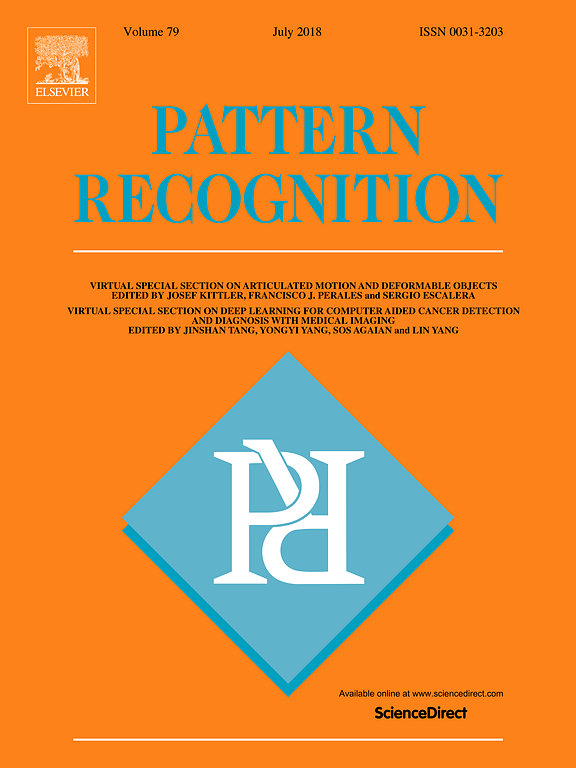
\includegraphics[scale = 0.25]{figures/pr.jpg}\\[0.5 cm]	
     \textsc{Pattern Recognition, Volume 79, pp. 228-241, July 2018}\\[0.5 cm]		
	
	\begin{minipage}{0.6\textwidth}
	\centering
		\textsc{Publisher: Elsevier}\\
	    	\textsc{Impact Factor: 4.582}\\
	    	\textsc{DOI:} 10.1016/j.patcog.2018.02.007 \\
	\end{minipage}\\[2 cm]
\end{center}
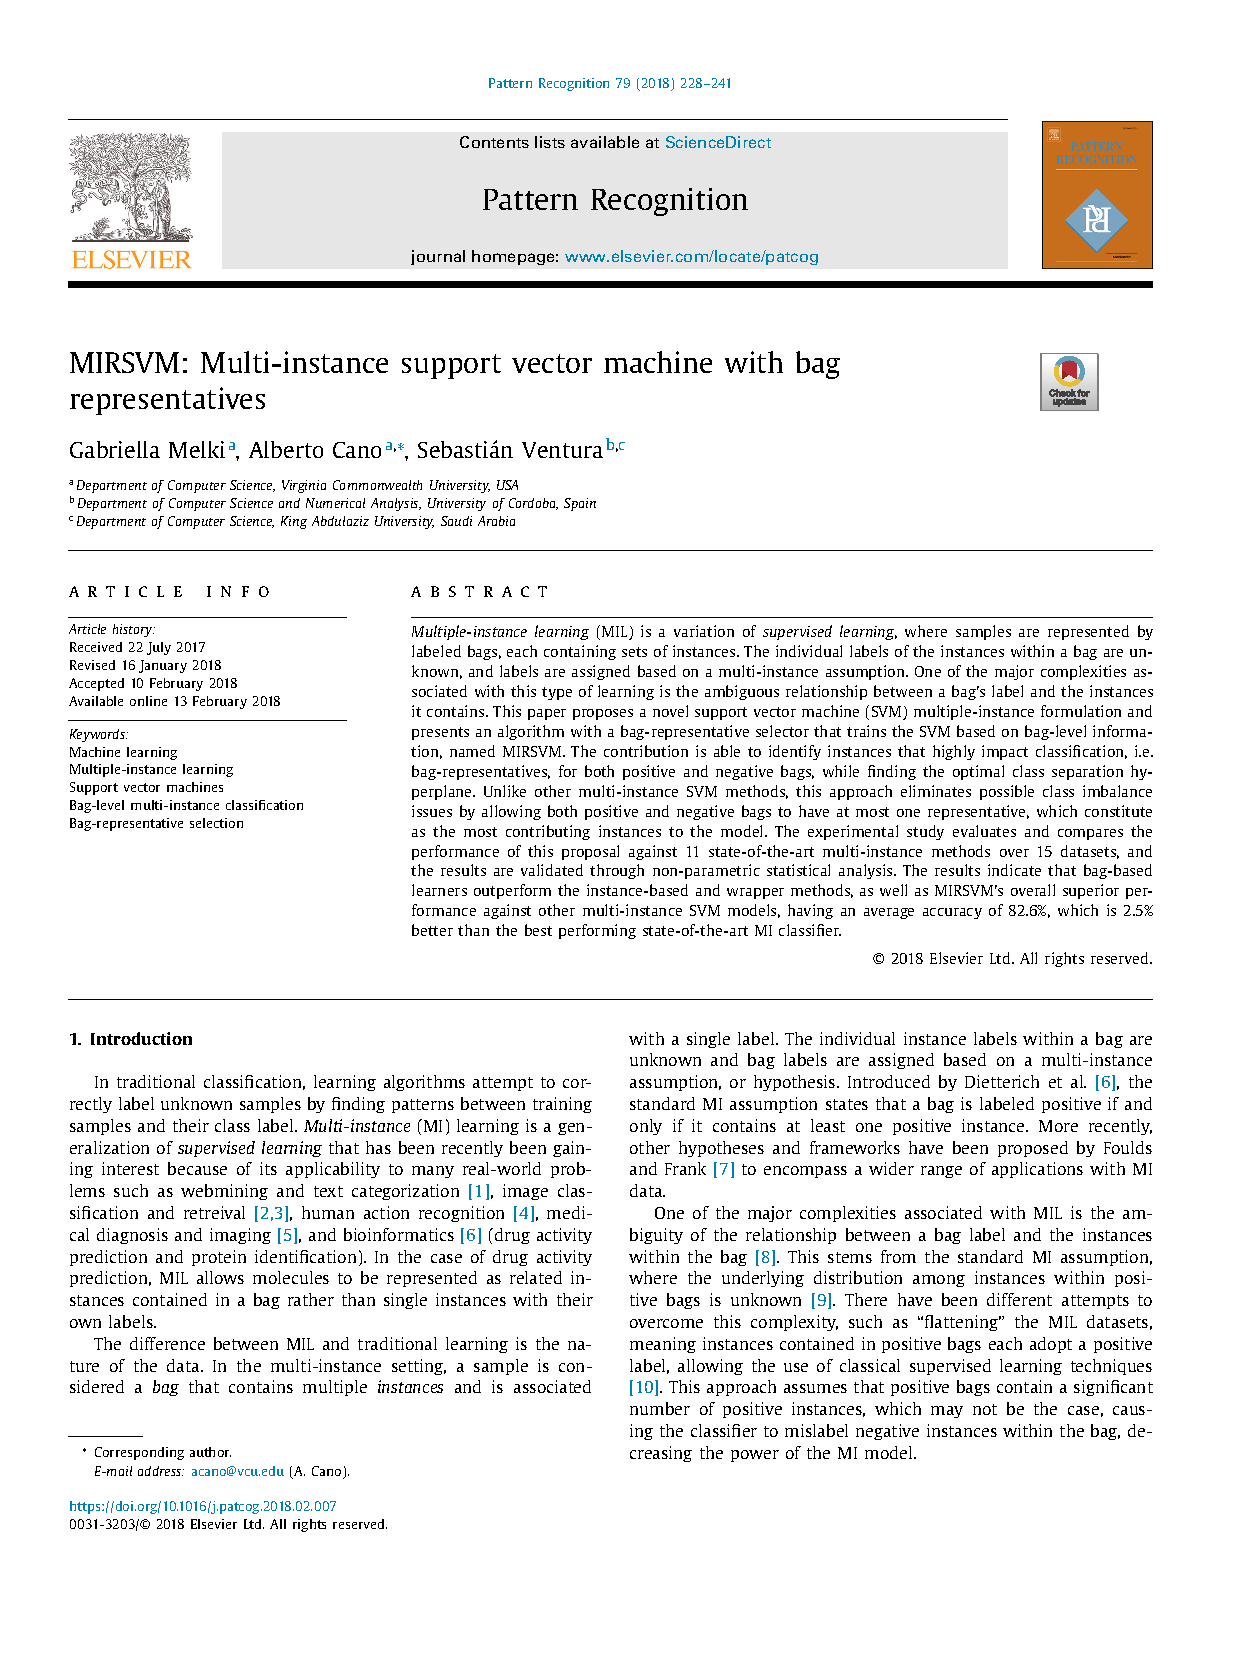
\includepdf[pages=1,pagecommand=\section{MIRSVM: Multi-Instance SVM with Bag Representatives},scale=.8,linktodoc=true]{publications/mirsvm.pdf}
\includepdf[pages={2-},scale=.8,linktodoc=true]{publications/mirsvm.pdf}


% MULTI_TARGET
\begin{center}
    \vspace*{0.5 cm}
     \textsc{\LARGE Multi-Target Support Vector Regression Via Correlation Regressor Chains}\\[0.5 cm]
     \textsc{\textit{Authors: }Gabriella Melki, Alberto Cano, Vojislav Kecman, Sebastian Ventura}\\[0.5 cm]		
     
     
\includegraphics[scale = 0.25]{figures/is.jpg}\\[0.5 cm]	
     \textsc{Information Sciences, Volumes 415–-416, pp. 53-69, November 2017}\\[0.5 cm]	
	
	\begin{minipage}{0.6\textwidth}
	\centering
		\textsc{Publisher: Elsevier}\\
	    	\textsc{Impact Factor: 4.832}\\
	    	\textsc{DOI:} 10.1016/j.ins.2017.06.017 \\
	\end{minipage}\\[2 cm]
\end{center}
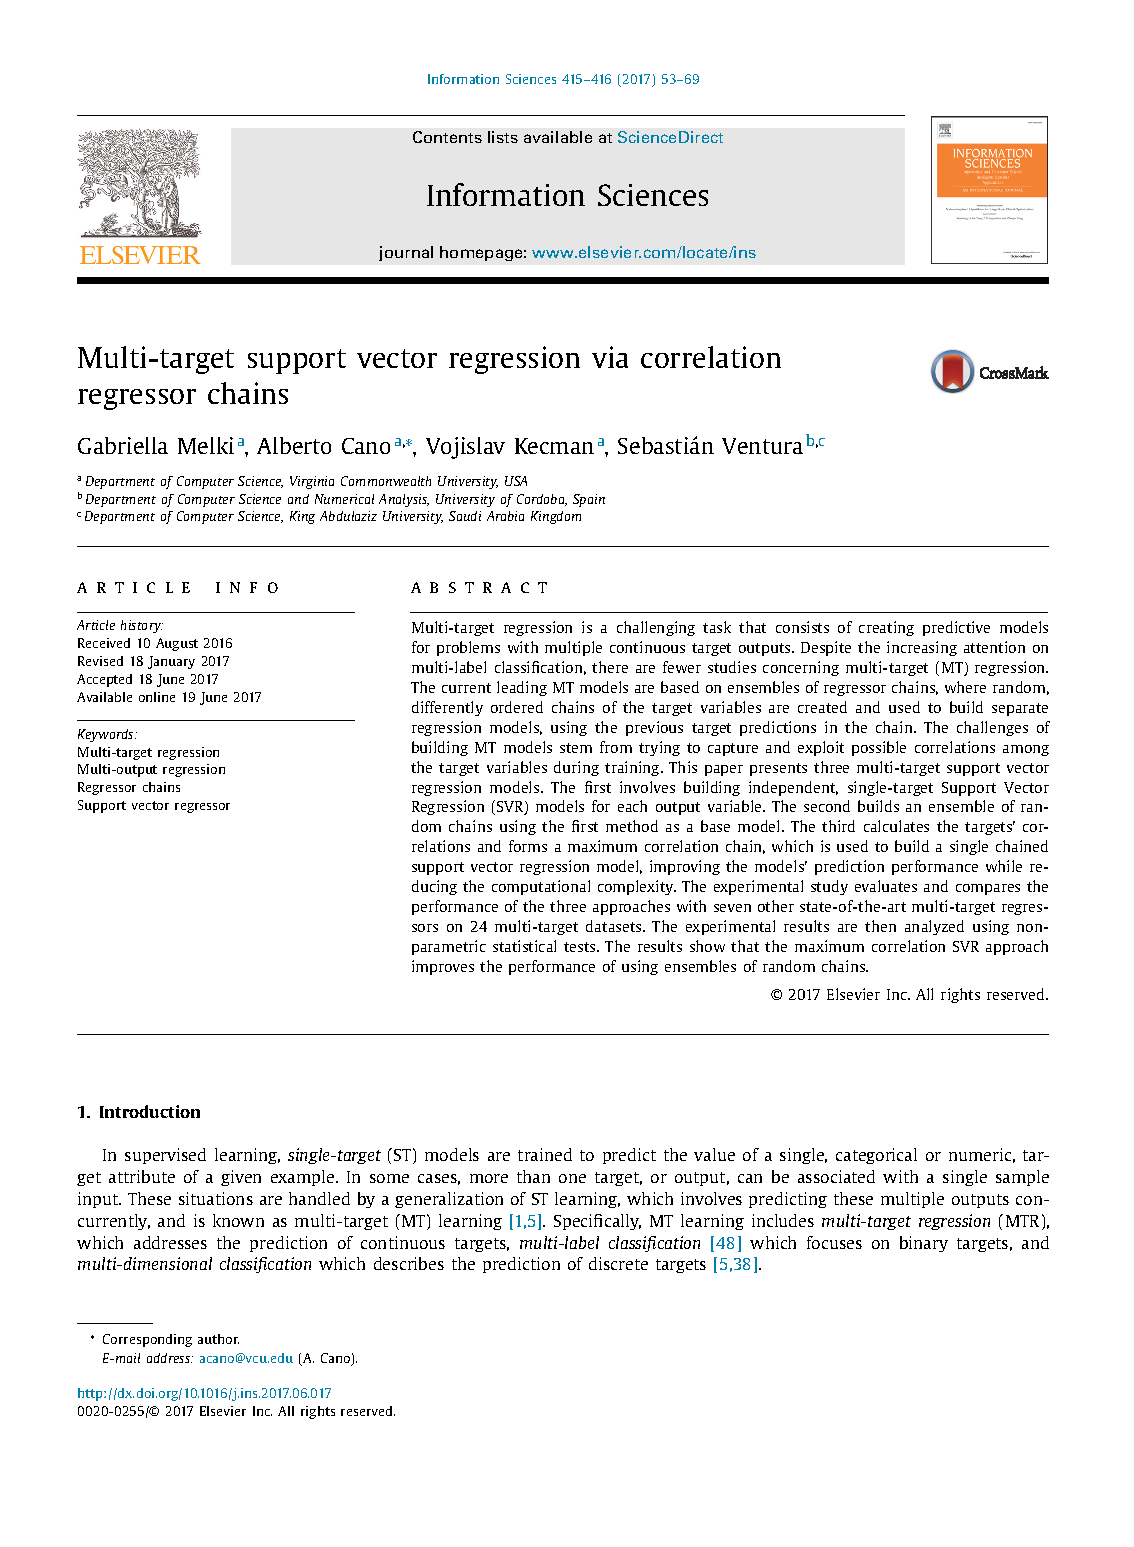
\includepdf[pages=1,pagecommand=\section{Multi-Target Support Vector Regression Via Correlation Regressor Chains},scale=.8,linktodoc=true]{publications/mtr.pdf}
\includepdf[pages={2-},scale=.8,linktodoc=true]{publications/mtr.pdf}

% ACRONYMS
\chapter{List of Acronyms}
\begin{longtable}{ p{.20\textwidth}  p{.80\textwidth} } 
\textbf{aCC} & Average Correlation Coefficient \\
\textbf{APR} & Axis Parallel Rectangle \\
\textbf{aRMSE} & Average Root Mean Squared Error \\
\textbf{aRRMSE} & Average Relative Root Mean Squared Error \\
\textbf{AUC} & Area Under ROC Curve \\
\textbf{BVM} & Ball Vector Machines \\
\textbf{CitationKNN} & Citation k-Nearest Neighbors \\
\textbf{CV} & Cross Validation \\
\textbf{CVM} & Core Vector Machines \\
\textbf{DD} & Diverse Density \\
\textbf{EM-DD} & Expectation-Maximization Diverse Density \\
\textbf{ERC} & Ensemble of Random Chains \\
\textbf{ERCC} & Ensemble of Random Chains Corrected \\
\textbf{FN} & False Negative \\
\textbf{FP} & False Positive \\
\textbf{ISDA} & Iterative Single Data Algorithm \\
\textbf{KNN} & k-Nearest Neighbors \\
\textbf{MI} & Multiple Instance \\
\textbf{miGraph} & Mixed Integer Graph \\
\textbf{MIL} & Multiple Instance Learning \\
\textbf{MIOptimalBall} & Multiple Instance Optimal Ball \\
\textbf{MIRI} & Multi-Instance Rule Induction \\
\textbf{MIRSVM} & Multi-Instance Support Vector Machine \\
\textbf{MISMO} & Multiple Instance Sequential Minimal Optimization \\
\textbf{MITI} & Multi-Instance Tree Inducer \\
\textbf{MNSVM} & Minimal Norm Support Vector Machine \\
\textbf{MORF} & Multi-Objective Random Forests \\
\textbf{MSE} & Mean Squared Error \\
\textbf{MT} & Multiple Target \\
\textbf{MTR} & Multiple Target Regression \\
\textbf{MTS} & Multiple Target Stacking \\
\textbf{MTSC} & Multiple Target Stacking Corrected \\
\textbf{NLSVR} & Non-Linear Support Vector Regressor \\
\textbf{NNISDA} & Non-Negative Iterative Single Data Algorithm \\
\textbf{NORMA} & "Na{\""}ve Online R Minimization Algorithm" \\
\textbf{OLLA} & Online Learning Algorithm \\
\textbf{PEGASOS} & Primal Estimated Sub-Gradient Solver for Support Vector Machines \\
\textbf{QP} & Quadratic Programming \\
\textbf{RC} & Random Chaining \\
\textbf{RCC} & Regression Chains Corrected \\
\textbf{ROC} & Receiver Operating Characteristic \\
\textbf{SGD} & Stochastic Gradient Descent \\
\textbf{SMI} & Standard Multiple Instance Assumption \\
\textbf{SMO} & Sequential Minimal Optimization \\
\textbf{SphereSVM} & Sphere Support Vector Machine \\
\textbf{SRM} & Structured Risk Minimization \\
\textbf{ST} & Single Target \\
\textbf{SVM} & Support Vector Machine \\
\textbf{SVR} & Support Vector Regressor \\
\textbf{SVRCC} & Support Vector Regressor with maximum Correlation Chaining \\
\textbf{SVRRC} & Support Vector Regressor with Random Chaining \\
\textbf{TLC} & Two-Level Classifier \\
\textbf{TN} & True Negative \\
\textbf{TP} & True Positive  \\
\end{longtable}

\end{appendices}

\end{comment}

\chapter*{Vita}
\thispagestyle{plain}
\addcontentsline{toc}{chapter}{Vita}
Gabriella Melki received her BSc. in Computer Science at the American University of Beirut in 2011 and her MSc. in Computer Science from Virginia Commonwealth University in 2016. As a full-time student in the dual Ph.D. program between Virginia Commonwealth University and the University of C\'{o}rdoba in Spain, her research is focused on machine learning algorithms for large datasets and different data representations. Her more specialized field of interest is support vector machines.

\textbf{Publications:}
\begin{itemize}
\item[-] \textbf{Melki G}, Kecman V, Ventura S, Cano A, ``OLLAWV: OnLine Learning using Worst-Violators", In: \textit{Applied Soft Computing} 66, (2018), pp. 384--393
\item[-] \textbf{Melki G}, Cano A, Ventura S, ``MIRSVM: Multi-Instance Support Vector Machine with Bag Representatives", In: \textit{Pattern Recognition} 75, (2018), pp. 228--214
\item[-] \textbf{Melki G}, Cano A, Kecman V, Ventura S, ``Multi-Target Support Vector Regression Via Correlation Regressor Chains", In: \textit{Information Sciences} 415, (2017), pp. 53--69
\item[-] \textbf{Melki G}, ``Fast Online Training of L1 Support Vector Machines", Master's Thesis, \textit{Virginia Commonwealth University}, (2016), pp. 1--64
\item[-] \textbf{Melki G}, Kecman V, ``Speeding Up Online Training of L1 Support Vector Machines", In: \textit{Proceedings of the IEEE SoutheastCon, 2016}, (2016), pp. 1--6
\item[-] Kecman V, \textbf{Melki G}, ``Fast Online Algorithm for SVMs", In: \textit{Proceedings of the IEEE SoutheastCon, 2016}. (2016), pp. 1--6
\end{itemize}

\end{document}
